\documentclass[11pt,oneside,reqno]{article}

\usepackage[T1]{fontenc}
\usepackage{amsmath,amssymb,amsthm}
\usepackage{mathpazo}
\usepackage[margin=1in]{geometry}
\usepackage{microtype}
\usepackage{array}
\usepackage{tikz-cd}
\usetikzlibrary{arrows.meta,calc,decorations.pathreplacing,positioning,patterns}
\usepackage[hidelinks]{hyperref}
\hypersetup{
  pdftitle={Expository notes on Brylinski--Getzler},
  pdfauthor={Expository notes on Brylinski--Getzler}
}

\DeclareMathOperator{\HH}{HH}
\DeclareMathOperator{\HC}{HC}
\DeclareMathOperator{\HP}{HP}
\DeclareMathOperator{\gr}{gr}
\DeclareMathOperator{\Tr}{Tr}
\DeclareMathOperator{\tr}{tr}
\DeclareMathOperator{\res}{res}
\DeclareMathOperator{\Res}{Res}
\DeclareMathOperator{\sgn}{sgn}
\DeclareMathOperator{\supp}{supp}
\DeclareMathOperator{\Op}{Op}
\DeclareMathOperator{\Tor}{Tor}
\DeclareMathOperator{\Ext}{Ext}
\DeclareMathOperator{\ad}{ad}
\DeclareMathOperator{\Ker}{ker}
\DeclareMathOperator{\Ran}{im}
\newcommand{\C}{\mathbb C}
\newcommand{\R}{\mathbb R}
\newcommand{\Z}{\mathbb Z}
\newcommand{\N}{\mathbb N}
\newcommand{\cA}{\mathcal A}
\newcommand{\cB}{\mathcal B}
\newcommand{\cD}{\mathcal D}
\newcommand{\cE}{\mathcal E}
\newcommand{\cP}{\mathcal P}
\newcommand{\cO}{\mathcal O}
\newcommand{\cL}{\mathcal L}
\newcommand{\CI}{C^\infty}
\newcommand{\Om}{\Omega}
\newcommand{\hot}{\mathbin{\widehat\otimes}}
\newcommand{\Tdot}{\dot T^*}
\newcommand{\Sst}{S^*\!M}
\newcommand{\eps}{\varepsilon}
\newcommand{\Lie}{\mathcal L}
\newcommand{\vol}{\mathrm{vol}}
\newcommand{\hb}{\hbar}
\newcommand{\Lser}[1]{(\!(#1)\!)}
\newcommand{\pa}{\partial}
\newcommand{\Cl}{C}
\newcommand{\Chat}{\widehat C}
\allowdisplaybreaks
\setlength{\emergencystretch}{1.5em}

\theoremstyle{plain}
\newtheorem{theorem}{Theorem}[section]
\newtheorem{proposition}[theorem]{Proposition}
\newtheorem{lemma}[theorem]{Lemma}
\newtheorem{corollary}[theorem]{Corollary}
\newtheorem{question}[theorem]{Question}

\theoremstyle{definition}
\newtheorem{definition}[theorem]{Definition}
\newtheorem{example}[theorem]{Example}
\newtheorem{background}[theorem]{Quoted background}

\theoremstyle{remark}
\newtheorem{remark}[theorem]{Remark}
\newtheorem{correction}[theorem]{Correction to BG}
\newtheorem{bgremark}[theorem]{Remark on BG}
\newtheorem*{discussion}{Discussion}
\newtheorem*{whatdoes}{What this section does}
\newenvironment{answer}{\begin{proof}[Answer]}{\end{proof}}

\title{Expository notes on Brylinski--Getzler\\[4pt]
\large A companion to J.-L.~Brylinski and E.~Getzler, \emph{The homology of
algebras of pseudo-differential symbols and the non-commutative residue},
K-Theory \textbf{1} (1987), 385--403}
\author{Expository notes on Brylinski--Getzler}
\date{}

\begin{document}
\hypersetup{pageanchor=false}
\maketitle
\thispagestyle{empty}
\clearpage
\hypersetup{pageanchor=true}
\pagenumbering{roman}
\begingroup
\small
\tableofcontents
\endgroup
\clearpage
\listoffigures
\clearpage
\pagenumbering{arabic}
\setcounter{page}{1}

\begin{abstract}
These notes are a reader's companion to the paper \cite{BG} of
J.-L.~Brylinski and E.~Getzler. The paper computes the Hochschild and
cyclic homology of the algebra \(\cP=\Psi^{\Z}(M)/\Psi^{-\infty}(M)\) of
pseudodifferential symbols on a manifold \(M\) of dimension \(n\):
\[
 \HH_k(\cP)\cong H^{2n-k}(S^*M\times S^1;\C),
\]
and deduces the existence and uniqueness of the non-commutative residue of
Wodzicki and Guillemin. The intended reader knows pseudodifferential
operators and the symbol calculus from Paul Loya's notes
\cite{LoyaAS,LoyaB}. We do not assume any knowledge of Hochschild
homology, spectral sequences, Poisson geometry, deformation quantization
or sheaf theory, and we develop what is needed of each from the beginning,
always starting from an example. Then we follow the five sections of
\cite{BG} in order and write out the arguments the paper compresses. These
include the identification of the first differential with the
Koszul--Brylinski operator \(\delta\), with its constant; Brylinski's
symplectic star operator; the commutator identity for conformal
Hamiltonian fields; and the degeneration of the spectral sequence. We
also prove its convergence. This point is treated only briefly in
\cite{BG}, and it depends on the choice of completed tensor products. We
give a complete elementary proof that the residue is, up to a factor, the
only trace on \(\cP\) when \(M\) is connected and \(n\ge2\). We work the
model cases \(\R^n\), the circle, the torus, spheres, the Weyl algebra and
differential operators on \(\R^n\). The sheaf-theoretic method of
\cite[\S5]{BG} is explained through Weil's proof of de Rham's theorem on
the circle, and its microlocal inputs are stated precisely and quoted. We
record a number of corrections to \cite{BG}. The two that change
statements are these: the ``in particular'' description of
\(\HH_*(\cP)\) by the cohomology of \(M\) in the main theorem is false in
general, for instance for \(M=S^2\) and for \(M=T^2\), and it contradicts BG's own
\(\HH_0(\cP)\cong\C\) whenever \(b_{n-1}(M)\ne0\); and the constant in the
zeta-function formula for the residue depends on the order of the
operator \(A\), not only on \(\dim M\). The others concern signs,
normalizations and misprints. Section~\ref{subsec:quoted} lists what is
quoted and Section~\ref{subsec:corrections} lists the corrections.
\end{abstract}

\section{Introduction and roadmap}\label{sec:intro}

\begin{whatdoes}
We state the main results of \cite{BG}, describe the two methods of
proof, and explain how these notes are organized and which parts can be
skipped on a first reading.
\end{whatdoes}

\subsection{What Brylinski and Getzler compute}\label{subsec:what}
Let \(M\) be a closed manifold of dimension \(n\). In Loya's notes
\cite{LoyaAS} one meets the classical pseudodifferential operators
\(\Psi^m(M)\) of integral order \(m\), with full symbols
\(p\sim p_m+p_{m-1}+\cdots\) whose terms \(p_{m-j}\) are homogeneous of
degree \(m-j\) in \(\xi\). The operators of all orders form an algebra
\(\Psi^{\Z}(M)=\bigcup_m\Psi^m(M)\). The smoothing operators
\(\Psi^{-\infty}(M)=\bigcap_m\Psi^m(M)\) form an ideal. The quotient
\[
 \cP=\cP(M)=\Psi^{\Z}(M)/\Psi^{-\infty}(M)
\]
is the \emph{algebra of (complete) symbols}. An element of \(\cP\) is a
formal sum \(a=\sum_{j\le m}a_j\) of smooth functions on
\(\Tdot M=T^*M\setminus0\) with \(a_j\) homogeneous of degree \(j\). The
product is given by the composition formula
\begin{equation}\label{eq:intro-comp}
 a\# b\sim\sum_\alpha\frac1{\alpha!}\,\pa_\xi^\alpha a\,D_x^\alpha b,
 \qquad D_x=\tfrac1i\pa_x ,
\end{equation}
in local coordinates (Section~\ref{sec:star}). BG write \(\Psi^\infty\) for
our \(\Psi^{\Z}\).

Hochschild homology \(\HH_*(A)\) is a sequence of vector spaces attached to
an algebra \(A\) (Section~\ref{sec:HH}). The first one is
\(\HH_0(A)=A/[A,A]\), and its dual is the space of \emph{traces} on \(A\).
For a commutative algebra of functions on a manifold, \(\HH_k\) is the
space of differential \(k\)-forms (Connes' theorem). Cyclic homology
\(\HC_*(A)\) is a refinement which, for functions on a manifold, sees de
Rham cohomology (Section~\ref{sec:HC}).

The main theorem of \cite{BG} reads as follows. Here \(S^*M\) is the
cosphere bundle, which has dimension \(2n-1\), and \(S^1\) is a circle.
We explain later where the circle comes from.

\begin{theorem}[Brylinski--Getzler {\cite[\S4]{BG}}; Wodzicki \cite{Wodzicki-cyclic}]
\label{thm:main}
Let \(M\) be a closed manifold of dimension \(n\ge1\). With the chain
complexes of Section~\ref{subsec:chainmodels},
\[
 \HH_k(\cP)\cong H^{2n-k}(S^*M\times S^1;\C),\qquad
 \HC_k(\cP)\cong\bigoplus_{j\ge0}H^{2n-k+2j}(S^*M\times S^1;\C).
\]
In particular, if \(M\) is connected and \(n\ge2\), then \(\HH_0(\cP)\cong
\C\). The \emph{residue}
\[
 \res(A)=(2\pi)^{-n}\int_{S^*M}a_{-n}\,\iota_R\Bigl(\frac{\omega^n}{n!}\Bigr)
\]
is a trace on \(\cP\). Here \(a_{-n}\) is the term of homogeneity \(-n\) in
the full symbol of \(A\), \(\omega\) is the symplectic form and \(R\) is the
radial vector field. Every trace on \(\cP\) is a multiple of \(\res\).
\end{theorem}

The theorem is proved in Theorems~\ref{thm:HHP}, \ref{thm:HCP},
\ref{thm:residue} and~\ref{thm:unique}. The last sentence, uniqueness
among \emph{all} traces with no continuity assumption, is stronger than
the statement in \cite{BG}, which concerns continuous traces. Its
elementary proof (Section~\ref{sec:residue}) follows the argument used for
the algebra of operators in \cite{MN}. The case \(n=1\) is different: there
are two residues, one for each direction of \(\xi\).

\subsection{Two methods}\label{subsec:methods}
BG give two proofs.

\emph{The semiclassical method} (\cite[\S\S1--4]{BG}). The order of a
symbol behaves like a power of Planck's constant: the leading term of
\(a\#b\) is the commutative product \(ab\), and the next term of the
commutator is the Poisson bracket, \(\sigma([A,B])=-i\{a,b\}\). Filtering
Hochschild chains by order gives a \emph{spectral sequence}
(Section~\ref{sec:ss}), a bookkeeping device that computes homology one
order at a time. Its first page \(E^1\) is the space of differential forms
on \(\Tdot M\) (Connes' theorem). The first differential is the
Koszul--Brylinski operator \(\delta\), which is built from the Poisson
bracket in the way \(d\) is built from the product
(Section~\ref{sec:poisson}). A symplectic analogue of the Hodge star turns
\(\delta\) into \(d\), so the second page \(E^2\) is de Rham cohomology of
\emph{homogeneous} forms. A homogeneity argument with the radial vector
field puts \(E^2\) on a single line, and this forces the spectral sequence
to stop there. The circle in \(S^*M\times S^1\) appears because a
homogeneous form of degree \(0\) on \(\Tdot M\cong S^*M\times(0,\infty)\)
can contain \(dr/r\), and \(dr/r\) is not exact among homogeneous forms.

\emph{The sheaf-theoretic method} (\cite[\S5]{BG}). This is modelled on
Weil's proof of de Rham's theorem: prove a ``Poincaré lemma'' on small
open sets and glue (Section~\ref{sec:sheaf}). For differential operators
the Poincaré lemma says that \(\HH_*(\cD(\R^n))\) is \(\C\) in degree
\(2n\) and zero otherwise. For symbols, BG use the microdifferential
operators of Sato, Kashiwara and Kawai on a complexification, and the
circle becomes \(\C^\times\).

\subsection{Reading guide}\label{subsec:reading}
The notes are long because they supply background. A reader who wants the
main line can proceed as follows.
\begin{itemize}
\item \emph{Essential:} Section~\ref{sec:intro}, Sections~\ref{subsec:HH0}--\ref{subsec:HKR}
of Section~\ref{sec:HH}, Section~\ref{sec:ss}, Sections~\ref{subsec:poissonR2}--\ref{subsec:homdR}
of Section~\ref{sec:poisson}, Section~\ref{sec:star} up to
Section~\ref{subsec:symbolstar}, Section~\ref{sec:BG1},
Sections~\ref{subsec:conic}--\ref{subsec:homog} of Section~\ref{sec:BG2},
Section~\ref{sec:symbols} and Section~\ref{sec:residue} up to
Section~\ref{subsec:zeta}.
\item \emph{Skip on first reading:} Section~\ref{subsec:topological} on
topological tensor products (accept that the formulas hold);
Section~\ref{subsec:smoothquantum} on smooth quantum algebras;
Appendices~\ref{app:connes} and~\ref{app:mixed}, which prove Connes'
theorem and compare two chain models; and the correction remarks, which
can be read at the end.
\item \emph{Independent of the main line:} Section~\ref{sec:HC} and
Section~\ref{sec:BG3} (cyclic homology); Section~\ref{sec:diffops}
(differential operators); and Section~\ref{sec:sheaf} (the sheaf-theoretic
method). Section~\ref{sec:examples} collects worked examples and can be
consulted at any time.
\end{itemize}
Figure~\ref{fig:roadmap} shows the logical dependencies.

\begin{figure}[htbp]
\centering
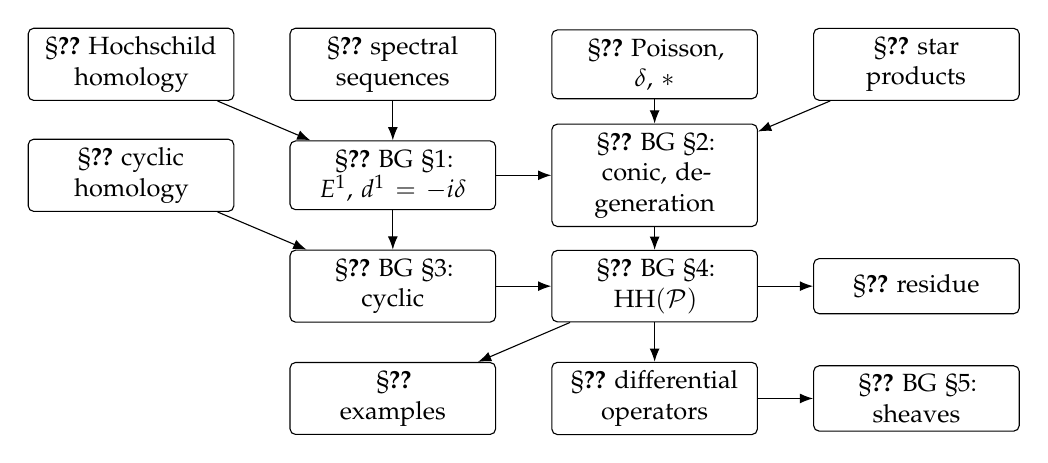
\begin{tikzpicture}[>=Latex,node distance=5mm and 7mm,
  box/.style={draw,rounded corners=2pt,align=center,font=\small,
  inner sep=3pt,minimum height=7mm,text width=24mm}]
 \node[box] (hh) {\S\ref{sec:HH} Hochschild\\ homology};
 \node[box,right=of hh] (ss) {\S\ref{sec:ss} spectral\\ sequences};
 \node[box,right=of ss] (po) {\S\ref{sec:poisson} Poisson,\\ \(\delta\), \(*\)};
 \node[box,right=of po] (st) {\S\ref{sec:star} star\\ products};
 \node[box,below=of ss] (b1) {\S\ref{sec:BG1} BG \S1:\\ \(E^1\), \(d^1=-i\delta\)};
 \node[box,right=of b1] (b2) {\S\ref{sec:BG2} BG \S2:\\ conic, degeneration};
 \node[box,left=of b1] (hc) {\S\ref{sec:HC} cyclic\\ homology};
 \node[box,below=of b1] (b3) {\S\ref{sec:BG3} BG \S3:\\ cyclic};
 \node[box,right=of b3] (sy) {\S\ref{sec:symbols} BG \S4:\\ \(\HH(\cP)\)};
 \node[box,right=of sy] (re) {\S\ref{sec:residue} residue};
 \node[box,below=of sy] (do) {\S\ref{sec:diffops} differential\\ operators};
 \node[box,right=of do] (sh) {\S\ref{sec:sheaf} BG \S5:\\ sheaves};
 \node[box,left=of do] (ex) {\S\ref{sec:examples}\\ examples};
 \draw[->] (hh)--(b1); \draw[->] (ss)--(b1); \draw[->] (po)--(b2);
 \draw[->] (st)--(b2); \draw[->] (b1)--(b2); \draw[->] (hc)--(b3);
 \draw[->] (b1)--(b3); \draw[->] (b2)--(sy); \draw[->] (sy)--(re);
 \draw[->] (b3)--(sy); \draw[->] (sy)--(do); \draw[->] (do)--(sh);
 \draw[->] (sy)--(ex);
\end{tikzpicture}
\caption[Logical structure of the notes]{Logical structure of the notes.
An arrow means ``is used by''. Appendix~\ref{app:connes} (Connes' theorem)
supports Section~\ref{sec:BG1}; Appendix~\ref{app:mixed} (the uncompleted
chain model) supports Section~\ref{sec:symbols}.}
\label{fig:roadmap}
\end{figure}

\subsection{How the notes follow BG}\label{subsec:follow}
Sections~\ref{sec:HH}--\ref{sec:star} are background. Then
\begin{center}
\begin{tabular}{ll}
\cite[\S1]{BG}, homology of quantum algebras & Section~\ref{sec:BG1}\\
\cite[\S2]{BG}, \(\delta\) on conic symplectic manifolds & Section~\ref{sec:BG2}\\
\cite[\S3]{BG}, cyclic homology of quantum algebras & Section~\ref{sec:BG3}\\
\cite[\S4]{BG}, symbols, residue, higher residues & Sections~\ref{sec:symbols}--\ref{sec:residue}\\
\cite[\S\S4--5]{BG}, differential operators & Section~\ref{sec:diffops}\\
\cite[\S5]{BG}, Poincaré lemmas and sheaves & Section~\ref{sec:sheaf}
\end{tabular}
\end{center}
Every statement of \cite{BG} that we use is restated, with its
hypotheses, before it is proved or quoted.

\section{Conventions, dictionary, quoted background and corrections}
\label{sec:conventions}

\begin{whatdoes}
We fix sign conventions, compatible with Loya's notes; give a dictionary
between the notation of \cite{BG}, of these notes and of Loya's notes; list
everything we quote without proof; and list our corrections to \cite{BG}.
\end{whatdoes}

\subsection{Conventions}\label{subsec:conv}
We follow \cite[\S``Pseudodifferential parametrices'']{LoyaAS}:
\(D_x=\frac1i\pa_x\), the left quantization
\[
 \Op(a)u(x)=(2\pi)^{-n}\int\!\!\int e^{i(x-y)\cdot\xi}a(x,\xi)u(y)\,dy\,d\xi ,
\]
and the composition formula \eqref{eq:intro-comp}. The symbol of \(D_{x_j}\) is
\(\xi_j\). On \(T^*M\), in canonical coordinates \((x,\xi)\), we use
\begin{gather*}
 \omega=\sum_{j=1}^n d\xi_j\wedge dx_j,\qquad
 \alpha=\sum_j\xi_j\,dx_j,\qquad d\alpha=\omega,\qquad
 \vol=\frac{\omega^n}{n!},\\
 \{a,b\}=\sum_j\Bigl(\frac{\pa a}{\pa\xi_j}\frac{\pa b}{\pa x_j}
 -\frac{\pa a}{\pa x_j}\frac{\pa b}{\pa\xi_j}\Bigr),\qquad
 H_a=\sum_j\Bigl(\frac{\pa a}{\pa\xi_j}\pa_{x_j}-\frac{\pa a}{\pa x_j}
 \pa_{\xi_j}\Bigr),\qquad \{a,b\}=H_ab .
\end{gather*}
Then \(\iota_{H_a}\omega=-da\). The radial vector field is
\(R=\sum_j\xi_j\pa_{\xi_j}\), and \(\iota_R\omega=\alpha\). The dilations
are \(\rho_t(x,\xi)=(x,t\xi)\), \(t>0\). A function or form \(\theta\) on
\(\Tdot M=T^*M\setminus0\) is \emph{homogeneous of degree} \(p\) if
\(\rho_t^*\theta=t^p\theta\); equivalently \(\Lie_R\theta=p\theta\). We
write \(\CI_{(p)}\) and \(\Om^k_{(p)}\) for these spaces. Note that \(dx_j\) has
degree \(0\), \(d\xi_j\) has degree \(1\) and \(\omega\) has degree \(1\).
With these conventions (Lemma~\ref{lem:commutator})
\[
 \sigma_{m+m'-1}([A,B])=-i\{\sigma_m(A),\sigma_{m'}(B)\}.
\]
The cosphere bundle \(S^*M=\Tdot M/\R_+\) is oriented by \(\iota_R\vol\)
(Lemma~\ref{lem:Sorient}). The circle is \(S^1=(0,\infty)/e^{\Z}\), the
radial half-line modulo integral dilations. All cohomology has complex
coefficients. Hochschild chains are \(C_k(A)=A^{\otimes(k+1)}\) (completed
when \(A\) is topological), and \(\HH_k\) is homology, never cohomology,
unless we say otherwise.

\subsection{Dictionary}\label{subsec:dictionary}
Table~\ref{tab:dictionary} compares notation. The most important
difference concerns Hamiltonian vector fields. BG write \(H_gf=\{f,g\}\),
so their \(H_g\) is our \(-H_g\). This changes the sign of some of their
formulas (Remark~\ref{rem:hamsign}).

\begin{table}[htbp]
\centering
\small
\renewcommand{\arraystretch}{1.15}
\begin{tabular}{>{\raggedright}p{3.6cm}>{\raggedright}p{5.2cm}>{\raggedright\arraybackslash}p{5.6cm}}
\hline
\cite{BG} & these notes & Loya's notes / standard\\
\hline
\(\Psi^\infty(M)\), \(\Psi^{-\infty}(M)\) & \(\Psi^{\Z}(M)\), \(\Psi^{-\infty}(M)\) & classical \(\Psi^m(M)\), smoothing operators\\
\(\cP=\Psi^\infty/\Psi^{-\infty}\) & \(\cP\), formal sums \(\sum_{j\le m}a_j\) & full symbols \(p\sim\sum p_{m-j}\)\\
\(\cP_c\) & \(\cP_c\) (\(M\) not compact) & compactly supported symbols\\
\(\Tdot M\), \(S^*M\) & \(\Tdot M=T^*M\setminus0\), \(S^*M\) & cotangent and cosphere bundles\\
\(a\star b\), \(\varphi_i\) & \(a\star b=\sum_lP_l(a,b)\) & \(p\#q\), composition formula\\
\(\hb\), \(A\{\hb\}\), \(\C\{\hb\}\) & \(\hb\), \(A\Lser{\hb}\), \(K=\C\Lser{\hb}\) & semiclassical parameter\\
\(\{f,g\}\), \(H_gf=\{f,g\}\) & \(\{a,b\}=H_ab\), so \(H^{\mathrm{BG}}_g=-H_g\) & \(\sigma([P,Q])=-i\{p,q\}\)\\
\(\omega\), \(\omega^{-1}\) & \(\omega=\sum d\xi_j\wedge dx_j\), bivector \(\pi\) & symplectic form\\
\(\mathcal R\), \(T_t\) & \(R=\sum\xi_j\pa_{\xi_j}\), \(\rho_t\) & homogeneity in \(\xi\)\\
\(\eps(v)\), \(\eps^*(v)\), \(\iota^*(Z)\) & \(\eps(\theta)\), \(\iota_{\pi^\sharp\theta}\), \(\eps(\iota_Z\omega)\) & exterior and interior products\\
\(*\) (an \(\mathfrak{sl}(2)\) exponential) & \(*\), \(\alpha\wedge*\beta=\Lambda(\alpha,\beta)\vol\) & analogue of the Hodge star\\
\(\delta\) (Koszul) & \(\delta=[\iota_\pi,d]=\iota_\pi d-d\iota_\pi\) & Poisson ``codifferential''\\
\(b\), \(B\), \(u\) & \(b\), \(B\), \(u\) & Hochschild and Connes operators\\
\(E^i_{kl}\) (\(k\) form degree, \(l\) homogeneity) & \(E^r_{p,k}\) (\(p\) order, \(k\) degree) & spectral sequence pages\\
\(R(P)\) & \(\res\) & Wodzicki--Guillemin residue\\
\(\mathrm{Res}_m\) & higher residue functionals & Wodzicki's higher residues\\
\(\cD(M)\), \(\cD_M\) & \(\cD(M)\), sheaf \(\cD_M\) & differential operators\\
\(\cE\), \(\cE^\infty\), \(\cE_{\R}\) & same (quoted, Section~\ref{subsec:micro}) & microdifferential operators\\
\(H^*(X)\{\hb\}\) & \(H^*(X)\Lser{\hb}\) & Laurent series in \(\hb\)\\
\hline
\end{tabular}
\caption{Dictionary of notation.}
\label{tab:dictionary}
\end{table}

\subsection{Quoted background}\label{subsec:quoted}
The following facts are used without proof. Every place where one of them
is used names it. Everything else is proved in these notes.
\begin{enumerate}
\item[(G1)] \emph{Classical pseudodifferential calculus}
\cite{LoyaAS,Hormander3,MelroseMicro}. On a manifold \(M\), compact or not:
(a) in a chart, the left quantization identifies operators of order \(m\)
with compactly supported kernels, modulo \(\Psi^{-\infty}\), with
classical symbols of order \(m\) modulo \(S^{-\infty}\), and every formal
sum of homogeneous terms is the expansion of a symbol (Borel's lemma);
(b) the full symbol of a product is given by \eqref{eq:intro-comp} modulo
\(S^{-\infty}\); (c) under a change of coordinates the full symbol
transforms by a formal series of differential operators, each lowering
the degree of homogeneity, whose top term is the pull-back of the
principal symbol; (d) Schwartz kernels are smooth off the diagonal, so
an operator \(\phi A\psi\) with \(\supp\phi\cap\supp\psi=\varnothing\) is
smoothing; (e) an elliptic element of \(\cP\) (one with invertible principal
symbol) is invertible in \(\cP\), by the parametrix construction of
\cite[\S``Pseudodifferential parametrices'']{LoyaAS}; this is used for the operator
\(T\) of Appendix~\ref{app:mixed}. We prove the further consequence, the global
star product, in Proposition~\ref{prop:globalstar}.
\item[(G2)] \emph{Nuclear spaces} \cite[Chs.~43, 50, 51]{Treves}. For
manifolds \(X\), \(Y\), \(\CI(X)\hot\CI(Y)=\CI(X\times Y)\), where \(\hot\) is
the completed projective tensor product. The functor \(E\hot(\cdot)\), for
\(E\) nuclear Fréchet, is exact on Fréchet spaces and commutes with
countable products.
\item[(G3)] \emph{Eilenberg--Zilber theorem} \cite[\S4.2]{Loday},
\cite[\S8.5]{Weibel}: the shuffle map from the tensor product of two
Hochschild complexes of unital algebras to the Hochschild complex of the
tensor product is a chain homotopy equivalence, given by universal finite
formulas.
\item[(G4)] \emph{Basic homological algebra} \cite[Chs.~2, 3, 5]{Weibel}: the
comparison theorem for projective resolutions; Künneth over a field;
the general construction of the pages \(E^r\) of a filtered complex.
\item[(G5)] \emph{Algebraic topology and Hodge theory} \cite{BottTu,LoyaAS}:
de Rham's theorem, Poincaré duality, the Künneth formula, the Gysin
sequence, Hodge theory on the round sphere (a continuous Green operator
for the Laplacian), and Weil's theorem in the general form of
Background~\ref{bg:weil}.
\item[(G6)] \emph{Darboux theorems} \cite{CannasdaSilva},
\cite[\S21.1]{Hormander3}: local Darboux coordinates on a symplectic
manifold, and the homogeneous version on a conic symplectic manifold.
\item[(G7)] \emph{De Wilde--Lecomte} \cite{deWildeLecomte}: existence and
uniqueness of local conic star products, in the form of
Background~\ref{bg:dWL}.
\item[(G8)] \emph{Trace class and complex powers} \cite{Seeley,Shubin}:
operators of order \(<-n\) are of trace class with trace given by the
integral of the kernel on the diagonal, and Seeley's complex powers form
a holomorphic family (Background~\ref{bg:seeley}).
\item[(G9)] \emph{H-unitality, excision and Morita invariance}
\cite{Wodzicki-excision,Loday}: \(\CI_c(M)\) and \(\Psi^{-\infty}(M)\) are H-unital;
an H-unital ideal gives a long exact sequence in Hochschild homology; and
\(\HH_*(\Psi^{-\infty}(M))\cong\HH_*(\C)\). These are used only in remarks.
\item[(G10)] \emph{The Milnor sequence} \cite[\S3.5]{Weibel}: for a tower of
complexes with surjective maps, \(0\to\varprojlim^1H_{k+1}\to H_k(\varprojlim)\to\varprojlim H_k\to0\). It is
used for periodic cyclic homology and in the discussion of BG's convergence
argument (Remark~\ref{rem:convergence}).
\item[(G11)] \emph{HKR for fibrewise polynomial functions on \(T^*M\)}. It
is used only for differential operators on a general manifold
(Theorem~\ref{thm:DM}); we prove it when \(M\) is an open subset of \(\R^n\).
\item[(G12)] \emph{Sheaf theory} \cite{BottTu,Bredon}: sheafification,
hypercohomology, and the localization of Hochschild complexes of sheaves
of algebras \cite{Teleman,Brylinski-examples}. It is used in
Section~\ref{sec:sheaf} only.
\item[(G13)] \emph{Microlocal analysis} \cite{SKK,Kashiwara-book,KashiwaraKawai,Brylinski-examples}:
the sheaves \(\cE\), \(\cE^\infty\), \(\cE_{\R}\) and the four results listed
in Background~\ref{bg:micro}; also the existence of a real-analytic structure on
every smooth manifold, compatible with its smooth structure (Whitney), and of a
complexification \(M\hookrightarrow M_{\C}\). They are used in Section~\ref{subsec:micro}
only.
\item[(G14)] \emph{Algebraic de Rham theory}: Grothendieck's comparison
theorem \cite{Grothendieck}, the Lefschetz principle, and the proposition of
Kassel and Mitschi \cite{KasselMitschi} (Background~\ref{bg:KM}), quoted by
BG from a private communication.
\item[(G15)] \emph{Results quoted for comparison only}: the computation of
Hochschild homology of deformation quantizations of general symplectic
manifolds by Nest and Tsygan \cite{NestTsygan}, and Wodzicki's computations
\cite{Wodzicki-residue,Wodzicki-cyclic}.
\end{enumerate}
Connes' theorem \(\HH_k(\CI(M))\cong\Om^k(M)\) is \emph{proved}, in
Appendix~\ref{app:connes}, for manifolds without boundary, compact or not.

\subsection{Corrections and remarks on BG}\label{subsec:corrections}
The points where we disagree with the text of \cite{BG}, or where
hypotheses are left implicit, are the following. Each is discussed and
verified at the place indicated.
\begin{enumerate}
\item \emph{Sign in the formula for \(\delta\).} The second sum in
\cite[\S1, Thm.~(2), and \S2]{BG} should carry \((-1)^{i+j}\), not
\((-1)^{i+j+1}\). As printed the operator is not well defined on forms
(Correction~\ref{corr:delta}).
\item \emph{Normalization of \(d^1\) and of \(B\).} The constant
\(\hb/i\) in \(d^1=(\hb/i)\delta\) holds for the HKR map normalized by
\(1/k!\). With the identification drawn in BG's diagram it becomes
\(\hb/(ik)\) on \(k\)-forms, and \(B\) becomes \((k+1)d\)
(Correction~\ref{corr:normalization}).
\item \emph{The \(\mathfrak{sl}(2)\) star operator.} BG's data are internally
inconsistent: with their relations the operator
\(\exp(\frac{\pi i}2(\eps(\omega)+\eps^*(\omega)))\) is not of finite order, and the matrix
identity used to prove \(*^2=1\) is false (the exponential is \(-1\)). The consistent
fix is to drop the factor \(i\), which gives \(*^2=(-1)^{d-1}\) on irreducible
\(\mathfrak{sl}(2)\)-components of dimension \(d\). The conclusions hold up to non-zero
constants (Correction~\ref{corr:sl2}).
\item \emph{The ``in particular'' of the main theorem.} The claim
\(\HH_*(\cP)\cong H^{n-*-1}(M)\oplus H^{n-*}(M)\) for \(n>1\) in
\cite[\S4, Thm.~(1)]{BG}, stated for general \(M\) (and for \(\cP_c\)), is false. It
fails for \(M=S^2\), and also when the Euler class vanishes: for \(M=T^2\) and \(k=0\)
it gives \(\C^3\) instead of \(\C\). It contradicts BG's own \(\HH_0(\cP)\cong\C\) whenever
\(b_{n-1}(M)\ne0\). A correct description, valid when the Euler class vanishes, comes
from the Gysin sequence (Correction~\ref{corr:gysin}).
\item \emph{The filtration for cyclic homology.} The filtration
\(F_m(\cP[u])=\sum_ju^jF_{m+2j}(\cP)\) of \cite[\S4]{BG} is not preserved
by \(u^{-1}B\). It should be \(\sum_ju^jF_{m-2j}(\cP)\)
(Correction~\ref{corr:cyclicfilt}).
\item \emph{The zeta-function constant.} In \cite[\S4, Prop.~(2)]{BG}
the constant in \(\Res_{s=0}\Tr(PA^{-s})=c\,R(P)\) depends on the order
\(m\) of \(A\): it is proportional to \(1/m\). The assertion ``\(c=2\pi\)'' at the end of the
proof of Prop.~(1) is unclear, and under either reading we obtain a different
constant (Correction~\ref{corr:zeta}).
\item \emph{Quantum algebras.} BG never specify the quantization used for
\(\cP\), and the parity condition \(\varphi_i(a,b)=(-1)^i\varphi_i(b,a)\) is never used (it
fails, for instance, for the left-quantized product). Also
\(a\star b-b\star a=(\hb/i)\{a,b\}\) holds only up to \(O(\hb^3)\)
(Remark~\ref{rem:parity}).
\item \emph{Darboux and the conic structure.} BG's conic Darboux lemma does not
say that the symplectomorphism commutes with the dilations, which is what is
used; its image is an open conic subset of \(\Tdot\R^n\). The flow is \(T_t=\exp((\log t)\mathcal R)\), not \(\exp(t\mathcal R)\)
(Remark~\ref{rem:darboux}).
\item \emph{Convergence.} The convergence argument in \cite[\S\S2,4]{BG}
appeals to Mittag-Leffler without the required estimates, and it depends
on the completion used for the chains. We prove convergence for two chain
models and show that they give the same homology
(Remark~\ref{rem:convergence}).
\item \emph{Higher residues.} The cochain \(T\alpha\) of \cite[\S4]{BG} is
defined by a leading-order formula and is not shown to be a Hochschild
cocycle. We give the precise statement, as a functional on \(\HH_m(\cP)\)
(Remark~\ref{rem:higherres}).
\item \emph{Hypotheses.} Uniqueness of the residue needs \(M\) connected
and \(n\ge2\) (BG say so in the text, not in the proposition). Statements
for non-compact \(M\) concern \(\cP_c\) and compactly supported
cohomology (Remark~\ref{rem:hyp}).
\item \emph{Sheaf-theoretic gaps.} In \cite[\S5]{BG} the presheaf
\(U\mapsto C_k(\cD(U))\) is not a presheaf of the kind that Weil's
argument needs without a localization step, and the splitting argument
for cyclic homology is stated with the arrows reversed. Both points are
fixed in Remark~\ref{rem:sheafgap}.
\item \emph{Misprints.} The upper limit \(n\) for \(m\) in the formula for
\(\delta\) in \S2; \(\alpha=\iota(\omega)\) for \(\iota(\mathcal R)\omega\) in
\S4; the index \(k\) for \(q\) in the Poincaré lemma of \S5; the words
``convergence'' and ``degeneration'' exchanged in the proof of the theorem
of \S3; ``Hochschild cohomology'' for homology at the start of \S5; and
``\(m\) sufficiently large'' for ``\(-m\) sufficiently large'' in \S4. We
note these where they occur.
\end{enumerate}

\section{Hochschild homology for beginners}\label{sec:HH}

\begin{whatdoes}
We define Hochschild homology, starting from its degree-zero part, which
is the space dual to traces. We compute it for polynomial rings and for the
Weyl algebra by hand, prove the Hochschild--Kostant--Rosenberg theorem for
polynomial algebras, and state Connes' theorem for smooth functions.
Everything except Section~\ref{subsec:topological} is pure algebra over
\(\C\).
\end{whatdoes}

Throughout, \(A\) is an associative algebra over \(\C\) with unit \(1\),
unless we say otherwise.

\subsection{Degree zero: traces}\label{subsec:HH0}
Let \([A,A]\) be the linear span of all commutators \([a,b]=ab-ba\).

\begin{definition}
\(\HH_0(A)=A/[A,A]\). A \emph{trace} on \(A\) is a linear map
\(\tau:A\to\C\) with \(\tau(ab)=\tau(ba)\) for all \(a,b\).
\end{definition}

A linear functional is a trace exactly when it vanishes on \([A,A]\), so
traces are the same thing as linear functionals on \(\HH_0(A)\). Finding all
traces on an algebra is therefore the problem of computing \(\HH_0\).

\begin{example}[Matrices]\label{ex:matrices}
For \(A=M_N(\C)\) with matrix units \(E_{ij}\), we have \(E_{ij}=[E_{ik},E_{kj}]\)
for \(i\ne j\) (any \(k\)), and \(E_{ii}-E_{jj}=[E_{ij},E_{ji}]\). So \([A,A]\)
contains the matrices of trace zero, and \(\HH_0(M_N(\C))\cong\C\), via the
usual trace.
\end{example}

\begin{example}[Commutative algebras]
If \(A\) is commutative then \([A,A]=0\) and \(\HH_0(A)=A\).
\end{example}

\begin{example}[The Weyl algebra has no traces]\label{ex:weylHH0}
Let \(A_1\) be the algebra of differential operators on \(\R\) with
polynomial coefficients. It is spanned by \(x^a\pa^b\), \(a,b\ge0\), and
\([\pa,x^{a+1}\pa^b]=(a+1)x^a\pa^b\). So every element is a commutator
and \(\HH_0(A_1)=0\). There is no non-zero trace on \(A_1\).
\end{example}

\begin{example}[Symbols: a preview]\label{ex:symbolpreview}
In \(\cP(\R^n)\) restricted to symbols with compact \(x\)-support the same
idea works partially. In the left quantization (Lemma~\ref{lem:xDcomm})
\[
 [x_k,\Op(a)]=i\Op(\pa_{\xi_k}a),\qquad [D_{x_k},\Op(a)]=\Op(D_{x_k}a).
\]
So every \(\xi\)-derivative and every \(x\)-derivative of a symbol is a
commutator. By Euler's identity, a function \(a_j\) homogeneous of degree
\(j\) satisfies \(\sum_k\pa_{\xi_k}(\xi_ka_j)=(j+n)a_j\). Hence every term
of degree \(j\ne-n\) is a commutator, and only the term \(a_{-n}\) can
survive in \(\HH_0\). This is the origin of the residue. We return to it
in Section~\ref{sec:residue}.
\end{example}

\subsection{Degree one: differential forms}\label{subsec:HH1}
To go further we need the chains of degree one and two:
\[
 C_1(A)=A\otimes A\xrightarrow{\;b\;}C_0(A)=A,\qquad b(a_0\otimes a_1)=a_0a_1-a_1a_0,
\]
\[
 C_2(A)=A^{\otimes3}\xrightarrow{\;b\;}C_1(A),\qquad
 b(a_0\otimes a_1\otimes a_2)=a_0a_1\otimes a_2-a_0\otimes a_1a_2+a_2a_0\otimes a_1 .
\]
One checks \(b\circ b=0\) on \(C_2\) directly; the general case is
Lemma~\ref{lem:bb}. Then \(\HH_0=A/b(C_1)\), and
\(\HH_1(A)=\ker(b:C_1\to C_0)/b(C_2)\).

For a commutative algebra \(A\), the module of \emph{Kähler differentials}
\(\Om^1_A\) is the \(A\)-module generated by symbols \(db\), \(b\in A\),
subject to linearity in \(b\) and the Leibniz rule \(d(bc)=b\,dc+c\,db\).
For \(A=\C[x_1,\dots,x_n]\) it is the free module on \(dx_1,\dots,dx_n\),
and for smooth functions on a manifold it maps onto the ordinary
\(1\)-forms.

\begin{proposition}\label{prop:HH1}
If \(A\) is commutative, \(a_0\otimes a_1\mapsto a_0\,da_1\) induces an
isomorphism \(\HH_1(A)\cong\Om^1_A\).
\end{proposition}

\begin{proof}
Since \(A\) is commutative, \(b=0\) on \(C_1\), so every \(1\)-chain is a
cycle. The map kills boundaries:
\[
 b(a_0\otimes a_1\otimes a_2)\mapsto a_0a_1\,da_2-a_0\,d(a_1a_2)+a_2a_0\,da_1=0
\]
by the Leibniz rule. Conversely, define \(\Om^1_A\to\HH_1(A)\) by
\(a\,db\mapsto[a\otimes b]\). It respects the relations, because
\[
 a\otimes bc-ab\otimes c-ac\otimes b=-b(a\otimes b\otimes c),
\]
and it is \(A\)-linear for the module structure \(c\cdot[a\otimes b]=[ca\otimes b]\)
by construction. The two maps are inverse to each other.
\end{proof}

So \(\HH_1(\C[x])\cong\C[x]\,dx\). In Section~\ref{subsec:barres} we show that
\(\HH_k(\C[x])=0\) for \(k\ge2\), and in Section~\ref{subsec:HKR} that
\(\HH_k\) of a polynomial ring is the space of \(k\)-forms. The slogan is:
\emph{for commutative algebras, Hochschild homology is differential forms.}

\subsection{The Hochschild complex}\label{subsec:complex}
\begin{definition}\label{def:hochschild}
The Hochschild chains are \(C_k(A)=A^{\otimes(k+1)}\), \(k\ge0\). The
\emph{face maps} \(d_i:C_k\to C_{k-1}\), \(0\le i\le k\), are
\[
 d_i(a_0\otimes\dots\otimes a_k)=a_0\otimes\dots\otimes a_ia_{i+1}\otimes
 \dots\otimes a_k\quad(i<k),\]
\[
 d_k(a_0\otimes\dots\otimes a_k)=a_ka_0\otimes a_1\otimes\dots\otimes a_{k-1}.
\]
The Hochschild boundary is \(b=\sum_{i=0}^k(-1)^id_i\), and the bar
boundary is \(b'=\sum_{i=0}^{k-1}(-1)^id_i\). Hochschild homology is
\(\HH_k(A)=H_k(C_\bullet(A),b)\).
\end{definition}

\begin{lemma}\label{lem:bb}
\(d_id_j=d_{j-1}d_i\) for \(i<j\). Consequently \(b^2=0\) and \(b'^2=0\).
\end{lemma}

\begin{proof}
The identity is a statement about which adjacent entries are multiplied
first; for \(i<j-1\) the two products are in different places, and for
\(i=j-1\) it is associativity. When \(j=k\) and \(i=0\) both sides give
\(a_ka_0a_1\otimes\cdots\), again by associativity. Then
\(b^2=\sum_{i,j}(-1)^{i+j}d_id_j\), and the terms with \(i<j\) cancel
against the terms \(d_{j-1}d_i\) with indices \((j-1,i)\), \(j-1\ge i\),
which have the opposite sign. The same argument applies to \(b'\).
\end{proof}

Picture an elementary chain \(a_0\otimes\dots\otimes a_k\) as \(k+1\) beads
on a circle. The face \(d_i\) multiplies neighbouring beads \(i\) and
\(i+1\), and \(d_k\) closes the necklace by multiplying the last bead with
the first. The cyclic nature of \(d_k\) is why traces appear in degree zero.

\subsection{The bar resolution and small resolutions}\label{subsec:barres}
\emph{This subsection uses a little homological algebra and can be skimmed on a
first reading; its only output used later is Example~\ref{ex:Cx} and the proof of
Theorem~\ref{thm:HKRpoly}.} Here is what is needed. A module is \emph{free} if it has
a basis. A \emph{free resolution} of a module \(N\) is an exact sequence
\(\cdots\to P_1\to P_0\to N\to0\) with every \(P_k\) free; think of it as a presentation of
\(N\) by generators (\(P_0\)), relations (\(P_1\)), relations between relations, and so on.
If \(P_\bullet\to N\) is a free resolution of a right \(R\)-module and \(L\) is a left
\(R\)-module, the homology of the complex \(P_\bullet\otimes_RL\) is called
\(\Tor^R_\bullet(N,L)\). The \emph{comparison theorem} (G4) says that any two free (or
projective) resolutions of \(N\) are chain homotopy equivalent, by maps covering the
identity of \(N\), so \(\Tor\) does not depend on the resolution. In practice: to
compute \(\Tor\), choose the smallest resolution you can find. We apply this with
\(R=A^e\), \(N=L=A\).

Let \(A^e=A\otimes A^{\mathrm{op}}\). An \(A\)-bimodule is the same thing as a
left \(A^e\)-module, with \((a\otimes b)\cdot m=amb\). Put
\(B_k(A)=A\otimes A^{\otimes k}\otimes A\) (free \(A^e\)-modules), with the
bar boundary \(b'\).

\begin{lemma}\label{lem:barres}
\(\cdots\to B_1\xrightarrow{b'}B_0=A\otimes A\xrightarrow{\mu}A\to0\),
where \(\mu\) is multiplication, is exact; it is a free resolution of \(A\)
as an \(A^e\)-module. Moreover \(A\otimes_{A^e}B_k\cong C_k(A)\), and the
induced differential is \(b\).
\end{lemma}

\begin{proof}
The map \(s(a_0\otimes\dots\otimes a_{k+1})=1\otimes a_0\otimes\dots\otimes
a_{k+1}\) satisfies \(b's+sb'=1\), because \(d_0s=1\) and \(d_{i+1}s=sd_i\).
A complex with such a contraction is exact. The isomorphism is
\(a\otimes_{A^e}(a_0\otimes w\otimes a_{k+1})\mapsto a_{k+1}aa_0\otimes w\),
and under it the last face of \(b'\) becomes the cyclic face \(d_k\).
\end{proof}

So \(\HH_k(A)=\Tor_k^{A^e}(A,A)\). By the comparison theorem of homological
algebra (G4), \emph{any} projective resolution \(P_\bullet\to A\) by
\(A^e\)-modules computes the same homology after applying
\(A\otimes_{A^e}(\cdot)\). Small resolutions give quick computations.

\begin{example}[Polynomials and Laurent polynomials in one variable]
\label{ex:Cx}
Let \(A=\C[x]\), so \(A^e=\C[x,y]\). The sequence
\[
 0\to A^e\xrightarrow{\,(x-y)\,}A^e\xrightarrow{\,f(x,y)\mapsto f(x,x)\,}A\to0
\]
is exact: \(x-y\) is not a zero divisor, and \(f(x,y)-f(x,x)\) is divisible by
\(x-y\). Applying \(A\otimes_{A^e}\cdot\) sets \(y=x\), and the map \(x-y\)
becomes \(0\). Hence \(\HH_0(\C[x])=\C[x]\), \(\HH_1(\C[x])=\C[x]\), which is
\(\C[x]\,dx\) by Proposition~\ref{prop:HH1}, and \(\HH_k(\C[x])=0\) for \(k\ge2\).
The same holds for \(A=\C[r,r^{-1}]\): after clearing a denominator
\((rs)^N\), \(f(r,s)-f(r,r)\) is divisible by \(r-s\). Thus
\(\HH_1(\C[r^{\pm1}])=\C[r^{\pm1}]\,dr\), and \(\HH_k=0\) for \(k\ge2\).
\end{example}

\subsection{The Hochschild--Kostant--Rosenberg theorem}\label{subsec:HKR}
For a commutative algebra define the \emph{HKR map} and the
\emph{antisymmetrization}
\begin{equation}\label{eq:HKR}
 \chi(a_0\otimes\dots\otimes a_k)=\frac1{k!}\,a_0\,da_1\wedge\dots\wedge da_k,
 \qquad
 \operatorname{Alt}(a_0;a_1,\dots,a_k)=\sum_{\sigma\in\mathfrak S_k}\sgn(\sigma)\,
 a_0\otimes a_{\sigma(1)}\otimes\dots\otimes a_{\sigma(k)} .
\end{equation}
The factor \(1/k!\) is a normalization; it matters for the constants in
Section~\ref{sec:BG1} (Correction~\ref{corr:normalization}).

\begin{lemma}\label{lem:chi}
For a commutative algebra, \(\chi\circ b=0\), \(b\circ\operatorname{Alt}=0\), and
\(\chi\operatorname{Alt}(a_0;a_1,\dots,a_k)=a_0\,da_1\wedge\dots\wedge da_k\).
\end{lemma}

\begin{proof}
Write \(T_i=a_0a_i\,da_1\wedge\dots\widehat{da_i}\dots\wedge da_k\). We
compute \((k-1)!\,\chi(b(a_0\otimes\dots\otimes a_k))\) face by face. The
face \(d_0\) gives \(a_0a_1\,da_2\wedge\dots\wedge da_k=T_1\). For
\(1\le i\le k-1\) the face \(d_i\) gives
\(a_0\,da_1\wedge\dots\wedge d(a_ia_{i+1})\wedge\dots\wedge da_k\), and the
Leibniz rule \(d(a_ia_{i+1})=a_i\,da_{i+1}+a_{i+1}\,da_i\) turns this into
\(T_i+T_{i+1}\). The face \(d_k\) gives \(a_ka_0\,da_1\wedge\dots\wedge
da_{k-1}=T_k\). Hence
\[
 (k-1)!\,\chi\bigl(b(a_0\otimes\dots\otimes a_k)\bigr)=T_1+\sum_{i=1}^{k-1}
 (-1)^i(T_i+T_{i+1})+(-1)^kT_k .
\]
The coefficient of \(T_1\) is \(1-1=0\), that of \(T_j\) for \(2\le j\le k-1\)
is \((-1)^{j-1}+(-1)^j=0\), and that of \(T_k\) is
\((-1)^{k-1}+(-1)^k=0\). For \(b\operatorname{Alt}\): the inner faces cancel in pairs,
\(\sigma\) against \(\sigma\circ(i\ i{+}1)\), because the algebra is
commutative; and the face \(d_0\) for \(\sigma\) cancels \((-1)^kd_k\) for the
cyclically shifted permutation, whose sign is \((-1)^{k-1}\sgn\sigma\). The
third identity holds because each of the \(k!\) terms of \(\operatorname{Alt}\)
contributes \(\frac1{k!}a_0\,da_1\wedge\dots\wedge da_k\) after reordering
the wedge product.
\end{proof}

\begin{theorem}[Hochschild--Kostant--Rosenberg for polynomial algebras \cite{HKR}]
\label{thm:HKRpoly}
Let \(A=\C[x_1,\dots,x_n]\). Then \(\chi\) induces isomorphisms
\(\HH_k(A)\cong\Om^k_A=A\otimes\Lambda^k\C^n\), with inverse
\(a_0\,dx_{i_1}\wedge\dots\wedge dx_{i_k}\mapsto[\operatorname{Alt}(a_0;x_{i_1},\dots,x_{i_k})]\).
\end{theorem}

\begin{proof}
\emph{The Koszul resolution.} Identify \(A^e=\C[x,y]\), with \(x\) acting on
the left and \(y\) on the right. Let \(K_k=A^e\otimes\Lambda^k\C^n\), with
basis \(e_{i_1}\wedge\dots\wedge e_{i_k}\), and
\[
 \pa(f\,e_{i_1}\wedge\dots\wedge e_{i_k})=\sum_{j=1}^k(-1)^{j-1}(x_{i_j}-y_{i_j})
 f\,e_{i_1}\wedge\dots\widehat{e_{i_j}}\dots\wedge e_{i_k},
\]
augmented by \(K_0=A^e\to A\), \(f\mapsto f(x,x)\). In the variables
\(w=x-y\), \(v=y\), \(\pa\) is contraction with \(\sum_iu_i\,\pa/\pa e_i\).
Let \(h(f\,e_I)=\sum_i\frac{\pa f}{\pa w_i}e_i\wedge e_I\). Then
\(\pa h+h\pa\) multiplies \(f\,e_I\) by (degree of \(f\) in \(w\)) \(+|I|\),
the usual Euler identity. So \(K\) is exact except in degree \(0\), where
the homology is \(\C[v]\cong A\) through \(f\mapsto f(x,x)\). Thus \(K\) is a
free resolution of \(A\).

\emph{Comparison.} The map \(\Phi(e_{i_1}\wedge\dots\wedge e_{i_k})=
\sum_\sigma\sgn\sigma\,1\otimes x_{i_{\sigma(1)}}\otimes\dots\otimes
x_{i_{\sigma(k)}}\otimes1\), extended \(A^e\)-linearly, is a chain map
\(K\to B(A)\) over the identity of \(A\): in \(b'\Phi\) the inner faces cancel
in pairs, and the two outer faces give
\(\sum_l(-1)^{l-1}(x_{i_l}\otimes1-1\otimes x_{i_l})\) times the shorter
antisymmetrization. By the comparison theorem it induces an isomorphism
on homology after \(A\otimes_{A^e}\). On the Koszul side
\(A\otimes_{A^e}K=A\otimes\Lambda\C^n\) with zero differential, since
\(x_i-y_i\) acts as \(0\). On the Hochschild side \(\Phi\) becomes
\(a_0\,e_I\mapsto\operatorname{Alt}(a_0;x_{i_1},\dots,x_{i_k})\). So the classes
\(\operatorname{Alt}(a_0;x_{i_1},\dots,x_{i_k})\) form a basis of \(\HH_k(A)\) over
the basis of \(A\otimes\Lambda^k\), and \(\chi\operatorname{Alt}=\mathrm{id}\) by
Lemma~\ref{lem:chi}.
\end{proof}

\subsection{The Weyl algebra: a first Poincaré lemma}\label{subsec:weyl}
The \emph{Weyl algebra} \(A_n\) is the algebra of differential operators on
\(\R^n\) with polynomial coefficients. It is generated by \(x_i\) and
\(\pa_i=\pa/\pa x_i\), with \([\pa_i,x_j]=\delta_{ij}\) and all other
generators commuting. Normal ordering \(x^\alpha\pa^\beta\mapsto
x^\alpha\xi^\beta\) is a linear isomorphism \(A_n\cong\C[x,\xi]\).

\begin{theorem}[Feigin--Tsygan \cite{FeiginTsygan}; Wodzicki]\label{thm:weyl}
\(\HH_k(A_n)\cong\C\) for \(k=2n\), and \(\HH_k(A_n)=0\) otherwise.
\end{theorem}

This is the ``Poincaré lemma'' of \cite[\S5]{BG} for polynomial
coefficients: \(\HH_*(A_n)\cong H^{2n-*}(\R^n)\). The proof is elementary.

\begin{proof}
\emph{Commuting elements of \(A^e\).} In \(A^e=A_n\otimes A_n^{\mathrm{op}}\)
put \(U_i=x_i\otimes1-1\otimes x_i\) and \(V_i=\pa_i\otimes1-1\otimes\pa_i\).
In \(A^{\mathrm{op}}\) the commutator is reversed, so \([1\otimes x_i,1\otimes\pa_j]
=1\otimes(\pa_jx_i-x_i\pa_j)=\delta_{ij}\), while \([x_i\otimes1,\pa_j\otimes1]=
-\delta_{ij}\). Hence \([U_i,V_j]=-\delta_{ij}+\delta_{ij}=0\), and the
\(2n\) elements \(W=(U_1,\dots,U_n,V_1,\dots,V_n)\) commute.

\emph{The Koszul resolution.} Let \(K_k=A^e\otimes\Lambda^k\C^{2n}\) with
\(\pa(c\otimes e_I)=\sum_j(-1)^{j-1}cW_{i_j}\otimes e_{I\setminus i_j}\) (right
multiplication, so \(\pa\) is \(A^e\)-linear for the left action), augmented by
\(c\mapsto c\cdot1\), that is \(a\otimes b\mapsto ab\). Since the \(W_i\)
commute, \(\pa^2=0\). Filter \(A^e\) by total degree in all generators (the
Bernstein filtration). The associated graded algebra is the polynomial ring
\(\C[x,\xi,y,\eta]\) in \(4n\) variables, and the \(W_i\) have leading terms
\(x_i-y_i\), \(\xi_i-\eta_i\). The associated graded complex of \(K\) is the
Koszul complex of these linear forms, which is exact except in degree
\(0\) by the proof of Theorem~\ref{thm:HKRpoly} (change variables to
\(u=(x-y,\xi-\eta)\)). Its \(H_0\) is \(\C[x,\xi]=\gr A_n\). A complex with an
exhaustive filtration, bounded below, whose associated graded complex is
exact, is itself exact: a cycle of filtration degree \(N\) is a boundary
modulo filtration degree \(N-1\), and we induct on \(N\). Hence \(K\) is a free
resolution of \(A_n\).

\emph{The Koszul complex of \(A_n\).} Applying \(A_n\otimes_{A^e}\) gives
\(A_n\otimes\Lambda\C^{2n}\), with differential
\(\pa(a\,e_I)=\sum_j(-1)^{j-1}(a\cdot W_{i_j})\,e_{I\setminus i_j}\), where
\(A^e\) acts on the right of \(A_n\) by \(a\cdot(p\otimes q)=qap\). Thus
\(a\cdot U_i=-[x_i,a]\) and \(a\cdot V_i=-[\pa_i,a]\). In normal ordering,
\([\pa_i,x^\alpha\pa^\beta]=\alpha_ix^{\alpha-e_i}\pa^\beta\) and
\([x_i,x^\alpha\pa^\beta]=-\beta_ix^\alpha\pa^{\beta-e_i}\). So, with
\(y=(\xi,-x)\in\C^{2n}\) as coordinates on \(\C[x,\xi]\cong A_n\), the complex
is \(\C[y_1,\dots,y_{2n}]\otimes\Lambda\C^{2n}\) with
\(\pa=\sum_i\frac{\pa}{\pa y_i}\iota_i\), where \(\iota_i\) is contraction with
the \(i\)-th dual basis vector, \(\iota_i(e_{i_1}\wedge\dots\wedge e_{i_k})=
\sum_j(-1)^{j-1}\delta_{i,i_j}e_{I\setminus i_j}\).

\emph{The polynomial Poincaré lemma.} Let \(\eps_i\) be exterior
multiplication by \(e_i\) and \(h=\sum_iy_i\eps_i\). Since
\(\frac{\pa}{\pa y_i}y_j=y_j\frac{\pa}{\pa y_i}+\delta_{ij}\) and
\(\iota_i\eps_j+\eps_j\iota_i=\delta_{ij}\),
\[
 \pa h+h\pa=\sum_{i,j}y_j\frac{\pa}{\pa y_i}(\iota_i\eps_j+\eps_j\iota_i)
 +\sum_i\iota_i\eps_i=\sum_iy_i\frac{\pa}{\pa y_i}+\sum_i\iota_i\eps_i .
\]
On \(f\,e_I\) with \(f\) homogeneous this is multiplication by
\(\deg f+(2n-|I|)\), which is invertible unless \(f\) is constant and
\(|I|=2n\). Hence the homology is \(\C\,e_1\wedge\dots\wedge e_{2n}\), in
degree \(2n\).
\end{proof}

\begin{example}[An explicit generator of \(\HH_2(A_1)\)]\label{ex:weylcycle}
In \(A_1\), let \(c=1\otimes x\otimes\pa-1\otimes\pa\otimes x-1\otimes1\otimes1\).
Then
\[
 b(1\otimes x\otimes\pa-1\otimes\pa\otimes x)=1\otimes(\pa x-x\pa)=1\otimes1,
 \qquad b(1\otimes1\otimes1)=1\otimes1 ,
\]
so \(bc=0\). The first two terms are the antisymmetrized chain of the HKR
theorem; the correction \(-1\otimes1\otimes1\) is needed because
\(x\) and \(\pa\) do not commute. This is the simplest instance of the
mechanism of Section~\ref{sec:BG1}: the commutative answer is corrected by
the first-order term \([\pa,x]=1\).
\end{example}

\begin{discussion}
Why should the Weyl algebra have homology in degree \(2n\) only? Its
associated graded algebra is \(\C[x,\xi]\), the polynomial functions on
\(T^*\R^n=\R^{2n}\), whose Hochschild homology is all polynomial forms.
Section~\ref{sec:BG1} shows that the non-commutativity acts on these forms
by an operator \(\delta\), which a ``symplectic Hodge star'' converts into
the de Rham differential. The polynomial de Rham cohomology of
\(\R^{2n}\) is \(\C\) in degree \(0\), and the star moves degree \(0\) to
degree \(2n\). The Koszul proof above performs exactly this conversion: the
complement \(e_I\mapsto e_{I^c}\) turns contraction with \(\pa/\pa y_i\) into
\(d\).
\end{discussion}

\subsection{Topological algebras and Connes' theorem}\label{subsec:topological}
For algebras of smooth functions the algebraic tensor product is too
small: \(\CI(M)\otimes\CI(M)\) consists of finite sums of products, not of
all smooth functions on \(M\times M\). One uses the completed projective
tensor product \(\hot\). For manifolds,
\[
 \CI(M)^{\hot(k+1)}=\CI(M^{k+1})\qquad\text{(G2)},
\]
and the face maps become restrictions to diagonals:
\[
 (d_iu)(z_0,\dots,z_{k-1})=c(z_0,\dots,z_i,z_i,\dots,z_{k-1})\ (i<k),\qquad
 (d_ku)(z_0,\dots,z_{k-1})=c(z_0,\dots,z_{k-1},z_0).
\]
The HKR map extends by continuity. In local coordinates
\[
 \chi(u)(x)=\frac1{k!}\sum_{j_1,\dots,j_k}\frac{\pa^ku}{\pa z_1^{j_1}\cdots
 \pa z_k^{j_k}}(x,\dots,x)\,dx^{j_1}\wedge\dots\wedge dx^{j_k}.
\]

\begin{theorem}[Connes \cite{Connes}]\label{thm:connes}
For a manifold \(M\) without boundary, compact or not, \(\chi\) induces
isomorphisms \(\HH_k(\CI(M))\cong\Om^k(M)\) for all \(k\).
\end{theorem}

The proof, adapted from \cite{Connes,MelroseMicro}, is in
Appendix~\ref{app:connes}. For example, \(\HH_k(\CI(S^1))\) is \(\CI(S^1)\),
\(\Om^1(S^1)\) and \(0\) for \(k=0\), \(1\), \(\ge2\).

\begin{discussion}
Why complete? In \(\Om^1(\R)\) we have \(d(e^x)=e^x\,dx\). Deriving this from
the Leibniz rule needs the power series of \(e^x\), that is, infinitely many
applications of the rule followed by a limit. The algebraic Hochschild
complex has no limits, and its \(\HH_1\) is the algebraic Kähler module, which
is not the module of smooth \(1\)-forms. With the completed tensor product
the chains are smooth functions of several variables, and Taylor expansion
at the diagonal is available. This is what the proof of Connes' theorem
uses.
\end{discussion}

Filtered algebras such as \(\cP\) are increasing unions \(A=\bigcup_NA_N\) of
Fréchet spaces with continuous multiplication \(A_N\times A_{N'}\to A_{N+N'}\).
Their chains are \(\varinjlim_NA_N^{\hot(k+1)}\); see
Section~\ref{subsec:chainmodels} for the choices involved for \(\cP\).

We also need a version of HKR with polynomial or Laurent variables
adjoined. Let \(S\) be a manifold and \(\mathfrak B=\C[y_1,\dots,y_m]\) or
\(\C[r,r^{-1}]\). The algebra \(\CI(S)\otimes\mathfrak B\) has chains
\(\CI(S^{k+1})\otimes\mathfrak B^{\otimes(k+1)}\) (completed in the
\(S\)-variables only).

\begin{corollary}[HKR with polynomial variables]\label{cor:HKRpoly}
\(\chi\) induces isomorphisms
\[
 \HH_k(\CI(S)\otimes\mathfrak B)\cong\bigoplus_{p+q=k}\Om^p(S)\otimes\Om^q_{\mathfrak B},
\]
which preserve the grading by degree in the variables of \(\mathfrak B\).
For \(\mathfrak B=\C[r^{\pm1}]\) the right side is
\(\Om^k(S)\otimes\C[r^{\pm1}]\oplus\Om^{k-1}(S)\otimes\C[r^{\pm1}]\,dr\).
\end{corollary}

\begin{proof}
The Hochschild complex of a tensor product of unital algebras is the
diagonal of a tensor product of simplicial vector spaces, and by the
Eilenberg--Zilber theorem (G3) the shuffle map
\(\mathrm{sh}:C(\CI(S))\otimes C(\mathfrak B)\to C(\CI(S)\otimes\mathfrak B)\)
is a chain homotopy equivalence. Its formulas are finite and universal,
so this holds with completions in the \(S\)-variables. The homology of the
tensor product of complexes over the field \(\C\) is the tensor product of
the homologies (G4). By Theorem~\ref{thm:connes} and
Theorem~\ref{thm:HKRpoly} or Example~\ref{ex:Cx} these are
\(\Om(S)\) and \(\Om_{\mathfrak B}\). Finally,
\(\chi(\mathrm{sh}(\alpha\otimes\beta))=\chi(\alpha)\wedge\chi(\beta)\): each
of the \(\binom{p+q}p\) shuffles contributes the same wedge product, and
\(\binom{p+q}{p}/(p+q)!=1/(p!\,q!)\). All maps preserve the
\(\mathfrak B\)-degree.
\end{proof}

\subsection{H-unitality}\label{subsec:Hunital}
Some algebras in BG have no unit: \(\CI_c(M)\), the compactly supported
symbols \(\cP_c\) on a non-compact manifold, or the smoothing operators
\(\Psi^{-\infty}\). For them one uses the following notion.

\begin{definition}
An algebra \(J\), possibly without unit, is \emph{H-unital} if its bar
complex \((C_\bullet(J),b')\) is acyclic.
\end{definition}

A unital algebra is H-unital (Lemma~\ref{lem:barres}). The following
facts are quoted (G9) \cite{Wodzicki-excision}: \(\CI_c(M)\) and
\(\Psi^{-\infty}(M)\) are H-unital (with the appropriate completed tensor
products); for an H-unital ideal \(J\subset A\), the sequence \(0\to J\to A\to
A/J\to0\) gives a long exact sequence in Hochschild homology; and
\(\HH_*(\Psi^{-\infty}(M))\cong\HH_*(\C)\) by Morita invariance. Consequently
\(\HH_k(\Psi^{\Z}(M))\to\HH_k(\cP)\) is
an isomorphism for \(k\ge2\). We use H-unitality only in remarks
(Remark~\ref{rem:hyp}).

\section{Cyclic homology}\label{sec:HC}

\begin{whatdoes}
Hochschild homology of \(\CI(M)\) gives all differential forms, but not de
Rham cohomology. Connes' operator \(B\) plays the role of \(d\), and cyclic
homology is the homology of \(b+u^{-1}B\). We prove the identities needed,
derive the \(SBI\) sequence, and compute cyclic homology of \(\CI(M)\) from
Connes' theorem. This section is needed only for
Sections~\ref{sec:BG3} and~\ref{subsec:HCP}.
\end{whatdoes}

\subsection{The cyclic operator and Connes' \texorpdfstring{\(B\)}{B}}
On \(C_k(A)\) let
\[
 t(a_0\otimes\dots\otimes a_k)=(-1)^k\,a_k\otimes a_0\otimes\dots\otimes a_{k-1},
 \qquad N=\sum_{j=0}^kt^j,\]
\[
 s(a_0\otimes\dots\otimes a_k)=1\otimes a_0\otimes\dots\otimes a_k .
\]
Then \(t^{k+1}=1\) on \(C_k\), so \((1-t)N=N(1-t)=0\).

\begin{lemma}\label{lem:cyclicid}
\textup{(1)} \(b(1-t)=(1-t)b'\). \textup{(2)} \(b'N=Nb\).
\textup{(3)} \(b's+sb'=1\).
\end{lemma}

\begin{proof}
Let \(\tau=(-1)^kt\) be the cyclic permutation without sign. Directly from
Definition~\ref{def:hochschild},
\begin{equation}\label{eq:dtau}
 d_0\tau=d_k,\qquad d_i\tau=\tau d_{i-1}\quad(1\le i\le k).
\end{equation}
(1) By \eqref{eq:dtau}, \(bt=(-1)^k\bigl(d_k+\sum_{i=1}^k(-1)^i\tau d_{i-1}\bigr)
=(-1)^kd_k+tb'\), where in the last step \(t=(-1)^{k-1}\tau\) on \(C_{k-1}\).
Since \(b=b'+(-1)^kd_k\), we get \(b-bt=b'-tb'\).

(2) Iterating \eqref{eq:dtau} gives \(d_i\tau^j=\tau^jd_{i-j}\) for \(j\le i\), and
\(d_i\tau^j=\tau^{j-1}d_{k+1+i-j}\) for \(i<j\) (use \(d_i\tau^i=\tau^id_0\),
then \(d_0\tau=d_k\), then \(d_k\tau^m=\tau^md_{k-m}\)). Now expand
\(b'N=\sum_{i=0}^{k-1}\sum_{j=0}^k(-1)^{i+jk}d_i\tau^j\) and
\(Nb=\sum_{j'=0}^{k-1}\sum_{l=0}^k(-1)^{j'(k-1)+l}\tau^{j'}d_l\). The term
\((i,j)\) of the first sum equals the term \((j',l)=(j,i-j)\) of the second if
\(j\le i\), and the term \((j',l)=(j-1,k+1+i-j)\) if \(i<j\). This is a
bijection between the index sets, and in both cases the signs agree, since
\((-1)^{i+jk}=(-1)^{l+j'+j'k}=(-1)^{j'(k-1)+l}\).

(3) \(d_0s=1\) and \(d_{i+1}s=sd_i\); this is the contraction of
Lemma~\ref{lem:barres}.
\end{proof}

\begin{definition}
\emph{Connes' operator} is \(B=(1-t)sN:C_k(A)\to C_{k+1}(A)\).
\end{definition}

\begin{proposition}\label{prop:bB}
\(B^2=0\) and \(bB+Bb=0\).
\end{proposition}

\begin{proof}
\(B^2=(1-t)sN(1-t)sN=0\) because \(N(1-t)=0\). By Lemma~\ref{lem:cyclicid},
\(bB+Bb=b(1-t)sN+(1-t)sNb=(1-t)(b's+sb')N=(1-t)N=0\).
\end{proof}

The term \(tsN\) puts the unit \(1\) into slot \(1\). On \emph{normalized}
chains, where chains with a \(1\) in some slot \(\ge1\) are set to zero, it
vanishes, and
\begin{equation}\label{eq:Bnorm}
 B(a_0\otimes\dots\otimes a_k)=\sum_{i=0}^k(-1)^{ik}\,1\otimes a_i\otimes\dots
 \otimes a_k\otimes a_0\otimes\dots\otimes a_{i-1}.
\end{equation}

\begin{proposition}[\(B\) is the de Rham differential]\label{prop:Bd}
For a commutative algebra, \(\chi\circ B=d\circ\chi\), where
\(d(a_0\,da_1\wedge\dots\wedge da_k)=da_0\wedge\dots\wedge da_k\). The same
holds for \(\CI(M)\) with completed chains.
\end{proposition}

\begin{proof}
Since \(d1=0\), \(\chi\) vanishes on chains with a \(1\) in a slot \(\ge1\),
so \(\chi B\) may be computed with \eqref{eq:Bnorm}. The term \(i\) gives
\(\frac1{(k+1)!}da_i\wedge\dots\wedge da_k\wedge da_0\wedge\dots\wedge da_{i-1}\).
Moving the block \(da_0\wedge\dots\wedge da_{i-1}\) of length \(i\) to the front
past \(k+1-i\) one-forms costs \((-1)^{i(k+1-i)}\), and
\((-1)^{ik}(-1)^{i(k+1-i)}=(-1)^{i(1-i)}=1\). So each of the \(k+1\) terms equals
\(\frac1{(k+1)!}da_0\wedge\dots\wedge da_k\), and the sum is
\(\frac1{k!}da_0\wedge\dots\wedge da_k=d\chi(a_0\otimes\dots\otimes a_k)\). The
smooth case follows by continuity.
\end{proof}

\subsection{The \texorpdfstring{\((b,B)\)}{(b,B)} bicomplex}\label{subsec:bB}
Following \cite[\S3]{BG}, let \(u\) be a formal variable of degree \(2\), and
let \(u^{-1}\) act on polynomials in \(u\) by \(u^j\mapsto u^{j-1}\) for \(j\ge1\)
and \(u^0\mapsto0\). The \emph{cyclic complex} is
\[
 CC_N(A)=\bigoplus_{j\ge0}C_{N-2j}(A)\,u^j,\qquad
 (b+u^{-1}B)\Bigl(\sum_jc_ju^j\Bigr)=\sum_j\bigl(bc_j+Bc_{j+1}\bigr)u^j .
\]
By Proposition~\ref{prop:bB} the square of \(b+u^{-1}B\) is zero.

\begin{definition}
\(\HC_N(A)=H_N(CC_\bullet(A),b+u^{-1}B)\).
\end{definition}

This agrees with Connes' original definition through the cyclic complex
\(C^\lambda_\bullet=C_\bullet/(1-t)\), over a field of characteristic zero
\cite[\S2.1]{Loday}. We use the \((b,B)\) form only, except in
Section~\ref{sec:sheaf}. Figure~\ref{fig:bB} shows the bicomplex.

\begin{figure}[htbp]
\centering
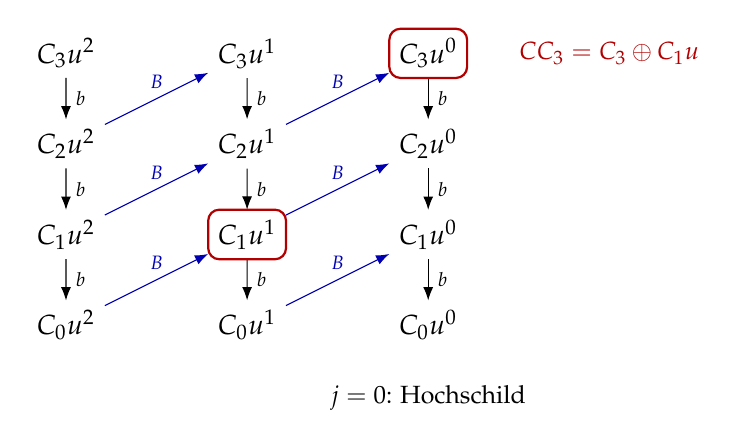
\begin{tikzpicture}[>=Latex,xscale=2.3,yscale=1.15]
 \foreach \j in {0,1,2}{
  \foreach \k in {0,1,2,3}{
    \node (c\j\k) at (-\j,\k) {\(C_{\k}u^{\j}\)};
  }
 }
 \foreach \j in {0,1,2}{
  \foreach \k in {1,2,3}{
    \pgfmathtruncatemacro{\km}{\k-1}
    \draw[->] (c\j\k) -- node[right,font=\scriptsize]{\(b\)} (c\j\km);
  }
 }
 \foreach \j in {1,2}{
  \pgfmathtruncatemacro{\jm}{\j-1}
  \foreach \k in {0,1,2}{
    \pgfmathtruncatemacro{\kp}{\k+1}
    \draw[->,blue!70!black] (c\j\k) -- node[above,font=\scriptsize]{\(B\)} (c\jm\kp);
  }
 }
 \node[font=\small] at (0,-0.8) {\(j=0\): Hochschild};
 \draw[red!70!black,thick,rounded corners] (c03.south west) rectangle (c03.north east);
 \draw[red!70!black,thick,rounded corners] (c11.south west) rectangle (c11.north east);
 \node[red!70!black,font=\small,anchor=west] at (0.45,3) {\(CC_3=C_3\oplus C_1u\)};
\end{tikzpicture}
\caption[The \((b,B)\) bicomplex]{The \((b,B)\) bicomplex. The column
\(u^j\) is a copy of the Hochschild complex shifted by \(2j\); \(b\) goes down a
column, and \(u^{-1}B\) goes one column to the right and one step up in
Hochschild degree. Total degree is Hochschild degree plus \(2j\), so
\(CC_3=C_3\oplus C_1u\) (boxed).}
\label{fig:bB}
\end{figure}

\begin{proposition}[The \(SBI\) sequence]\label{prop:SBI}
There is a long exact sequence
\[
 \cdots\to\HH_N(A)\xrightarrow{I}\HC_N(A)\xrightarrow{S}\HC_{N-2}(A)
 \xrightarrow{\pa}\HH_{N-1}(A)\to\cdots,
\]
where \(I\) is the inclusion of the column \(j=0\), \(S(\sum_jc_ju^j)=
\sum_{j\ge1}c_ju^{j-1}\), and \(\pa[\sum_jz_ju^j]=[Bz_0]\).
\end{proposition}

\begin{proof}
\(0\to C_\bullet\xrightarrow{I}CC_\bullet\xrightarrow{S}CC_{\bullet-2}\to0\) is a
short exact sequence of complexes. For the connecting map, lift a cycle
\(z=\sum z_ju^j\in CC_{N-2}\) to \(\sum_jz_ju^{j+1}\in CC_N\), and apply
\(b+u^{-1}B\). For \(i\ge1\) the coefficient of \(u^i\) is \(bz_{i-1}+Bz_i\),
which vanishes because it is the coefficient of \(u^{i-1}\) in
\((b+u^{-1}B)z=0\). The coefficient of \(u^0\) is \(Bz_0\).
\end{proof}

A \emph{mixed complex} is a complex \((C,b)\) with an operator \(B\) of degree
\(+1\) such that \(B^2=0\) and \(bB+Bb=0\). The cyclic complex and the \(SBI\)
sequence make sense for any mixed complex, and they are natural for maps
commuting with \(b\) and \(B\).

\begin{lemma}\label{lem:HHtoHC}
A map of mixed complexes that induces isomorphisms on the homology of
\(b\) induces isomorphisms on cyclic homology.
\end{lemma}

\begin{proof}
Induction on \(N\), with \(\HC_N=0\) for \(N<0\) and \(\HC_0=\HH_0\). The map of
\(SBI\) sequences and the five lemma give the step from \(N-1\) and \(N-2\) to
\(N\).
\end{proof}

\begin{theorem}[Connes \cite{Connes}]\label{thm:HCsmooth}
For a manifold \(M\) without boundary,
\[
 \HC_N(\CI(M))\cong\Om^N(M)/d\Om^{N-1}(M)\oplus H^{N-2}(M)\oplus
 H^{N-4}(M)\oplus\cdots .
\]
\end{theorem}

\begin{proof}
By Theorem~\ref{thm:connes} and Proposition~\ref{prop:Bd}, \(\chi\) is a map
of mixed complexes from \((C(\CI(M)),b,B)\) to \((\Om(M),0,d)\) that induces an
isomorphism on the homology of \(b\). By Lemma~\ref{lem:HHtoHC} it suffices
to compute the cyclic homology of \((\Om,0,d)\). Its cyclic complex is
\(\bigoplus_j\Om^{N-2j}u^j\) with differential
\(\sum_j\omega_ju^j\mapsto\sum_{j\ge1}d\omega_ju^{j-1}\). A cycle has
\(d\omega_j=0\) for \(j\ge1\) and \(\omega_0\) arbitrary, and the boundaries are
the sums with \(\omega_j\in d\Om^{N-2j-1}\). This gives the stated answer.
\end{proof}

\subsection{Periodic cyclic homology}\label{subsec:HP}
Allow all \(j\in\Z\) and infinite products:
\(CP_N(A)=\prod_{j\in\Z}C_{N-2j}(A)u^j\), with the same differential, now with
\(u^{-1}\) invertible. Its homology \(\HP_N(A)\) depends only on the parity of
\(N\). For \((\Om,0,d)\) the computation above gives
\(\HP_0=H^{\mathrm{ev}}(M)\) and \(\HP_1=H^{\mathrm{odd}}(M)\), so periodic
cyclic homology sees exactly de Rham cohomology. By the Milnor sequence
(G10) there is an exact sequence
\[
 0\to\varprojlim\nolimits^1_S\HC_{N+2j+1}(A)\to\HP_N(A)\to
 \varprojlim\nolimits_S\HC_{N+2j}(A)\to0 ,
\]
the limits being taken along \(S\). If all the maps \(S\) are surjective,
the \(\varprojlim^1\) term vanishes. We use this only in
Corollary~\ref{cor:HPP}.

\section{A primer on spectral sequences}\label{sec:ss}

\begin{whatdoes}
A spectral sequence computes the homology of a complex one ``order'' at a
time. We set up the only kind we need, explain its first pages on tiny
examples, and prove two convergence results: a general criterion
(Proposition~\ref{prop:criterion}) and the special case in which the second
page lies on one line (Proposition~\ref{prop:line}). The second is what
makes the computation of \cite{BG} work.
\end{whatdoes}

\subsection{Filtered complexes of formal sums}\label{subsec:filtered}
All our complexes have the following form. For each degree \(k\) there are
vector spaces \(C_{p,k}\), \(p\in\Z\), and
\[
 C_k=\Bigl\{c=\sum_{p\le P}c_p:\ c_p\in C_{p,k},\ P\in\Z\Bigr\},
\]
formal sums with orders bounded above (or a subspace of this, containing each
\(C_{p,k}\)). We call \(p\) the \emph{order}. The differential has the form
\[
 b=\sum_{l\ge0}b_l,\qquad b_l:C_{p,k}\to C_{p-l,k-1},
\]
so it never raises order, and \(b_l\) lowers it by exactly \(l\). The
component of order \(p\) of \(bc\) is the finite sum \(\sum_lb_lc_{p+l}\). The
subspaces \(F_pC=\{c:\ c_q=0\text{ for }q>p\}\) form an increasing
\emph{filtration} by subcomplexes. Comparing orders in \(b^2=0\) gives
\begin{equation}\label{eq:bl}
 \sum_{i+j=l}b_ib_j=0,\qquad\text{in particular}\quad b_0^2=0,\quad
 b_0b_1+b_1b_0=0 .
\end{equation}

\begin{definition}\label{def:E1E2}
The \emph{zeroth page} is \((C_{p,\bullet},b_0)\). The \emph{first page} is
\(E^1_{p,k}=H_k(C_{p,\bullet},b_0)\). By \eqref{eq:bl}, \(b_1\) maps
\(b_0\)-cycles to \(b_0\)-cycles and \(b_0\)-boundaries to \(b_0\)-boundaries, so it
induces \(d^1:E^1_{p,k}\to E^1_{p-1,k-1}\) with \((d^1)^2=0\). The \emph{second
page} is \(E^2_{p,k}=\ker d^1/\Ran d^1\) at \((p,k)\).
\end{definition}

The filtration is \emph{complete} if every series \(\sum_je_j\) with
\(e_j\in F_{p_j}C_k\), \(\sup_jp_j<\infty\) and \(p_j\to-\infty\) defines an element
of \(C_k\) (each order receives finitely many contributions), and \(b\) commutes
with such sums. For the full space of formal sums this is automatic. It is
\emph{not} automatic for subspaces, and this is the source of the
convergence issue in Remark~\ref{rem:convergence}. If \(C_{p,k}=0\) for all
\(p<0\), every series of this kind is finite, and completeness is trivial.

\begin{discussion}
Think of a cycle \(c=c_P+c_{P-1}+\cdots\) as an expansion in a small parameter,
with \(c_P\) the leading term. The equation \(bc=0\) at the top order is
\(b_0c_P=0\): the leading term is a cycle for the ``classical'' differential
\(b_0\). At the next order it reads \(b_1c_P+b_0c_{P-1}=0\): the first correction
\(b_1\) applied to \(c_P\) must be a \(b_0\)-boundary. So the leading term of a
genuine cycle defines a class in \(E^1\) killed by \(d^1\). Conversely, the
leading term of a boundary \(b(x+y)\) is \(b_1x+b_0y\), and so lies in the
image of \(d^1\). Thus \(E^2\) is a first approximation to the homology: the
leading terms of cycles modulo the leading terms of boundaries, computed to
first order.
\end{discussion}

\subsection{Three tiny examples}\label{subsec:tiny}
\begin{example}[\(d^1\) kills]\label{ex:tiny1}
Let \(C_1=\C e\) with \(e\) of order \(1\), \(C_0=\C f\) with \(f\) of order \(0\),
and \(be=f\). Then \(b=b_1\), \(b_0=0\), so \(E^1\) is spanned by \([e]\) and \([f]\),
and \(d^1[e]=[f]\). Hence \(E^2=0\), which is the homology of \(C\).
\end{example}

\begin{example}[A longer differential]\label{ex:tiny2}
Now give \(e\) order \(2\) and keep \(be=f\). Then \(b=b_2\) and
\(b_0=b_1=0\), so \(E^1=E^2\) is spanned by \([e]\) and \([f]\), but the homology
is zero. The second page is not the answer: a further differential
\(d^2:E^2_{2,1}\to E^2_{0,0}\), induced by \(b_2\), sends \([e]\) to \([f]\). In
general there are pages \(E^r\) and differentials \(d^r:E^r_{p,k}\to
E^r_{p-r,k-1}\), each the homology of the previous one (G4). The differential
\(d^r\) is computed by a \emph{zig-zag}: lift a class to \(x\) with
\(bx\in F_{p-r}\), and take the leading term of \(bx\).
\end{example}

\begin{example}[A correction term: the Weyl algebra]\label{ex:tiny3}
Filter \(A_1\) by order in \(\pa\), and Hochschild chains by total order. The
chain \(c_1=1\otimes x\otimes\pa-1\otimes\pa\otimes x\) has order \(1\). Its boundary has
order \(0\): \(bc_1=1\otimes[\pa,x]=1\otimes1\). In the language above, \(c_1\) is a
\(b_0\)-cycle, since the associated graded algebra \(\C[x,\xi]\) is commutative,
but \(b_1c_1=1\otimes1\neq0\). This is a \(b_0\)-boundary, \(1\otimes1=b_0(1\otimes1\otimes1)\),
so we correct: \(c=c_1-1\otimes1\otimes1\) is a cycle (Example~\ref{ex:weylcycle}).
The leading term \(c_1\) survives to \(E^2\), and the correction \(c_0=-1\otimes1\otimes1\)
was found by solving \(b_0c_0=-b_1c_1\).
\end{example}

The spectral sequence \emph{degenerates at \(E^2\)} if all \(d^r\), \(r\ge2\), are
zero. It \emph{converges} if \(E^\infty\), the page at which it stabilizes, is
the associated graded of \(H(C)\) for the filtration
\(F_pH=\Ran(H(F_pC)\to H(C))\), and if \(H(C)\) is recovered from its
associated graded (exhaustive, separated and complete). We need neither
the general theory nor the pages \(E^r\), \(r\ge3\): the two propositions
below are proved directly from Definition~\ref{def:E1E2}.

\subsection{The basic step and a convergence criterion}\label{subsec:criterion}

\begin{lemma}[Step (P)]\label{lem:stepP}
Let \(c\in F_pC_k\) with \(b_0c_p=0\) and \(b_1c_p+b_0c_{p-1}=0\) (for instance
\(bc\in F_{p-2}\)). If the class of \(c_p\) in \(E^2_{p,k}\) is zero, there are
\(x\in C_{p+1,k+1}\) with \(b_0x=0\) and \(y\in C_{p,k+1}\) such that
\(c-b(x+y)\in F_{p-1}C_k\).
\end{lemma}

\begin{proof}
The class \([c_p]\in E^1_{p,k}\) is a \(d^1\)-cycle, and since it is zero in
\(E^2\), it equals \(d^1[x]=[b_1x]\) for a \(b_0\)-cycle \(x\in C_{p+1,k+1}\). So
\(c_p-b_1x=b_0y\) for some \(y\in C_{p,k+1}\). The components of \(b(x+y)\) of
orders \(p+1\) and \(p\) are \(b_0x=0\) and \(b_1x+b_0y=c_p\).
\end{proof}

Say that \emph{(S) holds at \((p,k)\)} if every class in \(E^2_{p,k}\) is the
class of the leading term \(z_p\) of a cycle \(z\in F_pC_k\). Let
\(F_pH_k\subset H_k(C)\) be the classes having a representative in \(F_pC_k\).

\begin{proposition}[Convergence criterion]\label{prop:criterion}
Let the filtration be complete, and fix \(k\). Suppose (S) holds at
\((q,k+1)\) for all \(q\) and at \((p,k)\) for all \(p\). Then:
\begin{enumerate}
\item for each \(p\), \(\Theta_p[c]=[c_p]\), for cycles \(c\in F_pC_k\), is a
well-defined surjection \(F_pH_k\to E^2_{p,k}\) with kernel \(F_{p-1}H_k\);
\item \(\bigcap_pF_pH_k=0\);
\item \(H_k=\bigcup_pF_pH_k\).
\end{enumerate}
\end{proposition}

\begin{proof}
(3) holds because every chain has bounded order.

(1) \emph{Well defined.} Let \(w=be\in F_pC_k\) with \(e\in F_qC_{k+1}\). We show
\([w_p]=0\) in \(E^2_{p,k}\). If \(q\le p+1\), then \(b_0e_{p+1}=w_{p+1}=0\) and
\(w_p=b_1e_{p+1}+b_0e_p\), so \([w_p]=d^1[e_{p+1}]=0\). If \(q>p+1\), then
\(b_0e_q=w_q=0\) and \(b_1e_q+b_0e_{q-1}=w_{q-1}=0\), so \(e_q\) defines a class in
\(E^2_{q,k+1}\). By (S) there is a cycle \(z\in F_qC_{k+1}\) with the same class,
that is \(z_q-e_q=b_1x+b_0y\) with \(x\) a \(b_0\)-cycle of order \(q+1\) and \(y\) of
order \(q\). Then \(e'=e-z+b(x+y)\) lies in \(F_{q-1}\), because its components of
orders \(q+1\) and \(q\) are \(-b_0x=0\) and \(e_q-z_q+b_1x+b_0y=0\); and \(be'=be\).
Repeating, we reach \(q\le p+1\).
\emph{Surjective}: this is (S) at \((p,k)\). \emph{Kernel}: if \([c_p]=0\),
Lemma~\ref{lem:stepP} gives a homologous cycle in \(F_{p-1}\); conversely a
class in \(F_{p-1}H_k\) has a representative with \(c_p=0\).

(2) Let \(c\in F_PC_k\) be a cycle whose class lies in every \(F_pH_k\). By (1),
\(\Theta_P[c]=0\), so Lemma~\ref{lem:stepP} gives \(e_P\in F_{P+1}C_{k+1}\) with
\(c^{(1)}=c-be_P\in F_{P-1}\). Its class still lies in every \(F_pH_k\), so we
can repeat, obtaining \(e_{P-r}\in F_{P-r+1}\) with
\(c-b\sum_{s=0}^{r}e_{P-s}\in F_{P-r-1}\). By completeness \(e=\sum_se_{P-s}\)
exists and \(c-be\) lies in \(\bigcap_pF_pC_k=0\).
\end{proof}

\subsection{When the second page lies on a line}\label{subsec:line}

\begin{proposition}[Degeneration and convergence {\cite[Ch.~10]{MelroseMicro}}]
\label{prop:line}
Let the filtration be complete, and suppose there is an integer \(n\) such that
\(E^2_{p,k}=0\) whenever \(p\neq k-n\). Then every class in \(H_k(C)\) has a
representative in \(F_{k-n}C_k\), and
\[
 \Theta:H_k(C)\to E^2_{k-n,k},\qquad [c]\mapsto[c_{k-n}]\quad(c\in F_{k-n}C_k),
\]
is an isomorphism.
\end{proposition}

\begin{proof}
We verify (S). Off the line \(E^2=0\), so (S) is trivial there. Let
\(x\in C_{k-n,k}\) be a \(b_0\)-cycle with \(d^1[x]=0\). Then \(b_1x=-b_0y\) for some
\(y\in C_{k-n-1,k}\), and \(c^{(1)}=x+y\) satisfies \(bc^{(1)}\in F_{k-n-2}\).
Suppose \(c^{(r)}\in F_{k-n}C_k\) has leading term \(x\) and
\(z=bc^{(r)}\in F_{p}C_{k-1}\) with \(p=k-n-r-1\). Then \(z\) is a cycle, and
\(p\neq(k-1)-n\), so \(E^2_{p,k-1}=0\) and Lemma~\ref{lem:stepP} gives
\(x'\in C_{p+1,k}\), \(y'\in C_{p,k}\) with \(z-b(x'+y')\in F_{p-1}\). Put
\(c^{(r+1)}=c^{(r)}-x'-y'\). Since \(p+1<k-n\), its leading term is still \(x\), and
\(bc^{(r+1)}\in F_{p-1}\). The corrections have orders tending to \(-\infty\), so
by completeness \(c=\lim_rc^{(r)}\) exists; it is a cycle, because \(bc\) lies in
every \(F_p\), and its leading term is \(x\).

Now apply Proposition~\ref{prop:criterion}. Since \(E^2_{p,k}=0\) for
\(p>k-n\), part (1) gives \(F_pH_k=F_{p-1}H_k\) for \(p>k-n\), and with (3) every
class lies in \(F_{k-n}H_k\). Since \(E^2_{p,k}=0\) for \(p<k-n\), the same argument
gives \(F_{k-n-1}H_k=F_pH_k\) for all \(p<k-n\), and by (2) this is zero. So
\(\Theta=\Theta_{k-n}\) is an isomorphism \(H_k=F_{k-n}H_k\to E^2_{k-n,k}\).
\end{proof}

Figure~\ref{fig:ss} shows the mechanism. The higher differentials \(d^r\)
of Example~\ref{ex:tiny2} map \((p,k)\) to \((p-r,k-1)\). If \(E^2\) lives on the
line \(p=k-n\), the source and target can both be on the line only if
\(r=1\). So \(d^r=0\) for \(r\ge2\): the spectral sequence \emph{degenerates}. The
proposition shows, in addition, that the answer is not lost in the
infinite tail of the filtration: it \emph{converges}.

\begin{figure}[htbp]
\centering
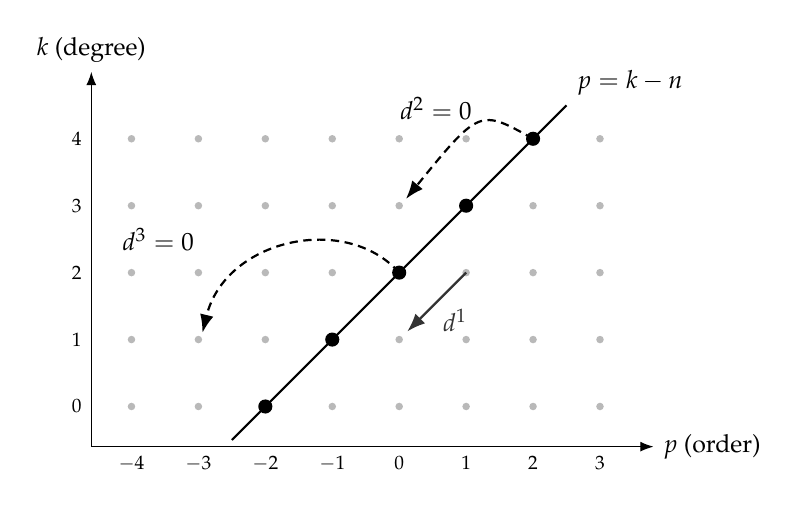
\begin{tikzpicture}[>=Latex,scale=0.85]
  \foreach \p in {-4,...,3}{
    \foreach \k in {0,...,4}{
      \fill[gray!55] (\p,\k) circle (1.6pt);
    }
  }
  \draw[->] (-4.6,-0.6) -- (3.8,-0.6) node[right] {\small \(p\) (order)};
  \draw[->] (-4.6,-0.6) -- (-4.6,5.0) node[above] {\small \(k\) (degree)};
  \foreach \p in {-4,...,3} \node[below] at (\p,-0.6) {\scriptsize \(\p\)};
  \foreach \k in {0,...,4} \node[left] at (-4.6,\k) {\scriptsize \(\k\)};
  \draw[thick] (-2.5,-0.5) -- (2.5,4.5) node[above right] {\small \(p=k-n\)};
  \foreach \k in {0,...,4} \fill (\k-2,\k) circle (3pt);
  \draw[->,thick,gray!40!black] (1,2) -- node[below right=-2pt] {\small \(d^1\)} (0.12,1.12);
  \draw[->,thick,densely dashed] (2,4) .. controls (1.2,4.45) .. (0.1,3.1);
  \node at (0.55,4.45) {\small \(d^2=0\)};
  \draw[->,thick,densely dashed] (0,2) .. controls (-0.8,2.9) and (-2.6,2.5) .. (-2.94,1.1);
  \node at (-3.6,2.5) {\small \(d^3=0\)};
\end{tikzpicture}
\caption[The order spectral sequence and its line]{The spectral sequence of the
order filtration for a symbol algebra, drawn for \(n=2\). Gray dots mark the
positions \((p,k)\) where \(E^1_{p,k}\) (homogeneous \(k\)-forms of degree \(p\)) can
be non-zero. The differential \(d^1\) moves along lines parallel to \(p=k-n\).
In BG's situation \(E^2\) lives on the line \(p=k-n\) (black dots), while
\(d^r\), \(r\ge2\), maps \((p,k)\) to \((p-r,k-1)\), off the line, so it vanishes.}
\label{fig:ss}
\end{figure}

\begin{figure}[htbp]
\centering
\begin{tikzpicture}[>=Latex,xscale=1.6,yscale=1.1]
 \draw[->] (-0.5,-0.5)--(3.6,-0.5) node[right] {\small order \(p\)};
 \draw[->] (-0.5,-0.5)--(-0.5,2.6) node[above] {\small degree \(k\)};
 \foreach \p in {0,1,2,3} \node[below,font=\scriptsize] at (\p,-0.5) {\(\p\)};
 \foreach \k in {0,1,2} \node[left,font=\scriptsize] at (-0.5,\k) {\(\k\)};
 \node[fill=white,inner sep=1pt] (x) at (3,2) {\(x\)};
 \node[fill=white,inner sep=1pt] (y) at (2,2) {\(y\)};
 \node[fill=white,inner sep=1pt] (c) at (2,1) {\(c_p\)};
 \draw[->,thick] (x) -- node[below right,font=\footnotesize]{\(b_1\)} (c);
 \draw[->,thick,blue!70!black] (y) -- node[left,font=\footnotesize]{\(b_0\)} (c);
 \node[font=\footnotesize,align=left,anchor=west] at (3.25,1.2) {\(c_p=b_1x+b_0y\)\\ \(\Rightarrow c-b(x+y)\in F_{p-1}\)};
 
\end{tikzpicture}
\caption[Step (P)]{Step (P) of Lemma~\ref{lem:stepP}, drawn for \(p=2\),
\(k=1\). If the leading term \(c_p\) of a cycle is zero in \(E^2\), it is
\(b_1x+b_0y\) with \(x\) one order higher, and subtracting the boundary
\(b(x+y)\) lowers the order of the cycle. Iterating step (P) and summing the
corrections is where completeness is used.}
\label{fig:stepP}
\end{figure}

\begin{question}
The Weyl algebra and \(\cD(\R^n)\) have orders \(\ge0\), while symbols have orders
unbounded below. Does that matter?
\end{question}
\begin{answer}
Yes, for convergence. If \(C_{p,k}=0\) for \(p<0\), every chain is a finite sum,
completeness is automatic, and Proposition~\ref{prop:line} applies to any
subcomplex of finite sums. For symbols the corrections in the proof form an
infinite series, and one must decide which infinite sums are chains. This
is the content of Section~\ref{subsec:chainmodels} and Appendix~\ref{app:mixed}.
\end{answer}

\section{Poisson manifolds and the operator \texorpdfstring{\(\delta\)}{delta}}
\label{sec:poisson}

\begin{whatdoes}
We start from the Poisson bracket that appears in the symbol of a
commutator, introduce the symplectic form, Hamiltonian vector fields and
the Poisson bivector on \(T^*\R^n\), and only then the general definitions.
We compute the Koszul--Brylinski operator \(\delta\) on \(\R^2\) by hand, and
then prove the general results: the formula for \(\delta\), Brylinski's
theorem \(\delta=\pm*^{-1}d*\), and the de Rham cohomology of homogeneous
forms.
\end{whatdoes}

\subsection{From commutators to Poisson brackets}\label{subsec:fromcomm}
\begin{lemma}\label{lem:commutator}
If \(A\in\Psi^m\) and \(B\in\Psi^{m'}\) have principal symbols \(a\), \(b\), then
\([A,B]\in\Psi^{m+m'-1}\) and \(\sigma_{m+m'-1}([A,B])=-i\{a,b\}\).
\end{lemma}

\begin{proof}
In the composition formula \eqref{eq:intro-comp} the terms with \(\alpha=0\)
cancel in \(a\#b-b\#a\). The terms with \(|\alpha|=1\) give, at top order,
\(\sum_j(\pa_{\xi_j}a\,D_{x_j}b-\pa_{\xi_j}b\,D_{x_j}a)=-i\{a,b\}\), and the rest has
lower order.
\end{proof}

The bracket is bilinear and antisymmetric, satisfies the Leibniz rule
\(\{a,bc\}=\{a,b\}c+b\{a,c\}\), and satisfies the Jacobi identity
\[
 \{a,\{b,c\}\}+\{b,\{c,a\}\}+\{c,\{a,b\}\}=0 .
\]
The Jacobi identity can be checked directly, but Lemma~\ref{lem:commutator}
gives a proof without computation. The commutator satisfies the Jacobi
identity, and \(\sigma([A,[B,C]])=(-i)^2\{a,\{b,c\}\}\). So the Jacobi identity
holds for principal symbols, that is, for all homogeneous functions on
\(\Tdot\R^n\). It is a trilinear differential identity in \(a,b,c\). The jets at a point
\((x_0,\xi_0)\), \(\xi_0\ne0\), of homogeneous functions of a \emph{fixed} degree are not
arbitrary (Euler's relation fixes the radial derivatives), but finite sums of
homogeneous functions of different integer degrees have arbitrary jets of any
finite order: restricted to a small conic neighbourhood, \(|\xi|^j\) for
\(j=0,1,\dots,J\) times functions on the sphere bundle already gives every
polynomial of degree \(\le J\) in \(|\xi|-|\xi_0|\). By multilinearity the identity holds
for such sums, hence for all smooth functions.

\subsection{The symplectic form and Hamiltonian vector fields on \texorpdfstring{\(T^*\R^n\)}{T*Rn}}
\label{subsec:symplecticRn}
On \(T^*\R^n\) with coordinates \((x,\xi)\) we have the symplectic form
\(\omega=\sum_jd\xi_j\wedge dx_j\) and, for a function \(f\), the
\emph{Hamiltonian vector field} \(H_f\), defined by \(\iota_{H_f}\omega=-df\). In
coordinates \(H_f=\sum_j(\pa_{\xi_j}f\,\pa_{x_j}-\pa_{x_j}f\,\pa_{\xi_j})\), and
\(\{f,g\}=H_fg=\omega(H_f,H_g)\). The Hamiltonian flow of the principal symbol of
an operator is the classical motion that the operator quantizes; for
instance on \(\R^2\), \(f=\frac12(x^2+\xi^2)\) gives \(H_f=\xi\pa_x-x\pa_\xi\), a
rotation.

The \emph{Poisson bivector} \(\pi\) is the antisymmetric form on covectors
with \(\pi(df,dg)=\{f,g\}\). In coordinates
\(\pi=\sum_j\pa_{\xi_j}\wedge\pa_{x_j}\) and
\(\pi(\theta,\eta)=\sum_j(\theta(\pa_{\xi_j})\eta(\pa_{x_j})-\theta(\pa_{x_j})
\eta(\pa_{\xi_j}))\). Let \(\pi^\sharp\theta\) be the vector with
\(\eta(\pi^\sharp\theta)=\pi(\theta,\eta)\). Then \(\pi^\sharp(df)=H_f\), and
\(\iota_{\pi^\sharp\theta}\omega=-\theta\) for every covector \(\theta\): \(\pi\) is the
inverse of \(\omega\), up to sign.

The \emph{radial vector field} \(R=\sum_j\xi_j\pa_{\xi_j}\) generates the dilations
\(\rho_t\). Since \(\rho_t^*\omega=t\omega\), we have \(\Lie_R\omega=\omega\): the
symplectic form is homogeneous of degree \(1\). Moreover \(\iota_R\omega=
\alpha=\sum\xi_j\,dx_j\), so by Cartan's formula \(\Lie_R\omega=d\iota_R\omega=d\alpha=\omega\).

\subsection{Poisson and symplectic manifolds}\label{subsec:poissondef}
\begin{definition}[{\cite[\S1]{BG}}]
A \emph{Poisson bracket} on a commutative algebra \(A\) is a bilinear map
\(\{\cdot,\cdot\}\) making \(A\) a Lie algebra and satisfying the Leibniz rule
\(\{f,gh\}=g\{f,h\}+h\{f,g\}\). A \emph{Poisson manifold} is a manifold with a
Poisson bracket on \(\CI\); the bracket is then \(\{f,g\}=\pi(df,dg)\) for a
bivector field \(\pi\), by the Leibniz rule.
\end{definition}

A \emph{symplectic manifold} \((X,\omega)\) is a manifold of dimension \(2n\)
with a closed non-degenerate \(2\)-form. It is Poisson: define \(H_f\) by
\(\iota_{H_f}\omega=-df\) and \(\{f,g\}=H_fg\). By Darboux's theorem (G6), near
every point there are coordinates \((x,\xi)\) with \(\omega=\sum d\xi_j\wedge dx_j\),
so all the formulas of Section~\ref{subsec:symplecticRn} hold locally. On a
cotangent bundle \(T^*M\) the canonical coordinates are Darboux coordinates,
and no theorem is needed. BG write \(H_gf=\{f,g\}\), which is our \(-H_g\);
see Remark~\ref{rem:hamsign}.

\subsection{The operator \texorpdfstring{\(\delta\)}{delta} on the plane}
\label{subsec:poissonR2}
On \(\R^2\) with \(\omega=d\xi\wedge dx\), let \(\iota_\pi\) be contraction with the
bivector: \(\iota_\pi=0\) on functions and \(1\)-forms, and
\(\iota_\pi(h\,d\xi\wedge dx)=h\). Put \(\delta=\iota_\pi d-d\iota_\pi\). Then
\begin{align*}
 \delta f&=\iota_\pi(df)=0,\\
 \delta(f\,dg)&=\iota_\pi(df\wedge dg)=\iota_\pi\bigl((f_\xi g_x-f_xg_\xi)\,d\xi\wedge dx\bigr)=\{f,g\},\\
 \delta(h\,\omega)&=-d\iota_\pi(h\,\omega)=-dh .
\end{align*}
So \(\delta\) lowers degree by one. It is a differential:
\(\delta^2(h\omega)=-\delta(dh)=-\{1,h\}=0\). Its homology on smooth forms is
easy to compute. On \(2\)-forms, \(\ker\delta=\C\,\omega\). On \(1\)-forms,
\(\ker\delta\) is the space of closed forms, since \(\delta\theta=\iota_\pi d\theta\), and the
image of \(\delta\) is the space of exact forms; the quotient is
\(H^1(\R^2)=0\). On functions, every \(h\) is \(\{\xi,G\}=\pa_xG\) with
\(G=\int_0^xh\). Hence
\[
 H_k(\Om^\bullet(\R^2),\delta)\cong H^{2-k}(\R^2)=\begin{cases}\C,&k=2,\\0,&k\ne2.\end{cases}
\]
The duality \(k\leftrightarrow2-k\) is explained by a star operator. Define
\(*1=\omega\), \(*\omega=1\), and \(*=\mathrm{id}\) on \(1\)-forms. Then
\(*d*(f\,dg)=*(df\wedge dg)=\{f,g\}\) and \(-*d*(h\omega)=-dh\), so
\[
 \delta=(-1)^{k-1}\,*d*\qquad\text{on \(k\)-forms on \(\R^2\)}.
\]
This is Brylinski's theorem in its smallest case. The rest of this section
proves it in general.

\subsection{The Koszul--Brylinski operator}\label{subsec:delta}
Let \((X,\omega)\) be symplectic of dimension \(2n\), with Poisson bivector \(\pi\).
Define \(\iota_\pi:\Om^k\to\Om^{k-2}\) by
\[
 \iota_\pi(\theta_1\wedge\dots\wedge\theta_k)=\sum_{j<l}(-1)^{j+l+1}\pi(\theta_j,\theta_l)\,
 \theta_1\wedge\dots\widehat{\theta_j}\dots\widehat{\theta_l}\dots\wedge\theta_k .
\]
In Darboux coordinates \(\iota_\pi=\sum_j\iota_{\pa_{x_j}}\iota_{\pa_{\xi_j}}\). Following
Koszul \cite{Koszul} and Brylinski \cite{Brylinski}, set
\[
 \delta=[\iota_\pi,d]=\iota_\pi d-d\iota_\pi:\Om^k(X)\to\Om^{k-1}(X).
\]

\begin{lemma}\label{lem:deltaformula}
For functions \(a_0,\dots,a_k\),
\begin{multline*}
 \delta(a_0\,da_1\wedge\dots\wedge da_k)=\sum_{j=1}^k(-1)^{j+1}\{a_0,a_j\}\,
 da_1\wedge\dots\widehat{da_j}\dots\wedge da_k\\
 +\sum_{1\le j<l\le k}(-1)^{j+l}a_0\,d\{a_j,a_l\}\wedge da_1\wedge\dots
 \widehat{da_j}\dots\widehat{da_l}\dots\wedge da_k .
\end{multline*}
Moreover, if \(\beta\) has constant coefficients in Darboux coordinates, then
\(\delta(f\beta)=\iota_{H_f}\beta\). Finally, for every \(1\)-form \(\theta\),
\begin{equation}\label{eq:iotapieps}
 [\iota_\pi,\eps(\theta)]=\iota_{\pi^\sharp\theta},
\end{equation}
where \(\eps(\theta)\) is exterior multiplication by \(\theta\).
\end{lemma}

\begin{proof}
Write \(D_{jl}\) for \(da_1\wedge\dots\wedge da_k\) with \(da_j\) and \(da_l\) omitted,
and \(D_{0l}\) when only \(da_l\) is omitted. Applying \(\iota_\pi\) to
\(da_0\wedge da_1\wedge\dots\wedge da_k\), the pairs \((0,l)\) give
\(\sum_l(-1)^{l+1}\{a_0,a_l\}D_{0l}\), and the pairs \(1\le j<l\) give
\(\sum(-1)^{j+l+1}\{a_j,a_l\}\,da_0\wedge D_{jl}\). On the other hand
\(d\iota_\pi(a_0\,da_1\wedge\dots\wedge da_k)=\sum_{j<l}(-1)^{j+l+1}
(\{a_j,a_l\}\,da_0+a_0\,d\{a_j,a_l\})\wedge D_{jl}\). Subtracting gives the
formula. For \eqref{eq:iotapieps}, for vector fields \(V\), \(W\) one has
\(\iota_V\iota_W\eps(\theta)-\eps(\theta)\iota_V\iota_W=\theta(W)\iota_V-\theta(V)\iota_W\), from
\(\iota_W\eps(\theta)+\eps(\theta)\iota_W=\theta(W)\). With \(V=\pa_{x_j}\), \(W=\pa_{\xi_j}\),
summed over \(j\), the right side is \(\iota_{\pi^\sharp\theta}\). For the middle
statement, \(d\beta=0\) and \(d\iota_\pi\beta=0\), so \(\delta(f\beta)=\iota_\pi(df\wedge\beta)-
df\wedge\iota_\pi\beta=[\iota_\pi,\eps(df)]\beta=\iota_{H_f}\beta\).
\end{proof}

\begin{correction}[The sign in BG's formula for \(\delta\)]\label{corr:delta}
In \cite[\S1, Theorem~(2)]{BG}, and again on forms in \cite[\S2]{BG}, the
second sum carries the sign \((-1)^{i+j+1}\). It should be \((-1)^{i+j}\), as in
Lemma~\ref{lem:deltaformula}. With BG's sign the operator is not well defined
on forms. Take \(k=2\) and compare \(\delta(1\cdot d(bc)\wedge dg)\) with
\(\delta(b\,dc\wedge dg+c\,db\wedge dg)\), which must agree since
\(d(bc)=b\,dc+c\,db\). With the correct sign both equal
\(-d(b\{c,g\})-d(c\{b,g\})\). With BG's sign the first is
\(+d(b\{c,g\}+c\{b,g\})\), while the second is
\(-\{b,g\}\,dc-\{c,g\}\,db+b\,d\{c,g\}+c\,d\{b,g\}\), and these differ by
\(2(\{b,g\}\,dc+\{c,g\}\,db)\). We also checked Lemma~\ref{lem:deltaformula}
symbolically against \(\iota_\pi d-d\iota_\pi\) on \(\R^4\) for \(k=2,3\). The same
calculation shows that the upper limit of the sums in \cite[\S2]{BG} should
be \(m\), not \(n\). Since the correct formula is also what the Hochschild
computation produces (Theorem~\ref{thm:d1}), the error is a misprint.
\end{correction}

\subsection{The symplectic star operator}\label{subsec:star}
Fix a point and let \(V\) be the tangent space there. On \(\Lambda^kV^*\) define the
bilinear form
\[
 \Lambda(\theta_1\wedge\dots\wedge\theta_k,\eta_1\wedge\dots\wedge\eta_k)=
 \det\bigl(\pi(\theta_i,\eta_j)\bigr)_{i,j=1}^k ,
\]
and \(\Lambda(1,1)=1\). It is non-degenerate, because
\(\Lambda(\alpha,\beta)=\pm\langle\alpha,\Lambda^k\pi^\sharp\beta\rangle\) and
\(\pi^\sharp\) is invertible.

\begin{definition}[Brylinski \cite{Brylinski}]
The \emph{symplectic star operator} \(*:\Lambda^kV^*\to\Lambda^{2n-k}V^*\) is
defined by
\[
 \alpha\wedge*\beta=\Lambda(\alpha,\beta)\,\vol\qquad\text{for all }\alpha\in\Lambda^kV^*,
 \qquad\vol=\frac{\omega^n}{n!}.
\]
\end{definition}

The wedge pairing \(\Lambda^k\times\Lambda^{2n-k}\to\Lambda^{2n}\) is non-degenerate, so \(*\) is
well defined and an isomorphism. Applied pointwise it gives isomorphisms
\(*:\Om^k(X)\to\Om^{2n-k}(X)\). In Darboux coordinates \(*\) maps
constant-coefficient forms to constant-coefficient forms. For example
\(*1=\vol\), and on \(\R^2\) we recover the operator of
Section~\ref{subsec:poissonR2}. This is the analogue of the Riemannian Hodge
star of \cite[\S``Formal adjoints and the Hodge star'']{LoyaAS}, with the
metric replaced by \(\pi\).

\begin{lemma}\label{lem:starlemma}
For \(\theta\in V^*\), \(\beta\in\Lambda^kV^*\) and \(\gamma\in\Lambda^jV^*\),
\[
 *^{-1}(\theta\wedge*\beta)=(-1)^{k-1}\iota_{\pi^\sharp\theta}\beta,\qquad
 *(\theta\wedge\gamma)=(-1)^{j+1}\iota_{\pi^\sharp\theta}(*\gamma).
\]
Consequently \(*(f_0\,df_1\wedge\dots\wedge df_m)=(-1)^{m(m+1)/2}f_0\,
\iota_{H_{f_1}}\cdots\iota_{H_{f_m}}\vol\).
\end{lemma}

\begin{proof}
Expanding the determinant along the first row,
\(\Lambda(\theta\wedge\alpha,\beta)=\Lambda(\alpha,\iota_{\pi^\sharp\theta}\beta)\), since
\(\iota_v(\eta_1\wedge\dots\wedge\eta_k)=\sum_j(-1)^{j+1}\eta_j(v)\,\eta_1\wedge\dots
\widehat{\eta_j}\dots\wedge\eta_k\) and \(\eta_j(\pi^\sharp\theta)=\pi(\theta,\eta_j)\). Let
\(\mu=*^{-1}(\theta\wedge*\beta)\). For all \(\alpha\in\Lambda^{k-1}V^*\),
\[
 \Lambda(\alpha,\mu)\vol=\alpha\wedge\theta\wedge*\beta=(-1)^{k-1}\theta\wedge\alpha\wedge*\beta
 =(-1)^{k-1}\Lambda(\alpha,\iota_{\pi^\sharp\theta}\beta)\vol .
\]
For the second identity expand along the first column instead:
\(\Lambda(\alpha,\theta\wedge\gamma)=-\Lambda(\iota_{\pi^\sharp\theta}\alpha,\gamma)\) for
\(\alpha\in\Lambda^{j+1}\), because \(\pi(\alpha_i,\theta)=-\pi(\theta,\alpha_i)\). So
\(\alpha\wedge*(\theta\wedge\gamma)=-\iota_v\alpha\wedge*\gamma\) with \(v=\pi^\sharp\theta\). Since
\(\alpha\wedge*\gamma\) has degree \(2n+1\), it vanishes, and
\(0=\iota_v(\alpha\wedge*\gamma)=\iota_v\alpha\wedge*\gamma+(-1)^{j+1}\alpha\wedge\iota_v*\gamma\).
Hence \(\alpha\wedge*(\theta\wedge\gamma)=(-1)^{j+1}\alpha\wedge\iota_v*\gamma\) for all
\(\alpha\). The last formula follows by induction from \(*1=\vol\) and
\(\pi^\sharp df=H_f\); the signs multiply to \((-1)^{1+2+\dots+m}\).
\end{proof}

\begin{theorem}[Brylinski \cite{Brylinski}]\label{thm:brylinski}
On \(k\)-forms, \(\delta=(-1)^{k-1}*^{-1}d*\). In particular \(\delta^2=0\).
\end{theorem}

\begin{proof}
Both sides are first-order differential operators, so it suffices to
compare them on \(f\beta\) with \(\beta\) of constant coefficients in Darboux
coordinates. Then \(*\beta\) has constant coefficients and
\(d(f*\beta)=df\wedge*\beta\). By Lemma~\ref{lem:starlemma},
\(*^{-1}d*(f\beta)=(-1)^{k-1}\iota_{H_f}\beta\), which is \((-1)^{k-1}\delta(f\beta)\) by
Lemma~\ref{lem:deltaformula}. Finally
\(\delta^2=\pm*^{-1}d**^{-1}d*=\pm*^{-1}d^2*=0\).
\end{proof}

\begin{figure}[htbp]
\centering
\begin{tikzcd}[column sep=4.2em,row sep=3em]
 \Om^{k+1}_{(p+1)} \arrow[r,"*","\cong"'] \arrow[d,"\delta"'] &
 \Om^{2n-k-1}_{(c)} \arrow[d,"\pm d"] \\
 \Om^{k}_{(p)} \arrow[r,"*","\cong"'] \arrow[d,"\delta"'] &
 \Om^{2n-k}_{(c)} \arrow[d,"\pm d"] \\
 \Om^{k-1}_{(p-1)} \arrow[r,"*","\cong"'] & \Om^{2n-k+1}_{(c)}
\end{tikzcd}
\caption[The \(\delta\)/\(d\) duality]{Brylinski's duality on a conic
symplectic manifold. The star operator carries \(k\)-forms homogeneous of degree
\(p\) to \((2n-k)\)-forms homogeneous of degree \(c=p+n-k\)
(Proposition~\ref{prop:starhom}), and it intertwines \(\delta\) with \(\pm d\). The
homogeneity \(c\) is the same in the whole right column: \(\delta\) lowers both the
form degree and the homogeneity by one, so \(c\) is constant along the
diagonals \(p-k=\mathrm{const}\) of Figure~\ref{fig:ss}.}
\label{fig:duality}
\end{figure}

\subsection{The \texorpdfstring{\(\mathfrak{sl}(2)\)}{sl(2)} structure and BG's star}
\label{subsec:sl2}
Let \(L=\eps(\omega)\) and \(\Lambda_\pi=\iota_\pi\), acting on \(\Lambda^\bullet V^*\).

\begin{lemma}\label{lem:sl2}
\([\iota_\pi,\eps(\omega)]=n-k\) on \(\Lambda^kV^*\).
\end{lemma}

\begin{proof}
\(\iota_\pi\) is even, so \([\iota_\pi,\eps(d\xi_j)\eps(dx_j)]=
[\iota_\pi,\eps(d\xi_j)]\eps(dx_j)+\eps(d\xi_j)[\iota_\pi,\eps(dx_j)]\). By
\eqref{eq:iotapieps} with \(\pi^\sharp(d\xi_j)=H_{\xi_j}=\pa_{x_j}\) and
\(\pi^\sharp(dx_j)=H_{x_j}=-\pa_{\xi_j}\), this is
\(\iota_{\pa_{x_j}}\eps(dx_j)-\eps(d\xi_j)\iota_{\pa_{\xi_j}}=1-\eps(dx_j)\iota_{\pa_{x_j}}
-\eps(d\xi_j)\iota_{\pa_{\xi_j}}\). Summing over \(j\) gives \(n\) minus the degree
operator.
\end{proof}

So \(L\), \(\Lambda_\pi\) and \(n-k\) span a copy of \(\mathfrak{sl}(2)\), exactly as the
Lefschetz operator, its adjoint and the degree do for a Kähler manifold.
BG define their star as \(*_{\mathrm{BG}}=\exp\bigl(\tfrac{\pi i}2(L+L^*)\bigr)\),
where \(L^*\) is the symplectic adjoint of \(L\) (a multiple of \(\Lambda_\pi\) with
\([L,L^*]=n-k\)).

\begin{correction}[The \(\mathfrak{sl}(2)\) computation]\label{corr:sl2}
BG deduce \(*_{\mathrm{BG}}^2=1\) from the identity
\[
 \exp\Bigl(\pi i\begin{pmatrix}0&1\\1&0\end{pmatrix}\Bigr)=
 \begin{pmatrix}1&0\\0&1\end{pmatrix}.
\]
In fact, for \(J=\bigl(\begin{smallmatrix}0&1\\1&0\end{smallmatrix}\bigr)\) we have \(J^2=1\) and
\(\exp(\pi iJ)=\cos\pi+i\sin\pi\,J=-1\). Worse, BG's data are not consistent with
their matrix model. They match \(\eps(\omega)\) with \(T_+\) and \(n-k\) with
\(T_0=\mathrm{diag}(1,-1)\); but \([T_0,T_+]=2T_+\), while \([n-k,\eps(\omega)]=-2\eps(\omega)\), since
\(\eps(\omega)\) raises \(k\). With our \(L^*=-\iota_\pi\) (so that \([L,L^*]=n-k\) by
Lemma~\ref{lem:sl2}), take \(n=1\) and the span of \(1\) and \(\omega\): \(L1=\omega\),
\(L^*\omega=-\iota_\pi\omega=-1\), so \(X=L+L^*\) satisfies \(X^2=-1\) there. Then
\[
 *_{\mathrm{BG}}1=\exp\bigl(\tfrac{\pi}2iX\bigr)1=\cosh\tfrac\pi2+i\sinh\tfrac\pi2\,\omega ,
\]
and \(*_{\mathrm{BG}}\) is not of finite order. (The value \(*_{\mathrm{BG}}1=i\omega\), \(*_{\mathrm{BG}}^2=-1\)
holds only in BG's matrix model.) The same issue appears in the proof of their
Proposition~(1): the series \(\sum_j\frac{(ti)^j}{j!}\ad(L+L^*)^j\) gives hyperbolic
functions of \(t\), not \(\cos t\) and \(\sin t\). The consistent fix is to drop the factor
\(i\): \(*'=\exp(\frac\pi2(L+L^*))\). Then \(*'1=\omega\), \(*'\omega=-1\), and in general
\(*'^2=\exp(\pi(L+L^*))=(-1)^{d-1}\) on an irreducible component of dimension \(d\),
since \(L+L^*\) acts there as a rotation generator with eigenvalues
\(i(d-1),i(d-3),\dots\). None of this affects the conclusions, since only
the fact that \(*\) is invertible and intertwines \(\delta\) with \(d\) up to
non-zero constants is used. We work with Brylinski's operator of
Section~\ref{subsec:star}, for which everything is proved above. (For it one
also has \(*^2=1\) \cite{Brylinski}; we checked this symbolically for \(n\le2\) and
do not use it.)
\end{correction}

\subsection{Homogeneous forms and their de Rham cohomology}\label{subsec:homdR}
Now let \(X=\Tdot M\) with its dilations and radial field \(R\). Choose a positive
function \(r\) on \(\Tdot M\), homogeneous of degree \(1\) (for instance \(|\xi|\) for a
Riemannian metric). Then \(\Tdot M\cong S^*M\times(0,\infty)\), \((x,\xi)\mapsto
((x,[\xi]),r)\), where we identify \(S^*M\) with \(\{r=1\}\).

\begin{lemma}\label{lem:Sorient}
\(\iota_R\vol\) restricts to a nowhere-vanishing form on \(S^*M\). So \(S^*M\) is
orientable, and we orient it by \(\iota_R\vol\).
\end{lemma}

\begin{proof}
\(\vol\) is nowhere zero and \(R\) is transverse to \(\{r=1\}\), since \(Rr=r\).
\end{proof}

\begin{proposition}\label{prop:starhom}
\(*\) maps \(\Om^k_{(p)}\) onto \(\Om^{2n-k}_{(p+n-k)}\).
\end{proposition}

\begin{proof}
\(\{a,b\}\) is homogeneous of degree \(p+q-1\) if \(a\), \(b\) have degrees \(p\), \(q\), so
\(\Lambda(\alpha,\beta)\) is homogeneous of degree \(p+q-k\) for
\(\alpha\in\Om^k_{(p)}\), \(\beta\in\Om^k_{(q)}\), and \(\vol\) has degree \(n\). Hence
\(\alpha\wedge\rho_t^*(*\beta)=\rho_t^*(t^{-p}\alpha\wedge*\beta)=t^{q+n-k}\alpha\wedge*\beta\). The values
of the forms \(\alpha\in\Om^k_{(p)}\) span \(\Lambda^k\) at each point, so
\(\rho_t^*(*\beta)=t^{q+n-k}*\beta\). The same argument applies to \(*^{-1}\).
\end{proof}

\begin{proposition}[Homogeneous de Rham cohomology]\label{prop:homdR}
Let \(\Om^\bullet_{(c)}\) be the complex of forms on \(\Tdot M\) homogeneous of degree
\(c\in\Z\), with \(d\).
\begin{enumerate}
\item If \(c\ne0\), the complex is acyclic: a closed \(\theta\) equals
\(d(\iota_R\theta/c)\).
\item Every \(\theta\in\Om^j_{(0)}\) can be written uniquely as
\(\theta=\theta'+\theta''\wedge dr/r\), with \(\theta'\), \(\theta''\) pulled back from \(S^*M\). This
identifies \((\Om^\bullet_{(0)},d)\) with the de Rham complex of \(S^*M\times S^1\),
\(S^1=(0,\infty)/e^{\Z}\), and
\[
 H^j(\Om^\bullet_{(0)},d)\cong H^j(S^*M)\oplus H^{j-1}(S^*M)\cong H^j(S^*M\times S^1).
\]
\item The same holds for forms that are polynomial in the fibres of
\(T^*M\), with the difference that the polynomial forms of degree \(0\) are the
forms on \(M\); their cohomology is \(H^j(M)\).
\end{enumerate}
\end{proposition}

\begin{proof}
(1) \(\iota_R\) commutes with \(\rho_t\), so it preserves homogeneity, and
\(\Lie_R=c\) on \(\Om_{(c)}\). By Cartan's formula \(d\iota_R+\iota_Rd=\Lie_R\), a closed
\(\theta\) equals \(d(\iota_R\theta)/c\).

(2) Since \(\rho_t^*(dr/r)=dr/r\), a form is homogeneous of degree \(0\) exactly
when \(\theta'\) and \(\theta''\) are independent of \(r\), that is, pulled back from
\(S^*M\). Then \(d(\theta'+\theta''\wedge dr/r)=d\theta'+d\theta''\wedge dr/r\). On
\(S^*M\times S^1\), with \(s=\log r\bmod\Z\) the coordinate on the circle,
\(dr/r=ds\), and a form on \(S^*M\times S^1\) that is invariant under rotation of
the circle is \(\theta'+\theta''\wedge ds\). The de Rham cohomology of
\(S^*M\times S^1\) is computed by invariant forms (average over the circle), and
the Künneth formula gives the last isomorphism.

(3) \(\iota_R\) preserves polynomial forms, so (1) applies. A polynomial form
of degree \(0\) has no \(d\xi\) (which has degree \(1\)) and coefficients of degree
\(0\) in \(\xi\), so it is a form on \(M\).
\end{proof}

The splitting in (2) depends on \(r\). Replacing \(r\) by \(ar\), with \(a>0\)
homogeneous of degree \(0\), changes \(\theta'\) by \(\theta''\wedge d\log a\), which does not
change the class of \(\theta''\).

\begin{question}
Why does the answer involve \(S^*M\times S^1\) rather than \(\Tdot M\), which is
homotopy equivalent to \(S^*M\)?
\end{question}
\begin{answer}
On all smooth forms, \(dr/r=d\log r\) is exact. Among \emph{homogeneous} forms
it is closed but not exact, because \(\log r\) is not homogeneous. The
symbol algebra only contains homogeneous functions, so it sees the extra
class \(dr/r\). Geometrically, dividing \((0,\infty)\) by the dilation
\(r\mapsto er\) turns the half-line into a circle, and \(dr/r\) becomes the
angular form.
\end{answer}

\section{Star products and the symbol algebra}\label{sec:star}

\begin{whatdoes}
The composition formula for symbols is a ``star product'': a deformation of
the pointwise product in which the order of a symbol plays the role of
Planck's constant. We make this precise, work out the Moyal product on
\(\R^2\), define formal deformations and BG's quantum algebras, quote the
theorem of de Wilde and Lecomte, and set up the symbol algebra \(\cP\) with its
two chain models.
\end{whatdoes}

\subsection{The composition formula is a star product}\label{subsec:compstar}
On \(\R^n\), write the composition formula \eqref{eq:intro-comp} by
homogeneity:
\[
 a\#b=\sum_{l\ge0}P_l(a,b),\qquad
 P_l(a,b)=\sum_{|\alpha|=l}\frac1{\alpha!}\,\pa_\xi^\alpha a\,D_x^\alpha b .
\]
Each \(P_l\) is a \emph{bidifferential operator}, a finite sum of products of
derivatives of \(a\) and of \(b\). If \(a\) and \(b\) are homogeneous of degrees \(p\)
and \(q\), then \(P_l(a,b)\) is homogeneous of degree \(p+q-l\). Moreover
\(P_0(a,b)=ab\) and, by Lemma~\ref{lem:commutator},
\(P_1(a,b)-P_1(b,a)=-i\{a,b\}\).

Introduce a parameter \(\hb>0\) and rescale: for a formal sum \(a=\sum_ja_j\) put
\(L_\hb a=\sum_j\hb^ja_j\), and \(a\#_\hb b=L_\hb^{-1}(L_\hb a\#L_\hb b)\). Since
\(P_l(\hb^pa_p,\hb^qb_q)=\hb^{p+q}P_l(a_p,b_q)\) has degree \(p+q-l\),
\[
 a\#_\hb b=\sum_{l\ge0}\hb^lP_l(a,b)=ab-\frac{i\hb}{2}\{a,b\}+\hb\,S(a,b)+O(\hb^2),
\]
where \(S\) is the symmetric part of \(P_1\). All these products are isomorphic, and
at \(\hb=0\) we recover the commutative product. This is the
\emph{semiclassical} picture of \cite{BG}: symbols are a deformation of the
algebra of functions on \(\Tdot M\) in the direction of the Poisson bracket, and
lowering the order by one corresponds to one power of \(\hb\). In particular
\(\hb D_x\) has symbol \(\hb\xi\), and \([x,\hb D_x]=i\hb\).

\subsection{The Moyal product}\label{subsec:moyal}
The left quantization is not symmetric in \(a\) and \(b\). The Weyl quantization is,
and its composition law is the Moyal product. On \(\R^{2n}\) let
\(\Pi=\sum_j(\pa_{\xi_j}\otimes\pa_{x_j}-\pa_{x_j}\otimes\pa_{\xi_j})\), acting on
\(a\otimes b\), so that \(m\circ\Pi(a\otimes b)=\{a,b\}\) with \(m(a\otimes b)=ab\). Define
\[
 a\star b=m\circ\exp\Bigl(\frac{\hb}{2i}\Pi\Bigr)(a\otimes b)=
 \sum_{l\ge0}\frac1{l!}\Bigl(\frac{\hb}{2i}\Bigr)^lm\circ\Pi^l(a\otimes b).
\]
For smooth \(a,b\) this is a formal power series in \(\hb\); for polynomials it is a
finite sum and we may set \(\hb=1\).

\begin{proposition}\label{prop:moyal}
The Moyal product is associative, \(a\star b-b\star a=-i\hb\{a,b\}+O(\hb^3)\), and
the term of order \(\hb^l\) is \((-1)^l\) times its transpose.
\end{proposition}

\begin{proof}
On \(a\otimes b\otimes c\) let \(\Pi_{12}\), \(\Pi_{13}\), \(\Pi_{23}\) act on the indicated factors;
they commute, since they have constant coefficients. A derivative of a product
\(fg\) is \((\pa\otimes1+1\otimes\pa)\) applied to \(f\otimes g\), so
\begin{align*}
 (a\star b)\star c&=m_3\exp\Bigl(\tfrac{\hb}{2i}(\Pi_{13}+\Pi_{23})\Bigr)
 \exp\Bigl(\tfrac{\hb}{2i}\Pi_{12}\Bigr)(a\otimes b\otimes c)\\
 &=m_3\exp\Bigl(\tfrac{\hb}{2i}(\Pi_{12}+\Pi_{13}+\Pi_{23})\Bigr)(a\otimes b\otimes c),
\end{align*}
and \(a\star(b\star c)\) gives the same expression. Transposing \(a\otimes b\) changes
\(\Pi\) into \(-\Pi\), which gives the last two statements.
\end{proof}

\begin{example}[Moyal on \(\R^2\)]\label{ex:moyalR2}
On \(\R^2\), \(\{x,\xi\}=-1\), so
\(x\star\xi=x\xi+\frac{i\hb}2\), \(\xi\star x=x\xi-\frac{i\hb}2\), and
\(\xi\star x-x\star\xi=-i\hb\). Also \(x\star x=x^2\), \(\xi\star\xi=\xi^2\), and
\(x\star(x\xi)=x^2\xi+\frac{i\hb}2x\). With \(\hb=1\), the map sending \(x\) to
multiplication by \(x\) and \(\xi\) to \(D_x=-i\pa_x\) is an isomorphism from the
polynomials with the Moyal product onto the Weyl algebra \(A_1\) (the Weyl
quantization), since \([D_x,x]=-i\). For comparison, the left-quantized product
gives \(x\#\xi=x\xi\) and \(\xi\#x=x\xi-i\).
\end{example}

\subsection{Formal deformations and quantum algebras}\label{subsec:quantum}
Let \(A\) be a commutative algebra, for instance \(\CI(X)\). Let
\(K=\C\Lser{\hb}\) be the field of formal Laurent series (finitely many negative
powers), and \(A\Lser{\hb}\) the Laurent series with coefficients in \(A\).

\begin{definition}\label{def:deformation}
A \emph{formal deformation} of \(A\) is a \(K\)-bilinear associative product on
\(A\Lser{\hb}\) of the form
\[
 a\star b=\sum_{l\ge0}\hb^lP_l(a,b)\qquad(a,b\in A),\qquad P_0(a,b)=ab ,
\]
extended \(\hb\)-linearly. It is \emph{local} if \(A=\CI(X)\) and the \(P_l\) are
bidifferential operators. A \emph{quantum algebra} in the sense of
\cite[\S1]{BG} is a formal deformation of a Poisson algebra with
\(P_1(a,b)=\{a,b\}/2i\) and \(P_l(a,b)=(-1)^lP_l(b,a)\), \(P_l(1,a)=0\).
\end{definition}

\begin{lemma}\label{lem:deformpoisson}
For a formal deformation, \(\{a,b\}_\star=i(P_1(a,b)-P_1(b,a))\) is a Poisson bracket
on \(A\).
\end{lemma}

\begin{proof}
\(a\star b-b\star a=-i\hb\{a,b\}_\star+O(\hb^2)\). The commutator is a derivation
of \(\star\) in each argument, and its leading term is a derivation of the
commutative product: compare orders \(\hb\) in \([a,b\star c]=[a,b]\star
c+b\star[a,c]\). The Jacobi identity for commutators, at order \(\hb^2\), gives
the Jacobi identity for \(\{\cdot,\cdot\}_\star\).
\end{proof}

With our conventions \(\{a,b\}_\star\) is the Poisson bracket of
Section~\ref{subsec:fromcomm} for both the Moyal and the left-quantized
products. The Moyal product on \(\R^{2n}\) is a quantum algebra in the sense
of BG, by Proposition~\ref{prop:moyal}; the left-quantized product is not.

\begin{bgremark}[Quantum algebras]\label{rem:parity}
(1) BG do not say which quantization they use for \(\cP\); their formula
\(a\star b\sim ab+\{a,b\}/2i+\cdots\) in \S4 is of symmetric (Weyl) type. The parity
condition \(P_l(a,b)=(-1)^lP_l(b,a)\) of \cite[\S1]{BG} holds for such products, but not,
for instance, for the left-quantized product of Section~\ref{subsec:symbolstar},
where \(P_1(a,b)=-i\sum\pa_{\xi_j}a\,\pa_{x_j}b\) is not antisymmetric. The point is that
the condition is never used. The proof of Theorem~\ref{thm:d1} shows that only
\(P_0=ab\) and the antisymmetric part of \(P_1\) enter. (2) BG write that one
should think of a quantum algebra as a deformation with
\(a\star b-b\star a=\frac\hb i\{a,b\}\). Under the parity condition this holds
only up to \(O(\hb^3)\), as Proposition~\ref{prop:moyal} shows.
\end{bgremark}

\subsection{Conic star products and de Wilde--Lecomte}\label{subsec:conicstar}
A \emph{conic symplectic manifold} is a symplectic manifold with a free action
\(\rho_t\) of \(\R_+\) such that \(\rho_t^*\omega=t\omega\) (Section~\ref{subsec:conic}).
The example is \(\Tdot M\). Since \(\{\rho_t^*a,\rho_t^*b\}=t\rho_t^*\{a,b\}\), the bracket
lowers homogeneity by one.

\begin{definition}\label{def:conicstar}
A local star product on a conic symplectic manifold is \emph{conic} if each
\(P_l\) lowers homogeneity by \(l\): \(\rho_t^*P_l(a,b)=t^{-l}P_l(\rho_t^*a,\rho_t^*b)\).
\end{definition}

On \(\Tdot\R^n\) the Moyal product is conic, since \(\Pi\) contains one
\(\xi\)-derivative in each term, and so is the left-quantized product
\(\sum_l\hb^lP_l\).

\begin{background}[De Wilde--Lecomte {\cite{deWildeLecomte}}, as stated in {\cite[\S2]{BG}}]
\label{bg:dWL}
On every conic symplectic manifold there is a local conic star product whose
first-order term has antisymmetric part \(\{a,b\}/2i\). It is unique up to
conjugation by a \(K\)-linear map \(a\mapsto a+\sum_{l\ge2}\hb^l\rho_l(a)\), where
\(\rho_l\) is a differential operator lowering homogeneity by \(l\).
\end{background}

We do not need this theorem for \(\Tdot M\): there the symbol calculus gives an
explicit conic star product (Corollary~\ref{cor:conicTM}). The uniqueness
statement explains why the Hochschild homology depends only on the
symplectic cone, but we never use it.

\subsection{The symbol algebra as a star-product algebra}\label{subsec:symbolstar}
Let \(M\) be a closed manifold and \(Y=\Tdot M\). Let \(\widetilde\cA\) be the
space of formal sums \(a=\sum_{j\le m}a_j\), \(a_j\in\CI_{(j)}(Y)\).

\begin{proposition}[Global star product]\label{prop:globalstar}
There is a linear bijection \(\sigma:\cP\to\widetilde\cA\) such that
\(\sigma(\Psi^m/\Psi^{-\infty})=\{a:\ a_j=0\text{ for }j>m\}\), whose term of
degree \(m\) on \(\Psi^m\) is the principal symbol, and bidifferential operators
\(P_l\) on \(Y\) lowering homogeneity by \(l\), such that
\[
 \sigma(AB)=\sum_{l\ge0}P_l(\sigma A,\sigma B),\qquad P_0(a,b)=ab,\qquad
 P_1(a,b)-P_1(b,a)=-i\{a,b\}.
\]
The component of degree \(m\) of the right side is a finite sum.
\end{proposition}

\begin{proof}
This follows from (G1). Choose charts \(U_i\), a partition of unity \(\phi_i\)
subordinate to them, and \(\psi_i\in\CI_c(U_i)\) with \(\psi_i=1\) near \(\supp\phi_i\).
For \(A\in\cP\) let \(\sigma_i(A)\) be the full symbol of \(\psi_iA\psi_i\) in the chart
\(U_i\), and put \(\sigma(A)=\sum_i\phi_i\sigma_i(A)\), transported to \(Y\). If
\(\sigma(A)=0\), then at each order the principal symbol of \(A\) vanishes, so
\(A\in\Psi^{-\infty}\), that is \(A=0\) in \(\cP\). For surjectivity let
\(q(a)=\sum_i\phi_i\Op_i(a)\psi_i\) (Borel summation, G1(a)). By G1(c),
\(\sigma\circ q=1+L\), where \(L\) is a formal series of differential operators
lowering homogeneity, so \(\sigma\circ q\) is invertible degree by degree, and
\(\sigma\) is onto. For the product, G1(b) and G1(d) give
\(\phi_j\sigma_j(AB)=\phi_j\bigl(\sigma_j(A)\#\sigma_j(B)\bigr)\), because
\(\phi_jA(1-\psi_j^2)B\psi_j\) is smoothing. Moreover \(T_j=\sigma_j\circ\sigma^{-1}=
(\sigma_j\circ q)\circ(\sigma\circ q)^{-1}\) is a formal series of differential
operators with top term the identity. So
\(\sigma(AB)=\sum_j\phi_j\bigl(T_j\sigma A\#T_j\sigma B\bigr)\), whose part lowering
homogeneity by \(l\) is a bidifferential operator \(P_l\). The top term is
\(\sum_j\phi_jab=ab\), and the antisymmetric part of \(P_1\) is computed by
Lemma~\ref{lem:commutator}.
\end{proof}

\begin{corollary}\label{cor:conicTM}
\(a\star_\hb b=\sum_l\hb^lP_l(a,b)\) is a local conic star product on \(\CI(Y)\Lser{\hb}\).
\end{corollary}

\begin{proof}
The associativity identities
\(\sum_{l+l'=N}P_l(P_{l'}(a,b),c)=\sum_{l+l'=N}P_l(a,P_{l'}(b,c))\) hold for
homogeneous \(a,b,c\), by associativity of \(\cP\) and comparison of degrees. They
are identities between polydifferential operators, multilinear in \(a,b,c\), and
sums of homogeneous functions of finitely many integer degrees have arbitrary
finite jets at points of \(Y\) (Section~\ref{subsec:fromcomm}), so they hold for all
smooth functions.
\end{proof}

\subsection{Chain models for \texorpdfstring{\(\cP\)}{P}}\label{subsec:chainmodels}
Put \(\cP_N=\Psi^N/\Psi^{-\infty}\). Through \(\sigma\), \(\cP_N\cong\prod_{j\le N}\CI_{(j)}(Y)\),
a countable product of nuclear Fréchet spaces, each isomorphic to \(\CI(S^*M)\).
For a multi-index \(I=(I_0,\dots,I_k)\in\Z^{k+1}\) let \(\CI_{(I)}(Y^{k+1})\) be the
functions on \(Y^{k+1}\) homogeneous of degree \(I_j\) in the \(j\)-th factor, and
\(|I|=I_0+\dots+I_k\). By (G2), \(\CI_{(I_0)}(Y)\hot\dots\hot\CI_{(I_k)}(Y)=\CI_{(I)}(Y^{k+1})\).

\begin{definition}\label{def:models}
\emph{Model I} (the standard continuous chains) is
\(C_k(\cP)=\varinjlim_N\cP_N^{\hot(k+1)}\). \emph{Model II} (BG's chains) is
\[
 \Chat_k(\cP)=\Bigl\{c=\sum_{m\le M}c_m:\ c_m\in C_{m,k}\Bigr\},\qquad
 C_{m,k}=\bigoplus_{|I|=m}\CI_{(I)}(Y^{k+1})\ \text{(finite sums)}.
\]
In both, \(b\) is the Hochschild boundary of \(\star\). In Model II,
\(b=\sum_lb_l\), where \(b_l\) applies \(P_l\) to adjacent variables and then
restricts to the diagonal.
\end{definition}

\begin{lemma}\label{lem:models}
Model I is a subcomplex of Model II, and both are filtered by total order,
\(F_p=\{c:\ c_m=0\text{ for }m>p\}\). Model II is complete in the sense of
Section~\ref{subsec:filtered}. Both have the same associated graded complex
\(\bigoplus_mC_{m,\bullet}\) with \(b_0\).
\end{lemma}

\begin{proof}
By (G2), \(\cP_N^{\hot(k+1)}=\prod\CI_{(I)}(Y^{k+1})\), the product over \(I\) with all
\(I_j\le N\). For fixed total order \(m\) there are finitely many such \(I\), since
\(I_j\ge m-kN\). So an element of \(\cP_N^{\hot(k+1)}\) is a formal sum
\(\sum_{m\le(k+1)N}c_m\) with \(c_m\in C_{m,k}\). The face maps are given by the
star product, which on homogeneous components is the formula of
Proposition~\ref{prop:globalstar}. In Model II the order-\(m\) component of \(bu\)
is the finite sum \(\sum_lb_lu_{m+l}\), and \(b^2=0\) because it holds on algebraic
tensors (by associativity), each component is continuous, and algebraic
tensors are dense in each \(\CI_{(I)}(Y^{k+1})\). Completeness of Model II is
clear, since it consists of all formal sums. The graded pieces of both
models are the \(C_{m,k}\).
\end{proof}

BG define the topology of \(\cP\) as \(\varprojlim_m\varinjlim_{n\ge m}\Psi^n/\Psi^m\)
and assert \cite[\S4]{BG} that the Hochschild complex is the projective limit of
its quotients by \(F_m\). This is exactly the completion of Model I for the total
order filtration, which is Model II. Figure~\ref{fig:lattice} shows the
difference.

\begin{figure}[htbp]
\centering
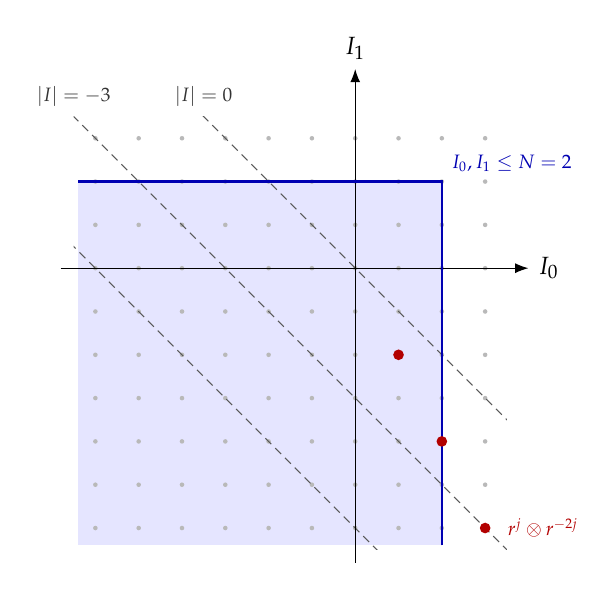
\begin{tikzpicture}[>=Latex,scale=0.55]
 \fill[blue!10] (-6.4,-6.4) rectangle (2,2);
 \foreach \a in {-6,...,3}{\foreach \c in {-6,...,3}{\fill[gray!55] (\a,\c) circle (1.5pt);}}
 \begin{scope}
  \clip (-6.5,-6.5) rectangle (3.5,3.5);
  \foreach \m in {0,-3,-6}{
    \draw[gray!70!black,densely dashed] (\m+7,-7) -- (\m-7,7);}
 \end{scope}
 \node[font=\scriptsize,gray!40!black,anchor=south] at (-3.5,3.5) {\(|I|=0\)};
 \node[font=\scriptsize,gray!40!black,anchor=south] at (-6.5,3.5) {\(|I|=-3\)};
 \draw[->] (-6.8,0)--(4.0,0) node[right] {\small \(I_0\)};
 \draw[->] (0,-6.8)--(0,4.6) node[above] {\small \(I_1\)};
 \draw[blue!70!black,thick] (2,-6.4)--(2,2)--(-6.4,2);
 \node[blue!70!black,font=\scriptsize,anchor=south west] at (2,2) {\(I_0,I_1\le N=2\)};
 \foreach \j in {1,2,3}{\pgfmathtruncatemacro{\jj}{-2*\j}
   \fill[red!70!black] (\j,\jj) circle (3.5pt);}
 \node[red!70!black,font=\scriptsize,anchor=west] at (3.3,-6) {\(r^j\otimes r^{-2j}\)};
\end{tikzpicture}
\caption[Two chain models: the lattice of multi-degrees]{Multi-degrees
\((I_0,I_1)\) of Hochschild \(1\)-chains of \(\cP\). A stage
\(\cP_N^{\hot2}\) of Model I contains the components in the shaded quadrant
\(I_0,I_1\le N\). The total order \(|I|\) is constant on the dashed anti-diagonals,
and each anti-diagonal meets the quadrant in finitely many points. The series
\(\sum_{j\ge1}r^j\otimes r^{-2j}\) (red, \(r\) homogeneous of degree \(1\)) has total orders
\(-j\to-\infty\). It is an element of Model II, but it lies in no stage of Model I,
because its first entries have unbounded order.}
\label{fig:lattice}
\end{figure}

The convergence proof of Proposition~\ref{prop:line} sums infinite series of
corrections, so it applies directly only to Model II. We prove in
Appendix~\ref{app:mixed} that Model I has the same homology
(Remark~\ref{rem:convergence}).

\section{The spectral sequence of a quantum algebra (BG \S1)}\label{sec:BG1}

\begin{whatdoes}
For a formal deformation of a commutative algebra we filter Hochschild chains
by powers of \(\hb\). The first page of the resulting spectral sequence is the
space of differential forms, and the first differential is \(-i\hb\,\delta\).
This is the theorem of \cite[\S1]{BG}. We prove it, with the constant, and
correct a normalization.
\end{whatdoes}

\subsection{Setup}\label{subsec:BG1setup}
Let \(A\) be a commutative algebra, either a polynomial algebra or \(\CI(X)\) for a
manifold \(X\), and let \(\star\) be a formal deformation of \(A\)
(Definition~\ref{def:deformation}), local if \(A=\CI(X)\). The Hochschild complex
of \(A\Lser{\hb}\) over \(K=\C\Lser{\hb}\) has chains
\[
 C^K_k=\bigl(A^{\hot(k+1)}\bigr)\Lser{\hb}=\Bigl\{\sum_{j\ge J}\hb^jc_j:\ c_j\in C_k(A)\Bigr\},
\]
since a \(K\)-multilinear map is determined by its values on \(A\). Write
\(b=\sum_{l\ge0}\hb^lb_l\), where \(b_l\) is the Hochschild-type operator built from
\(P_l\): \(b_l=\sum_i(-1)^id_i^{(l)}\), with \(d_i^{(l)}\) applying \(P_l\) to the entries
\(i\), \(i+1\) (and \(d_k^{(l)}\) to \(a_k,a_0\), in this order). In the language of
Section~\ref{sec:ss}, take the order of \(\hb^jc\) to be \(p=-j\). Then
\(C_{p,k}=\hb^{-p}C_k(A)\), orders are bounded above, the filtration
\(F_p=\hb^{-p}C_k(A)[[\hb]]\) is complete, and \(b_l\) lowers the order by \(l\).

The \(b_0\)-complex is the Hochschild complex of the commutative algebra \(A\).
So the first page is
\[
 E^1_{p,k}=\hb^{-p}\HH_k(A)\cong\hb^{-p}\Om^k(A)
\]
by Theorem~\ref{thm:HKRpoly} or Theorem~\ref{thm:connes}. This is part (1) of
BG's theorem. The isomorphism is the HKR map \(\chi\) of \eqref{eq:HKR}.

\subsection{The first differential}\label{subsec:d1}

\begin{theorem}[{\cite[\S1, Theorem]{BG}}]\label{thm:d1}
Let \(P_1(a,b)-P_1(b,a)=-i\{a,b\}\). Under \(\chi\), the differential
\(d^1:E^1_{p,k}\to E^1_{p-1,k-1}\) is \(-i\hb\,\delta\), where \(\delta=[\iota_\pi,d]\) is
the Koszul--Brylinski operator of Lemma~\ref{lem:deltaformula}.
\end{theorem}

For a quantum algebra in BG's sense, \(P_1=\{a,b\}/2i\), so
\(P_1(a,b)-P_1(b,a)=\{a,b\}/i=-i\{a,b\}\), and the theorem says \(d^1=(\hb/i)\delta\),
as in \cite{BG}.

\begin{proof}
It suffices to compute \(d^1\) on forms \(\theta=a_0\,da_1\wedge\dots\wedge da_k\), which
span \(\Om^k\) (for \(\CI(X)\), use a partition of unity and coordinate functions,
or an embedding of \(X\) in \(\R^N\)). By Lemma~\ref{lem:chi},
\(F=\operatorname{Alt}(a_0;a_1,\dots,a_k)\) is a \(b_0\)-cycle with \(\chi(F)=\theta\), so
\(d^1\theta=\hb\,\chi(b_1F)\).

Split \(P_1=S+\kappa\{\cdot,\cdot\}\) with \(S\) symmetric and \(\kappa=-i/2\).
Replacing \(P_1\) by \(S\) in \(b_1F\), the inner faces cancel in pairs (\(\sigma\) and
\(\sigma\circ(i\ i{+}1)\) have opposite signs) and the first and last faces cancel as
in the proof of Lemma~\ref{lem:chi}, now because
\(S(a_0,a_{\sigma(1)})=S(a_{\sigma(1)},a_0)\). So we may replace \(P_1\) by
\(\kappa\{\cdot,\cdot\}\). With the notation \(D_{jl}\) of the proof of
Lemma~\ref{lem:deltaformula}, \((k-1)!\,\chi(b_1F)\) is the sum of three
groups of terms.
\begin{enumerate}
\item The face \(d_0\): \(\kappa\sum_\sigma\sgn(\sigma)\{a_0,a_{\sigma(1)}\}\,
da_{\sigma(2)}\wedge\dots\wedge da_{\sigma(k)}\). Grouping by \(\sigma(1)=j\), whose
reorderings carry the sign \((-1)^{j-1}\), this is
\(\kappa(k-1)!\sum_j(-1)^{j-1}\{a_0,a_j\}D_{0j}\).
\item The face \((-1)^kd_k\): \((-1)^k\kappa\sum_\sigma\sgn(\sigma)\{a_{\sigma(k)},a_0\}\,
da_{\sigma(1)}\wedge\dots\wedge da_{\sigma(k-1)}\). Grouping by \(\sigma(k)=j\) (sign
\((-1)^{k-j}\)) and using antisymmetry, this equals the expression in (1).
\item The inner faces: \(\kappa\sum_\sigma\sgn(\sigma)\sum_{i=1}^{k-1}(-1)^ia_0\,
da_{\sigma(1)}\wedge\dots\wedge d\{a_{\sigma(i)},a_{\sigma(i+1)}\}\wedge\dots\wedge
da_{\sigma(k)}\). Moving \(d\{\cdot,\cdot\}\) to the front costs \((-1)^{i-1}\). For fixed
\(i\) and \((\sigma(i),\sigma(i+1))=(j,l)\) with \(j<l\), the sign of \(\sigma\) is
\((-1)^{j+l+1}\) times the sign of the induced ordering of the remaining
indices; the pair \((l,j)\) gives the same contribution, since both the bracket
and the sign change. Each \(i\) contributes
\(-2\kappa(k-2)!\sum_{j<l}(-1)^{j+l+1}a_0\,d\{a_j,a_l\}\wedge D_{jl}\), and there are
\(k-1\) values of \(i\).
\end{enumerate}
Dividing by \((k-1)!\),
\[
 \chi(b_1F)=2\kappa\Bigl(\sum_j(-1)^{j+1}\{a_0,a_j\}D_{0j}+\sum_{j<l}(-1)^{j+l}a_0\,
 d\{a_j,a_l\}\wedge D_{jl}\Bigr)=-i\,\delta\theta
\]
by Lemma~\ref{lem:deltaformula}.
\end{proof}

The proof shows that the symmetric part of \(P_1\), which depends on the choice
of quantization, drops out. Only the Poisson bracket survives. It also proves
\(\delta^2=0\) once more, since \((d^1)^2=0\).

\begin{correction}[Normalizations]\label{corr:normalization}
BG identify chains with forms through the diagram of \cite[\S1]{BG}: a chain
is first antisymmetrized, \(E(a_0,\dots,a_m)=\frac1{m!}\operatorname{Alt}(a_0;a_1,\dots,a_m)\),
and an antisymmetric chain is then sent to \(a_0\,da_1\wedge\dots\wedge da_m\). The
composite chains \(\to\) forms is \(\chi'=m!\,\chi\), and the inverse sends
\(\theta\) to \(E(a_0,\dots,a_m)\). With this identification the computation above
gives \(d^1=\frac{\hb}{i\,m}\delta\) on \(m\)-forms, not \(\frac\hb i\delta\). For example, for
\(m=2\) and \(E(a_0,a_1,a_2)=\frac12(a_0\otimes a_1\otimes a_2-a_0\otimes a_2\otimes a_1)\) one finds
directly
\[
 \chi'\bigl(b_1E(a_0,a_1,a_2)\bigr)=-\frac i2\bigl(\{a_0,a_1\}\,da_2-\{a_0,a_2\}\,da_1-
 a_0\,d\{a_1,a_2\}\bigr)=-\frac i2\,\delta(a_0\,da_1\wedge da_2).
\]
Likewise \(\chi'\circ B=(m+1)\,d\circ\chi'\) on \(m\)-chains, whereas
\(\chi\circ B=d\circ\chi\) (Proposition~\ref{prop:Bd}). The constants \(\hb/i\) for
\(d^1\) and \(1\) for \(B\) in \cite[\S\S1,3]{BG} are correct for the normalized map
\(\chi\) of \eqref{eq:HKR}. Since the factors are non-zero, no homology
computation is affected.
\end{correction}

\subsection{Examples}\label{subsec:BG1examples}

\begin{example}[Moyal on \(\R^2\)]\label{ex:moyalE2}
For \(A=\CI(\R^2)\) with the Moyal product, \(E^1_{p,k}=\hb^{-p}\Om^k(\R^2)\) and
\(d^1=-i\hb\delta\). By Section~\ref{subsec:poissonR2},
\(E^2_{p,k}=\hb^{-p}H_k(\Om(\R^2),\delta)\) is \(\hb^{-p}\C\,\omega\) for \(k=2\) and zero
otherwise. The same computation with polynomial coefficients (where
\(\R^2\) is replaced by polynomial forms and the polynomial Poincaré lemma is
used) is consistent with Theorem~\ref{thm:weyl} for \(n=1\): the class of \(\omega\)
corresponds, up to a non-zero factor, to the leading term
\(1\otimes x\otimes\pa-1\otimes\pa\otimes x\) of the cycle of Example~\ref{ex:weylcycle}. Indeed
\(\pa\) has symbol \(i\xi\), and \(\chi(1\otimes x\otimes\xi-1\otimes\xi\otimes x)=dx\wedge d\xi=-\omega\).
\end{example}

\begin{example}[The symbol algebra in one variable]
On \(\Tdot\R=\{(x,\xi):\xi\ne0\}\), homogeneous functions of degree \(p\) are
\(f_\pm(x)|\xi|^p\) on the two half-lines. The \(1\)-form \(\theta=f(x)|\xi|^{p}\,dx\) has
\(\delta\theta=\{f|\xi|^p,x\}=pf|\xi|^{p-1}\sgn\xi\). So \(\delta\) is injective on such forms
for \(p\ne0\), and these \(1\)-forms are killed at \(E^2\). This is the mechanism
behind the vanishing of \(E^2\) off the line \(p=k-n\) of Figure~\ref{fig:ss}.
\end{example}

\begin{discussion}
BG call Hochschild homology a ``semi-classical invariant'': it is determined
at first order in \(\hb\), by the Poisson structure alone, once the spectral
sequence is known to degenerate at \(E^2\). For a general formal deformation
there is no reason for \(d^2\), \(d^3\), \dots\ to vanish, and convergence must be
checked separately. What makes the conic case work is homogeneity, which is
the subject of the next section.
\end{discussion}

\section{Conic symplectic manifolds (BG \S2)}\label{sec:BG2}

\begin{whatdoes}
We prove BG's commutator identity \([\delta,\eps(\iota_Z\omega)]=\Lie_Z+c(n-k)\) for
conformal Hamiltonian fields, and deduce from it, with \(Z\) the radial
field, that the homology of \(\delta\) on homogeneous forms lives in a single
homogeneity. This is the step that puts \(E^2\) on a line. Then we treat BG's
theorem for smooth quantum algebras, including convergence.
\end{whatdoes}

\subsection{Conic symplectic manifolds}\label{subsec:conic}
\begin{definition}[{\cite[\S2]{BG}}]
A \emph{conic symplectic manifold} is a symplectic manifold \((X,\omega)\), of
dimension \(2n\), with a free action \(\rho_t\), \(t>0\), of the multiplicative group
\(\R_+\) such that \(\rho_t^*\omega=t\omega\). Its generator \(R\), defined by
\(\rho_t=\exp((\log t)R)\), satisfies \(\Lie_R\omega=\omega\).
\end{definition}

The basic example is \(X=\Tdot M\) with \(\rho_t(x,\xi)=(x,t\xi)\). In general put
\(\alpha=\iota_R\omega\). By Cartan's formula \(d\alpha=\Lie_R\omega-\iota_Rd\omega=\omega\), so \(\omega\)
is exact; on \(\Tdot M\), \(\alpha=\sum\xi_j\,dx_j\) is the canonical \(1\)-form. The
quotient \(S=X/\R_+\) is a manifold, and choosing a positive function \(r\)
homogeneous of degree \(1\) (with a partition of unity) gives
\(X\cong S\times(0,\infty)\). Figure~\ref{fig:cone} shows the model.

\begin{figure}[htbp]
\centering
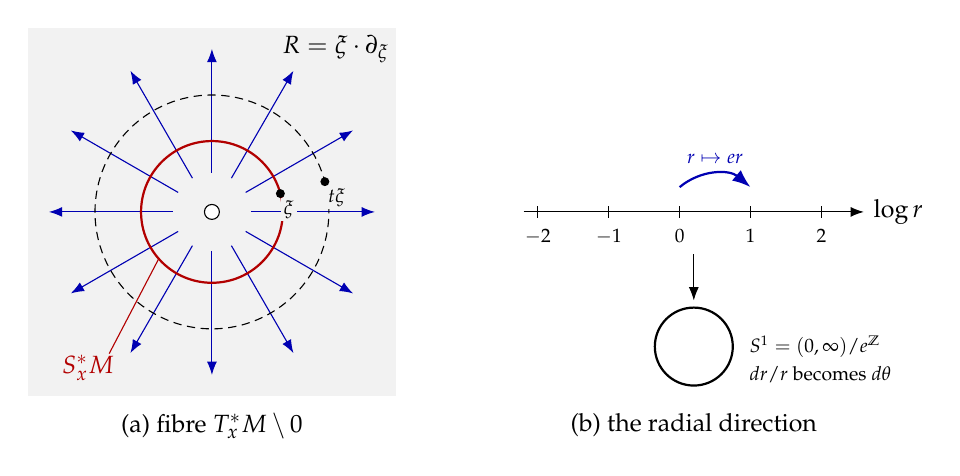
\begin{tikzpicture}[>=Latex,scale=0.9]
 \begin{scope}
  \fill[gray!10] (-2.6,-2.6) rectangle (2.6,2.6);
  \foreach \a in {0,30,...,330}{
    \draw[->,blue!70!black] ({0.55*cos(\a)},{0.55*sin(\a)}) -- ({2.3*cos(\a)},{2.3*sin(\a)});}
  \draw[thick,red!70!black] (0,0) circle (1);
  \draw[densely dashed] (0,0) circle (1.65);
  \fill[white] (0,0) circle (3pt); \draw (0,0) circle (3pt);
  \node[red!70!black,font=\small,fill=gray!10,inner sep=1pt] at (-1.75,-2.2) {\(S^*_xM\)};
  \draw[red!70!black,thin] (-1.45,-2.0) -- (-0.75,-0.66);
  \node[font=\small,fill=gray!10,inner sep=1pt] at (1.75,2.3) {\(R=\xi\cdot\pa_\xi\)};
  \node[font=\small,anchor=north] at (0,-2.7) {(a) fibre \(T^*_xM\setminus0\)};
  \fill ({cos(15)},{sin(15)}) circle (1.8pt); \fill ({1.65*cos(15)},{1.65*sin(15)}) circle (1.8pt);
  \node[font=\scriptsize,fill=gray!10,inner sep=1pt,anchor=north west] at ({cos(15)},{sin(15)-0.05}) {\(\xi\)};
  \node[font=\scriptsize,fill=gray!10,inner sep=1pt,anchor=north west] at ({1.65*cos(15)},{1.65*sin(15)-0.05}) {\(t\xi\)};
 \end{scope}
 \begin{scope}[xshift=6.6cm]
  \draw[->] (-2.2,0)--(2.6,0) node[right] {\small \(\log r\)};
  \foreach \x/\l in {-2/{-2},-1/{-1},0/0,1/1,2/2}{\draw (\x,-0.08)--(\x,0.08); \node[below,font=\scriptsize] at (\x,-0.1) {\(\l\)};}
  \draw[->,blue!70!black,thick] (0,0.35) to[bend left=40] node[above,font=\scriptsize]{\(r\mapsto er\)} (1,0.35);
  \draw[thick] (0.2,-1.9) circle (0.55);
  \draw[->] (0.2,-0.6)--(0.2,-1.25);
  \node[font=\scriptsize,anchor=west] at (0.85,-1.9) {\(S^1=(0,\infty)/e^{\Z}\)};
  \node[font=\scriptsize,anchor=west] at (0.85,-2.3) {\(dr/r\) becomes \(d\theta\)};
  \node[font=\small,anchor=north] at (0.2,-2.7) {(b) the radial direction};
 \end{scope}
\end{tikzpicture}
\caption[The conic symplectic cone and the radial field]{(a) A fibre of
\(\Tdot M\), with the radial vector field \(R\), the dilation \(\xi\mapsto t\xi\), and the
cosphere \(S^*_xM\) (any section of the rays would do). Homogeneous functions
are determined by their values on \(S^*_xM\). (b) In the coordinate
\(\log r\) dilation by \(e\) is translation by \(1\). Homogeneous forms of degree
\(0\) are invariant under it and descend to the circle \(S^1=(0,\infty)/e^{\Z}\), where
\(dr/r\) is the angular form. This is the circle of Theorem~\ref{thm:main}.}
\label{fig:cone}
\end{figure}

\begin{bgremark}[Darboux and the flow]\label{rem:darboux}
BG's conic Darboux lemma states that each point has a conic neighbourhood \(U\)
and a symplectomorphism \(\phi:U\to\Tdot\R^n\). This is an imprecision rather than an
error: what is used is that \(\phi\) can be chosen to \emph{commute with the dilations},
and that is not stated; its image is then an open conic subset of \(\Tdot\R^n\) (G6),
\cite[\S21.1]{Hormander3}. Also BG write \(T_t=\exp tR\); the flow at time \(s\) of \(R\) is
dilation by \(e^s\), so \(T_t=\exp((\log t)R)\). For \(X=\Tdot M\) we never need
the conic Darboux lemma: canonical coordinates are homogeneous Darboux
coordinates.
\end{bgremark}

A vector field \(Z\) is \emph{conformal Hamiltonian} if \(\Lie_Z\omega=c\,\omega\) for a
constant \(c\). Hamiltonian fields have \(c=0\), and \(R\) has \(c=1\). If \(Z\) has
constant \(c\), then \(Z-cR\) preserves \(\omega\), so it is locally Hamiltonian, and
\(Z=H_f+cR\) locally, as BG observe.

\subsection{The commutator identity}\label{subsec:commid}

\begin{theorem}[{\cite[\S2]{BG}}]\label{thm:commid}
Let \(Z\) be a conformal Hamiltonian vector field with \(\Lie_Z\omega=c\,\omega\). Then on
\(\Om^k(X)\)
\[
 [\delta,\eps(\iota_Z\omega)]=\delta\,\eps(\iota_Z\omega)+\eps(\iota_Z\omega)\,\delta=\Lie_Z+c\,(n-k).
\]
\end{theorem}

The bracket is the graded commutator; both operators are odd, so it is the
anticommutator. BG write \(\iota^*(Z)\) for \(\eps(\iota_Z\omega)\).

\begin{proof}
Write \(\theta=\iota_Z\omega\). We use the graded Jacobi identity for the even operator
\(\iota_\pi\) and the odd operators \(d\) and \(\eps(\theta)\):
\[
 [[\iota_\pi,d],\eps(\theta)]=[\iota_\pi,[d,\eps(\theta)]]-[d,[\iota_\pi,\eps(\theta)]].
\]
First, \([d,\eps(\theta)]=d\eps(\theta)+\eps(\theta)d=\eps(d\theta)\), since
\(d(\theta\wedge\beta)=d\theta\wedge\beta-\theta\wedge d\beta\). Here \(d\theta=d\iota_Z\omega=\Lie_Z\omega-
\iota_Zd\omega=c\,\omega\). By Lemma~\ref{lem:sl2}, \([\iota_\pi,\eps(c\,\omega)]=c(n-k)\) on
\(k\)-forms. Second, by \eqref{eq:iotapieps},
\([\iota_\pi,\eps(\theta)]=\iota_{\pi^\sharp\theta}\), and \(\pi^\sharp(\iota_Z\omega)=-Z\) because
\(\iota_{\pi^\sharp\eta}\omega=-\eta\) for every covector \(\eta\)
(Section~\ref{subsec:symplecticRn}). So \([d,\iota_{-Z}]=-(d\iota_Z+\iota_Zd)=-\Lie_Z\).
Putting the two together, \([\delta,\eps(\theta)]=c(n-k)+\Lie_Z\).
\end{proof}

\begin{corollary}\label{cor:commid}
\textup{(1)} For a function \(f\), \([\eps(df),\delta]=-\Lie_{H_f}\).
\textup{(2)} For the radial field, with \(\alpha=\iota_R\omega\),
\[
 [\delta,\eps(\alpha)]=\Lie_R+(n-k)\qquad\text{on }\Om^k .
\]
\end{corollary}

\begin{proof}
(1) Take \(Z=H_f\), \(c=0\), \(\iota_{H_f}\omega=-df\). (2) Take \(Z=R\), \(c=1\).
\end{proof}

\begin{bgremark}[The sign of the Hamiltonian identity]\label{rem:hamsign}
BG state \([\eps(df),\delta]=\Lie_{H_f}\). Their Hamiltonian field is defined by
\(H_gf=\{f,g\}\), which is our \(-H_g\), so the two statements agree. We checked
Theorem~\ref{thm:commid} for \(Z=R\) and \(Z=H_f\) symbolically on \(\R^4\), in all
degrees.
\end{bgremark}

BG prove Theorem~\ref{thm:commid} by conjugating \([d,\iota_Z]=\Lie_Z\) with their
star operator and expanding with the \(\mathfrak{sl}(2)\) relations; up to the
issues of Correction~\ref{corr:sl2}, this is the same computation as ours,
seen from the \(d\) side.

\subsection{Homogeneity: the homology of \texorpdfstring{\(\delta\)}{delta} lives in one degree}
\label{subsec:homog}
Let \(X\) be conic symplectic, and let \(\Om^k_{(p)}\) be the \(k\)-forms homogeneous of
degree \(p\). Since \(\pi\) is homogeneous of degree \(-1\), \(\delta\) maps
\(\Om^k_{(p)}\) to \(\Om^{k-1}_{(p-1)}\), and \(\eps(\alpha)\) maps \(\Om^k_{(p)}\) to
\(\Om^{k+1}_{(p+1)}\).

\begin{theorem}[{\cite[\S2]{BG}}]\label{thm:homog}
The homology of \(\Om^{k+1}_{(p+1)}\xrightarrow{\delta}\Om^k_{(p)}\xrightarrow{\delta}\Om^{k-1}_{(p-1)}\)
vanishes unless \(p=k-n\). For \(p=k-n\) it is isomorphic, by \(*\), to
\[
 H^{2n-k}(\Om^\bullet_{(0)},d)\cong H^{2n-k}(S)\oplus H^{2n-k-1}(S)\cong H^{2n-k}(S\times S^1),
 \qquad S=X/\R_+ .
\]
\end{theorem}

\begin{proof}
\emph{By the homotopy.} On \(\Om^k_{(p)}\), \(\Lie_R=p\), so Corollary~\ref{cor:commid}(2)
reads \(\delta\eps(\alpha)+\eps(\alpha)\delta=p+n-k\). If \(p\ne k-n\) and \(\delta\theta=0\), then
\(\theta=\delta(\alpha\wedge\theta)/(p+n-k)\), with \(\alpha\wedge\theta\in\Om^{k+1}_{(p+1)}\).
\emph{By the star.} By Theorem~\ref{thm:brylinski} and
Proposition~\ref{prop:starhom}, \(*\) carries the complex isomorphically onto
\(\Om^{2n-k-1}_{(c)}\to\Om^{2n-k}_{(c)}\to\Om^{2n-k+1}_{(c)}\), \(c=p+n-k\), with \(\delta\)
going to \(\pm d\). Proposition~\ref{prop:homdR}, whose proof applies to any
\(X\cong S\times(0,\infty)\), gives zero for \(c\ne0\) and the stated groups for \(c=0\).
\end{proof}

The two proofs are the same: under \(*\), the homotopy \(\eps(\alpha)\) becomes, up to
sign, the contraction \(\iota_R\) used in Proposition~\ref{prop:homdR}, by
Lemma~\ref{lem:starlemma}, and \(\pi^\sharp\alpha=-R\).

\begin{corollary}\label{cor:LRonH}
On all smooth forms, \(\Lie_R\) acts on the homology \(H_k(\Om^\bullet(X),\delta)\) as
multiplication by \(k-n\).
\end{corollary}

\begin{proof}
If \(\delta\theta=0\), then \((\Lie_R+n-k)\theta=\delta(\alpha\wedge\theta)\).
\end{proof}

\subsection{Degeneration: BG's homogeneity argument}\label{subsec:degen}
Let \(\star\) be a local conic star product on \(\CI(X)\Lser{\hb}\). BG's argument for
the vanishing of \(d^r\), \(r\ge2\), runs as follows. Let \(\Phi_t\) act on
\(\CI(X)\Lser{\hb}\) by \(\Phi_t(\hb^ja)=t^j\hb^j\rho_t^*a\). Since \(P_l\) lowers homogeneity
by \(l\), \(\Phi_t(a\star b)=\Phi_ta\star\Phi_tb\): \(\Phi_t\) is an automorphism over \(\C\)
(not over \(K\), since it rescales \(\hb\)). Its generator is the derivation
\(D=\hb\pa_\hb+\Lie_R\), which acts on chains, commutes with \(b\), and preserves the
filtration. On \(E^1_{p,k}=\hb^{-p}\Om^k\) it acts by \(-p+\Lie_R\), so on \(E^2_{p,k}\) it is the
scalar \(-p+k-n\) by Corollary~\ref{cor:LRonH}. The differential
\(d^r:E^r_{p,k}\to E^r_{p-r,k-1}\) commutes with \(D\), and \(D\) acts on source and
target by the scalars \(-p+k-n\) and \(-p+r+k-1-n\). These differ by \(r-1\), so
\((r-1)d^r=0\), and \(d^r=0\) for \(r\ge2\).

This is correct, but it uses the general pages \(E^r\) (G4), and it says nothing
about convergence. For the symbol algebra, homogeneity gives more: the
orders and the homogeneities are tied together, so \(E^2\) lies on a line and
Proposition~\ref{prop:line} applies (Section~\ref{sec:symbols}). For the
smooth quantum algebra we now give a direct proof of degeneration and
convergence.

\subsection{Smooth quantum algebras}\label{subsec:smoothquantum}
This subsection proves BG's corollary in \S2. It is not used later and can be
skipped.

\begin{theorem}[{\cite[\S2, Theorem and Corollary]{BG}}]\label{thm:smoothquantum}
Let \(X\) be a conic symplectic manifold of dimension \(2n\), \(S=X/\R_+\), and let
\(\star\) be a local conic star product on \(\CI(X)\Lser{\hb}\) with
\(P_1(a,b)-P_1(b,a)=-i\{a,b\}\). Then, as \(K\)-vector spaces,
\[
 \HH_k\bigl(\CI(X)\Lser{\hb}\bigr)\cong H^{2n-k}(X)\Lser{\hb}=H^{2n-k}(S)\Lser{\hb}.
\]
\end{theorem}

\begin{proof}
By Section~\ref{sec:BG1}, with Connes' theorem for the non-compact manifold \(X\)
(Theorem~\ref{thm:connes}), \(E^1_{p,k}=\hb^{-p}\Om^k(X)\) and \(d^1=-i\hb\delta\). By
Theorem~\ref{thm:brylinski} and de Rham's theorem,
\(E^2_{p,k}\cong\hb^{-p}H^{2n-k}(X)\). The filtration is complete. By
Proposition~\ref{prop:criterion} it suffices to prove (S) at every \((p,k)\).

\emph{The weight subcomplexes.} Write \(X\cong S\times(0,\infty)_r\). For \(\lambda\in\Z\),
let \(W^\lambda_k\) be the chains \(\sum_{j\ge J}\hb^jc_j\) with
\(c_j\in\bigoplus_{|I|=\lambda-j}\CI_{(I)}(X^{k+1})\) (finite sums of multi-homogeneous
functions). Since \(b_l\) lowers total homogeneity by \(l\) and comes with \(\hb^l\),
\(W^\lambda\) is a subcomplex, and it is complete. By Corollary~\ref{cor:HKRpoly}
(applied to \(\CI(S)\otimes\C[r^{\pm1}]\)) its first page at \(\hb^j\) is
\(\hb^j\Om^k_{(\lambda-j)}(X)\), with \(d^1=-i\hb\delta\) by the same proof. By
Theorem~\ref{thm:homog}, its second page vanishes unless \(\lambda-j=k-n\), that is,
unless the order \(p=-j\) equals \(k-n-\lambda\). So Proposition~\ref{prop:line}
applies to \(W^\lambda\), with \(n\) replaced by \(n+\lambda\), and every \(E^2\) class of
\(W^\lambda\) is the leading term of a cycle of \(W^\lambda\).

\emph{(S) for the smooth complex.} Let \(\xi\in E^2_{p,k}\), corresponding to a class
in \(H^{2n-k}(X)\). Represent that class by a form pulled back from \(S\), which
is homogeneous of degree \(0\), and let \(\theta=*^{-1}\) of it; then
\(\theta\in\Om^k_{(k-n)}\), \(\delta\theta=0\), and \(\hb^{-p}\theta\) represents \(\xi\). Now
\(\hb^{-p}\theta\) defines a class in the second page of \(W^\lambda\),
\(\lambda=-p+k-n\), so there is a cycle \(z\) of \(W^\lambda\) with leading term
representing it. Since \(W^\lambda\) is a subcomplex of the smooth complex and
the HKR maps agree, \(z\) is a cycle of the smooth complex whose leading term
represents \(\xi\).

\emph{The answer.} By Proposition~\ref{prop:criterion},
\(F_pH_k/F_{p-1}H_k\cong\hb^{-p}V\), \(V=H^{2n-k}(X)\), the filtration on \(H_k\) is
exhaustive and separated. Choose, for a basis of \(V\), cycles in \(F_0\) whose
leading terms represent the basis vectors, and extend linearly to
\(s:V\to Z_k\). The map \(\Psi(\sum_{j\ge J}\hb^jv_j)=[\sum_j\hb^js(v_j)]\) is defined by
completeness and \(K\)-linear. It is injective: if \(v_J\ne0\), the class lies in
\(F_{-J}H_k\) with \(\Theta_{-J}\) equal to \([\hb^Jv_J]\neq0\). It is surjective: for
\(h\in F_pH_k\), subtracting \(\Psi(\hb^{-p}v)\) with \(\Theta_p(h)=\hb^{-p}v\) moves \(h\) into
\(F_{p-1}H_k\), and after infinitely many steps the difference between \(h\) and
\(\Psi\) of the accumulated series lies in every \(F_qH_k\), hence vanishes.
\end{proof}

\begin{remark}
The weight subcomplexes \(W^\lambda\) are the ``semiclassical'' form of the symbol
algebra: setting \(\hb=1\) identifies \(W^0\) with the Model II chains of \(\cP\)
when \(X=\Tdot M\). Their homology contains the extra classes \(dr/r\) and is
\(H^{2n-k}(S\times S^1)\). These classes die in the smooth complex, where
\(dr/r=d\log r\) is exact. Nest and Tsygan \cite{NestTsygan} prove that
\(\HH_*\) of any formal deformation quantization of a symplectic manifold
\(X\) is \(H^{2n-*}(X)\Lser{\hb}\), by a different method (G15).
\end{remark}

\section{Cyclic homology of quantum algebras (BG \S3)}\label{sec:BG3}

\begin{whatdoes}
We run the argument of the previous two sections for the cyclic complex.
The point is to choose the filtration so that Connes' operator \(B\) enters only
at second order. Then \(E^2\) is the Hochschild \(E^2\) with a polynomial variable
\(u\) adjoined, and the homogeneity argument goes through.
\end{whatdoes}

\subsection{The filtration}\label{subsec:cycfilt}
Let \(\star\) be a formal deformation of \(A\), as in Section~\ref{sec:BG1}, and
consider the cyclic complex \(CC^K_N=\bigoplus_{j\ge0}C^K_{N-2j}u^j\) over \(K\), with
\(b+u^{-1}B\) (Section~\ref{subsec:bB}). BG use the differential
\(b+i^{-1}\hb^2u^{-1}B\) instead; the substitution \(u\mapsto i\hb^{-2}u\) identifies the
two complexes, since \(i^{-1}\hb^2\) is invertible in \(K\). In our language this
amounts to giving \(u\) the order \(2\):
\[
 \operatorname{order}(\hb^mc\,u^j)=-m+2j .
\]
Then \(b=\sum_l\hb^lb_l\) lowers order by \(l\) as before, while \(B\), which inserts the
unit and permutes cyclically, preserves powers of \(\hb\), so \(u^{-1}B\) lowers order by
exactly \(2\). The filtration is complete. Write the total differential as
\(\sum_lD_l\), with \(D_l\) lowering order by \(l\):
\[
 D_0=b_0,\qquad D_1=\hb b_1,\qquad D_2=\hb^2b_2+u^{-1}B,\qquad D_l=\hb^lb_l\ (l\ge3).
\]

\begin{lemma}[{\cite[\S3, Lemma]{BG}}]\label{lem:BG3}
\textup{(1)} The first page is \(E^1=\HH_*(A)\Lser{\hb}[u]\cong\Om^*(A)\Lser{\hb}[u]\), and
\(d^1=-i\hb\,\delta\) on each coefficient of \(u^j\).
\textup{(2)} Under the HKR map, \(B\) corresponds to the de Rham differential \(d\).
\end{lemma}

\begin{proof}
(1) \(D_0=b_0\) acts separately on each coefficient of \(u^j\), and \(D_1=\hb b_1\);
apply Theorem~\ref{thm:d1}. (2) is Proposition~\ref{prop:Bd}.
\end{proof}

So \(E^2=H_*(\Om,\delta)\Lser{\hb}[u]\), and the de Rham differential, carried by
\(u^{-1}B\), would first appear in \(d^2\).

\subsection{The conic case}\label{subsec:BG3conic}

\begin{theorem}[{\cite[\S3, Theorem and Corollary]{BG}}]\label{thm:BG3}
In the situation of Theorem~\ref{thm:smoothquantum}, the spectral sequence of
the cyclic complex degenerates at \(E^2\), converges, and
\[
 \HC_N\bigl(\CI(X)\Lser{\hb}\bigr)\cong\bigoplus_{j\ge0}H^{2n-N+2j}(X)\Lser{\hb}\,u^j .
\]
\end{theorem}

\begin{proof}
By Lemma~\ref{lem:BG3} and Theorem~\ref{thm:homog},
\(E^2_{q,N}=\bigoplus_j u^j\hb^{-p_j}H^{2n-N+2j}(X)\), where \(q=p_j+2j\). The proof of
Theorem~\ref{thm:smoothquantum} applies word for word. The weight subcomplexes
are spanned by \(\hb^mc\,u^j\) with \(c\) multi-homogeneous of total degree
\(\lambda-m\). In the weight-\(\lambda\) subcomplex the second page at
\(\hb^mc\,u^j\), with \(c\) of Hochschild degree \(N-2j\), is non-zero only if
\(\lambda-m=(N-2j)-n\), that is, only if the order \(-m+2j\) equals \(N-n-\lambda\).
So it lies on a line, Proposition~\ref{prop:line} gives (S), and
Proposition~\ref{prop:criterion} gives the result.
\end{proof}

\begin{bgremark}
In the proof of the theorem of \cite[\S3]{BG} the words are exchanged: the
argument given, that \(d^r\) changes homogeneity by \(-r\), proves
\emph{degeneration}, and convergence is what is referred back to
Section~2. Note also that, as in the Hochschild case, the homogeneity argument
needs representatives of homogeneity \(k-n\), which BG obtain from the homotopy
\([\delta,\eps(\alpha)]=\Lie_R+(n-k)\); this is Corollary~\ref{cor:LRonH}.
\end{bgremark}

\section{The homology of the symbol algebra (BG \S4)}\label{sec:symbols}

\begin{whatdoes}
We prove the main theorem: \(\HH_k(\cP)\cong H^{2n-k}(S^*M\times S^1)\), for both chain
models, and the analogous statement for cyclic homology. Then we express
the answer through the cohomology of \(M\) and correct BG's formula for this.
Throughout, \(M\) is closed, \(n=\dim M\ge1\), \(Y=\Tdot M\), and \(\cP\) carries the star
product of Proposition~\ref{prop:globalstar}.
\end{whatdoes}

\subsection{The first two pages}\label{subsec:PE1E2}
Filter Model I or Model II by total order (Lemma~\ref{lem:models}). In BG's
notation \(E^i_{kl}\) is our \(E^i_{l,k}\): \(k\) is the form degree and \(l\) the
homogeneity.

\begin{theorem}\label{thm:PE1}
For both models, \(\chi\) induces \(E^1_{p,k}\cong\Om^k_{(p)}(Y)\), the \(k\)-forms on \(Y\)
homogeneous of degree \(p\).
\end{theorem}

\begin{proof}
The associated graded complex is \(\bigoplus_mC_{m,\bullet}\) with \(b_0\), the Hochschild
complex of the commutative algebra \(\bigoplus_j\CI_{(j)}(Y)\) (finite sums). Choose a
positive \(r\in\CI_{(1)}(Y)\), so that \(\CI_{(j)}(Y)=r^j\CI(S^*M)\) and this algebra is
\(\CI(S^*M)\otimes\C[r^{\pm1}]\), with chains
\(\CI((S^*M)^{k+1})\otimes\C[r_0^{\pm1},\dots,r_k^{\pm1}]=\bigoplus_mC_{m,k}\). By
Corollary~\ref{cor:HKRpoly}, \(\chi\) identifies its homology with
\(\Om^k(S^*M)\otimes\C[r^{\pm1}]\oplus\Om^{k-1}(S^*M)\otimes\C[r^{\pm1}]\,dr\), preserving the
degree in \(r\). The part of degree \(p\) consists of the forms
\(r^p(\theta'+\theta''\wedge dr/r)\), which are exactly the homogeneous \(k\)-forms of degree \(p\).
\end{proof}

\begin{theorem}\label{thm:PE2}
\(d^1=-i\delta\) under \(\chi\), and
\[
 E^2_{p,k}\cong\begin{cases}H^{2n-k}(S^*M\times S^1)\cong H^{2n-k}(S^*M)\oplus H^{2n-k-1}(S^*M),&p=k-n,\\
 0,&p\ne k-n.\end{cases}
\]
\end{theorem}

\begin{proof}
The proof of Theorem~\ref{thm:d1} is a computation with the leading
homogeneous terms and applies verbatim, with \(\hb=1\). Then
Theorem~\ref{thm:homog}, with \(X=Y\) and \(S=S^*M\), computes \(E^2\).
\end{proof}

In words: \(E^2\) lies on the line \(p=k-n\) of Figure~\ref{fig:ss}. A Hochschild
\(k\)-cycle is detected by its term of total order \(k-n\). For \(k=0\) this is the term
of order \(-n\), which is the term the residue sees.

\begin{figure}[htbp]
\centering
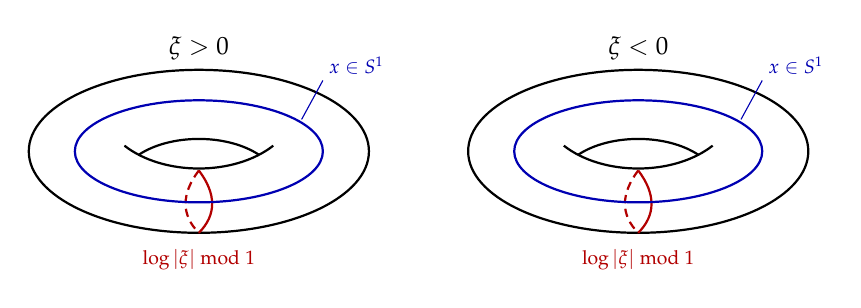
\begin{tikzpicture}[>=Latex,scale=0.9]
 \foreach \xs/\lab in {0/{\(\xi>0\)},6.2/{\(\xi<0\)}}{
 \begin{scope}[xshift=\xs cm]
  \draw[thick] (0,0) ellipse (2.4 and 1.15);
  \draw[thick] (-1.05,0.08) .. controls (-0.5,-0.35) and (0.5,-0.35) .. (1.05,0.08);
  \draw[thick] (-0.85,-0.05) .. controls (-0.4,0.25) and (0.4,0.25) .. (0.85,-0.05);
  \draw[red!70!black,thick] (0,-0.27) .. controls (0.25,-0.6) and (0.25,-0.9) .. (0,-1.15);
  \draw[red!70!black,thick,densely dashed] (0,-0.27) .. controls (-0.25,-0.6) and (-0.25,-0.9) .. (0,-1.15);
  \draw[blue!70!black,thick] (0,0) ellipse (1.75 and 0.72);
  \node[font=\small] at (0,1.45) {\lab};
  \node[blue!70!black,font=\scriptsize,anchor=south west] at (1.7,0.95) {\(x\in S^1\)};
  \draw[blue!70!black,thin] (1.75,1.0) -- (1.45,0.45);
  \node[red!70!black,font=\scriptsize,anchor=north] at (0,-1.25) {\(\log|\xi|\bmod1\)};
 \end{scope}}
\end{tikzpicture}
\caption[\(S^*M\times S^1\) for the circle]{\(S^*M\times S^1\) for \(M=S^1\). The cosphere bundle
\(S^*S^1=S^1\times\{\xi>0\}\sqcup S^1\times\{\xi<0\}\) is two circles (blue), and the radial
circle \(S^1=(0,\infty)/e^{\Z}\) (red) turns each into a torus. So \(\HH_k(\cP(S^1))\cong
H^{2-k}(T^2\sqcup T^2)\) has dimensions \(2,4,2\) for \(k=0,1,2\)
(Section~\ref{subsec:exS1}).}
\label{fig:SMS1}
\end{figure}

\subsection{The main theorem}\label{subsec:mainHH}

\begin{theorem}[{\cite[\S4, Theorem (1)]{BG}}]\label{thm:HHP}
For both chain models,
\[
 \HH_k(\cP)\cong H^{2n-k}(S^*M\times S^1)\cong H^{2n-k}(S^*M)\oplus H^{2n-k-1}(S^*M).
\]
More precisely, every class in \(\HH_k(\cP)\) has a representative \(c\) of total order
\(\le k-n\), and \([c]\mapsto[\chi(c_{k-n})]\in E^2_{k-n,k}\) is an isomorphism. In
particular \(\HH_k(\cP)=0\) for \(k>2n\).
\end{theorem}

\begin{proof}
For Model II the filtration is complete (Lemma~\ref{lem:models}), and
Theorem~\ref{thm:PE2} puts \(E^2\) on the line \(p=k-n\). Proposition~\ref{prop:line}
gives the result. For Model I, Theorem~\ref{thm:modelI} of
Appendix~\ref{app:mixed} shows that the inclusion into Model II induces an
isomorphism on homology compatible with the leading-term maps.
\end{proof}

\begin{corollary}\label{cor:HH0}
\(\HH_0(\cP)\cong H^{2n-1}(S^*M)\cong\C^{c}\), where \(c\) is the number of components of
\(S^*M\). If \(M\) is connected and \(n\ge2\), then \(c=1\). If \(n=1\), each component of \(M\)
gives two components of \(S^*M\).
\end{corollary}

\begin{proof}
\(H^{2n}(S^*M)=0\) for dimension reasons, and \(S^*M\) is a closed orientable manifold
(Lemma~\ref{lem:Sorient}), so \(H^{2n-1}(S^*M)\) has dimension equal to the number
of components. For \(n\ge2\) the fibre \(S^{n-1}\) is connected.
\end{proof}

\begin{bgremark}[Convergence and chain models]\label{rem:convergence}
BG prove convergence as follows \cite[\S\S2,4]{BG}. They observe that the
second page of the quotient complexes \(C/F_mC\) stabilizes as \(-m\to\infty\) (they
write ``\(m\) sufficiently large''), that \(C\) is the projective limit of the
\(C/F_mC\), and they invoke Grothendieck's Mittag-Leffler theorem with an
induction on the page. Two points are left open.
\begin{enumerate}
\item The homology of a projective limit of complexes is the projective limit of
the homologies only if the \(\varprojlim^1\) of the homologies in one degree higher
vanishes. This needs a Mittag-Leffler condition on the system
\(H_{k+1}(C/F_mC)\), which BG do not verify. Proposition~\ref{prop:line} is a
direct substitute: steps (P) and the completeness of the filtration supply
exactly the needed control.
\item The statement ``\(C\) is the projective limit'' holds for Model II, which is
the completion of Model I, but not for Model I, the chains
\(\varinjlim_N\cP_N^{\hot(k+1)}\) used elsewhere in the literature
\cite{MN,BN}; see Figure~\ref{fig:lattice}. For Model I one needs a separate
argument, given in Appendix~\ref{app:mixed} following Melrose--Nistor. Its result
is that the two models have the same homology.
\end{enumerate}
In later work on manifolds with boundary \cite{MN,LauterMoroianu} this point
is a genuine difficulty: for the symbol algebras with Laurent coefficients at the
boundary, the step-by-step argument inside a fixed stage, used in
Appendix~\ref{app:mixed}, is not available, and other methods are needed. On a closed
manifold there is no such problem.
\end{bgremark}

\subsection{Cyclic and periodic cyclic homology}\label{subsec:HCP}
For cyclic homology BG filter \(\cP[u]\) by \(F_m(\cP[u])=\sum_ju^jF_{m+2j}(\cP)\).

\begin{correction}[The filtration of \(\cP{[u]}\)]\label{corr:cyclicfilt}
This is not a filtration by subcomplexes. For \(c\in F_{m+2}(\cP)\),
\(uc\in F_m(\cP[u])\), but \((b+u^{-1}B)(uc)=(bc)u+Bc\), and \(Bc\in F_{m+2}(\cP)\) is not in
\(F_m(\cP)\) in general. The correct filtration, which matches the weight \(2\) of
\(u\) in Section~\ref{subsec:cycfilt} and the factor \(\hb^2\) in BG's \S3, is
\[
 F_q(CC_N(\cP))=\bigoplus_ju^j\,F_{q-2j}\bigl(C_{N-2j}(\cP)\bigr),
\]
so that \(u^{-1}B\) lowers order by \(2\).
\end{correction}

\begin{theorem}[{\cite[\S4, Theorem (2)]{BG}}]\label{thm:HCP}
For both models,
\[
 \HC_N(\cP)\cong\bigoplus_{j\ge0}H^{2n-N+2j}(S^*M\times S^1)\,u^j .
\]
\end{theorem}

\begin{proof}
Use Model II and the filtration of Correction~\ref{corr:cyclicfilt}. The
cyclic complex \(CC_N=\bigoplus_{j=0}^{\lfloor N/2\rfloor}\Chat_{N-2j}u^j\) is a finite
sum of complete complexes, hence complete. As in Lemma~\ref{lem:BG3}, the
total differential is \(\sum_lD_l\) with \(D_0=b_0\), \(D_1=b_1\), \(D_2=b_2+u^{-1}B\). So
\(E^1_{q,N}=\bigoplus_ju^j\Om^{N-2j}_{(q-2j)}(Y)\) and \(d^1=-i\delta\) on each coefficient. By
Theorem~\ref{thm:PE2} the coefficient of \(u^j\) in \(E^2_{q,N}\) vanishes unless
\(q-2j=(N-2j)-n\), that is \(q=N-n\), and is \(H^{2n-N+2j}(S^*M\times S^1)\) then. So
\(E^2\) lies on the line \(q=N-n\), and Proposition~\ref{prop:line} applies. For
Model I, the inclusion into Model II is a map of mixed complexes and an
isomorphism on Hochschild homology (Theorem~\ref{thm:modelI}), hence on
cyclic homology by Lemma~\ref{lem:HHtoHC}.
\end{proof}

\begin{corollary}\label{cor:HPP}
The maps \(S:\HC_N(\cP)\to\HC_{N-2}(\cP)\) are surjective, with kernel the image of
\(\HH_N(\cP)\). Hence the \(SBI\) sequence splits into short exact sequences, and
\(\HP_0(\cP)\cong H^{\mathrm{ev}}(S^*M\times S^1)\), \(\HP_1(\cP)\cong H^{\mathrm{odd}}(S^*M\times S^1)\).
\end{corollary}

\begin{proof}
\(S\) maps \(u^jc\) to \(u^{j-1}c\), so it lowers the filtration of
Correction~\ref{corr:cyclicfilt} by \(2\) and maps the line \(q=N-n\) to the line
\(q-2=(N-2)-n\). The leading-term isomorphisms of Theorem~\ref{thm:HCP}
therefore intertwine \(S\) with the map that deletes the term \(u^0\) and lowers the
other powers of \(u\). This is onto, with kernel the \(u^0\) term, which is the image of
\(I\). For \(\HP\) use the Milnor sequence of Section~\ref{subsec:HP} (G10): the
\(\varprojlim^1\) term vanishes, and the inverse limit along \(S\) is
\(\bigoplus_iH^{N+2i}\), the even or odd cohomology.
\end{proof}

\subsection{The answer in terms of \texorpdfstring{\(M\)}{M}}\label{subsec:gysin}
BG add: ``In particular, if \(n>1\), this is isomorphic to
\(H^{n-*-1}(M)\oplus H^{n-*}(M)\).''

\begin{correction}[The cohomology of \(S^*M\)]\label{corr:gysin}
This is false in general, and not only because of the Euler class. BG state it for
every \(M\) with \(n>1\) (and for \(\cP_c\)). For \(k=0\) it gives
\(H^{n-1}(M)\oplus H^n(M)\), which contradicts BG's own \(\HH_0(\cP)\cong\C\) for connected
closed \(M\) whenever \(b_{n-1}(M)\ne0\); for \(M=T^2\) it gives \(H^1\oplus H^2=\C^3\) instead of
\(\C\), although the Euler class of \(T^2\) vanishes. For \(M=S^2\), \(S^*S^2\cong SO(3)\cong\R P^3\), whose real
cohomology is \(\C\) in degrees \(0\) and \(3\). So \(S^*S^2\times S^1\) has cohomology \(\C\) in degrees
\(0\), \(1\), \(3\), \(4\), and \(\dim\HH_k(\cP(S^2))=1,1,0,1,1\) for \(k=0,\dots,4\). BG's formula gives
\(1,1,1,0,0\). The correct statement comes from the Gysin sequence (G5) of the
sphere bundle \(S^*M\to M\), with fibre \(S^{n-1}\):
\[
 \cdots\to H^{j-n}(M;o)\xrightarrow{\ e\ }H^j(M)\xrightarrow{\pi^*}H^j(S^*M)\xrightarrow{\pi_*}
 H^{j-n+1}(M;o)\xrightarrow{\ e\ }H^{j+1}(M)\to\cdots,
\]
where \(o\) is the orientation local system of \(M\) and \(e\) is the Euler class of \(T^*M\).
If \(e=0\) in real cohomology, for instance if \(n\) is odd or if \(M\) is closed and
connected with \(\chi_{\mathrm{top}}(M)=0\), the sequence splits and
\[
 \HH_k(\cP)\cong H^{2n-k}(M)\oplus H^{2n-k-1}(M)\oplus H^{n-k+1}(M;o)\oplus H^{n-k}(M;o).
\]
When \(e\ne0\), classes cancel in pairs. In all cases
\(\sum_k(-1)^k\dim\HH_k(\cP)=\chi_{\mathrm{top}}(S^*M\times S^1)=0\). These statements are checked on
examples in Section~\ref{sec:examples}.
\end{correction}

\begin{bgremark}[Hypotheses]\label{rem:hyp}
(1) The uniqueness of the residue needs \(M\) connected and \(n\ge2\); BG say this in
the text preceding their proposition. (2) For non-compact \(M\), BG state the
results for the algebra \(\cP_c\) of symbols with compact support, with
\(H_c^{2n-*}(S^*M\times S^1)\). The proof above goes through with compactly supported
forms, provided the chains are built from the direct limit over compact sets
\(K\subset M\) of the corresponding Model II complexes, and Connes' theorem is used in
its compactly supported form. Since \(\cP_c\) has no unit, one also needs
H-unitality of \(\cP_c\) (Section~\ref{subsec:Hunital}) to identify the homology of
the bar-type complexes. We do not write out these modifications, and we do not
use the non-compact case. (3) Hochschild homology of the full algebra
\(\Psi^{\Z}(M)\) differs from that of \(\cP\) only in degrees \(0\) and \(1\), by Wodzicki
excision (G9) for the H-unital ideal \(\Psi^{-\infty}\).
\end{bgremark}

\section{The residue and the higher residues (BG \S4)}\label{sec:residue}

\begin{whatdoes}
By Corollary~\ref{cor:HH0}, \(\HH_0(\cP)\) is one-dimensional when \(M\) is connected and
\(n\ge2\). We construct the trace that detects it, the non-commutative residue,
prove its local formula, and prove that \emph{every} trace on \(\cP\) is a multiple of
it, by an elementary argument with commutators. Then we compare normalizations
with \cite{BG}, relate the residue to residues of zeta functions, and explain
the higher residues as functionals on \(\HH_m(\cP)\).
\end{whatdoes}

\subsection{Traces and \texorpdfstring{\(\HH_0\)}{HH0}}\label{subsec:tracesHH0}
A trace on \(\cP\) is a linear map \(\tau:\cP\to\C\) vanishing on commutators. In Model II,
\(\HH_0(\cP)=\cP/b(\Chat_1)\), and \(b(\Chat_1)\) contains the commutators, but also limits of
sums of commutators. BG call a trace \emph{continuous} if it is continuous for their
topology \(\varprojlim_m\varinjlim_n\Psi^n/\Psi^m\). Concretely, such a \(\tau\) factors through
\(\cP/F_m\) for some \(m\), and its restriction to each \(\CI_{(j)}(Y)\) is continuous.

\begin{lemma}\label{lem:conttrace}
A continuous trace vanishes on \(b(\Chat_1)\). So continuous traces are the linear
functionals on \(\HH_0(\cP)\) (Model II) that factor through some \(\cP/F_m\) and are
continuous on each \(\CI_{(j)}(Y)\).
\end{lemma}

\begin{proof}
Let \(c=\sum_{q\le Q}c_q\in\Chat_1\). Then \(\tau(bu)=\sum_{m<p\le Q}\tau((bu)_p)\) is a finite sum,
and \((bu)_p=\sum_lb_lu_{p+l}\) is finite. Each \(c_q\) is a finite sum of elements of
\(\CI_{(I)}(Y^2)\), on which \(\tau\circ b_l\) is continuous, and on the dense subspace of
algebraic tensors \(\tau\circ b\) vanishes since \(b(a\otimes a')=[a,a']\).
\end{proof}

\subsection{The local residue}\label{subsec:localres}
Let \(U\subset\R^n\) be open. Let \(\cP_c(U)\subset\cP(M)\), for \(U\) a chart of \(M\), or
\(\cP_c(U)\) for \(U\subset\R^n\), be the classes of operators whose Schwartz kernel has
compact support in \(U\times U\). By (G1), the left quantization identifies \(\cP_c(U)\)
with full symbols \(a\) with compact \(x\)-support, through \(a\mapsto P_a=[\Op(a)\psi]\),
where \(\psi\in\CI_c(U)\) equals \(1\) near the \(x\)-support of \(a\); a different \(\psi\) changes
\(\Op(a)\psi\) by a smoothing operator (G1(d)). The product is \(P_aP_{a'}=P_{a\#a'}\).

\begin{lemma}\label{lem:xDcomm}
Let \(\tilde\psi\in\CI_c(U)\) be equal to \(1\) near \(\supp\psi\). Then in \(\cP_c(U)\)
\[
 [\tilde\psi x_k,P_a]=iP_{\pa_{\xi_k}a},\qquad[\tilde\psi D_{x_k},P_a]=P_{D_{x_k}a}.
\]
\end{lemma}

\begin{proof}
On kernels, \((x_k-y_k)e^{i(x-y)\cdot\xi}=-i\pa_{\xi_k}e^{i(x-y)\cdot\xi}\), and integration by
parts in \(\xi\) gives \([x_k,\Op(a)]=i\Op(\pa_{\xi_k}a)\). Since \(\tilde\psi=1\) on the supports
involved, \([\tilde\psi x_k,\Op(a)\psi]=[x_k,\Op(a)]\psi\). Similarly
\(D_{x_k}\Op(a)=\Op(\xi_ka+D_{x_k}a)\) and \(\Op(a)D_{x_k}=\Op(a\xi_k)\), so
\([\tilde\psi D_{x_k},\Op(a)\psi]=\Op(D_{x_k}a)\psi+\Op(a)(D_{x_k}\psi)\). The last operator has
kernel supported where \(x\in\supp a\) and \(y\in\supp D\psi\), which are disjoint, so it is
smoothing.
\end{proof}

\begin{lemma}\label{lem:divergence}
If \(h\) is smooth on \(\R^n\setminus0\) and homogeneous of degree \(1-n\), then
\(\int_{S^{n-1}}\pa_{\xi_k}h\,dS=0\).
\end{lemma}

\begin{proof}
\(\pa_kh\) is homogeneous of degree \(-n\), so in polar coordinates
\(\int_{1\le|\xi|\le R}\pa_kh\,d\xi=\log R\int_{S^{n-1}}\pa_kh\,dS\). By the divergence theorem the
left side is \(\int_{|\xi|=R}h\,\frac{\xi_k}{R}\,dS_R-\int_{|\xi|=1}h\,\xi_k\,dS\), and since
\(h(R\theta)=R^{1-n}h(\theta)\) and \(dS_R=R^{n-1}dS\), the two terms are equal. So the right side
vanishes for all \(R>1\). (For \(n=1\), \(S^0=\{\pm1\}\), \(h\) is constant on each half-line, and
\(\pa_\xi h=0\).)
\end{proof}

\begin{definition}
For \(a\) with compact \(x\)-support in \(U\), the \emph{local residue} is
\[
 \tau_U(P_a)=(2\pi)^{-n}\int_U\int_{|\xi|=1}a_{-n}(x,\xi)\,dS(\xi)\,dx .
\]
\end{definition}

\begin{proposition}\label{prop:localtrace}
\(\tau_U\) is a trace on \(\cP_c(U)\).
\end{proposition}

\begin{proof}
For functions \(f\), \(g\) and a first derivative \(\pa\), \(f\,\pa g=\pa(fg)-(\pa f)g\). Iterating,
\(f\,\pa^\beta g\equiv(-1)^{|\beta|}(\pa^\beta f)g\) modulo sums of first derivatives in the same
variables. Hence, modulo sums of \(\xi\)-derivatives and \(x\)-derivatives of products
of derivatives of \(a\) and \(a'\),
\[
 \pa_\xi^\alpha a\,D_x^\alpha a'\equiv(-1)^{|\alpha|}a\,\pa_\xi^\alpha D_x^\alpha a'\equiv
 (-1)^{|\alpha|}(-1)^{|\alpha|}(D_x^\alpha a)(\pa_\xi^\alpha a')=\pa_\xi^\alpha a'\,D_x^\alpha a .
\]
So every term of \(a\#a'-a'\#a=\sum_{\alpha\ne0}\frac1{\alpha!}(\pa_\xi^\alpha a\,D_x^\alpha a'-
\pa_\xi^\alpha a'\,D_x^\alpha a)\) is of the form \(\sum_k\pa_{x_k}G_k+\pa_{\xi_k}H_k\), with \(G_k\), \(H_k\)
finite sums of homogeneous terms with compact \(x\)-support. The term of degree \(-n\)
of \(\pa_{x_k}G_k\) integrates to zero over \(x\), and that of \(\pa_{\xi_k}H_k\) is
\(\pa_{\xi_k}\) of the term of degree \(1-n\) of \(H_k\), which integrates to zero over the sphere
by Lemma~\ref{lem:divergence}.
\end{proof}

\subsection{Uniqueness on a chart}\label{subsec:uniquechart}

\begin{proposition}\label{prop:uniquechart}
Let \(U\subset\R^n\) be connected and \(n\ge2\). Every trace \(\tau\) on \(\cP_c(U)\) is a multiple of
\(\tau_U\). No continuity is assumed.
\end{proposition}

\begin{proof}
Let \(\varpi(\xi)\) be smooth, \(0\) near \(0\) and \(1\) for \(|\xi|\ge1\). Products of \(\varpi\) with homogeneous
functions are classical symbols, and changing \(\varpi\) changes them by symbols of order
\(-\infty\), which are \(0\) in \(\cP\).

\emph{Step 1: degrees \(j\ne-n\).} Let \(p_j\) be homogeneous of degree \(j\) with compact
\(x\)-support. By Euler's identity \(\sum_k\pa_{\xi_k}(\xi_kp_j)=(j+n)p_j\). So
\(P_{\varpi p_j}=\sum_k\frac{-i}{j+n}[\tilde\psi x_k,P_{\varpi\xi_kp_j}]\) by Lemma~\ref{lem:xDcomm}, the
terms with \(\pa\varpi\) having order \(-\infty\). Hence \(\tau(P_{\varpi p_j})=0\). The same works for a
whole tail \(q\sim\sum_{j\le-n-1}q_j\): let \(b_k\) be a symbol with expansion
\(\sum_j\frac{-i}{j+n}\varpi\xi_kq_j\) (Borel); then \(P_q=\sum_k[\tilde\psi x_k,P_{b_k}]\) and \(\tau(P_q)=0\).
Since an element of \(\cP_c(U)\) has finitely many terms of degree \(>-n\), \(\tau\) depends
only on the term of degree \(-n\).

\emph{Step 2: degree \(-n\).} Let \(p\) be homogeneous of degree \(-n\) with compact
\(x\)-support, and \(\varrho(x)=\int_{S^{n-1}}p(x,\theta)\,dS\). Since \(n\ge2\), \(S^{n-1}\) is connected,
and Hodge theory on the round sphere (G5) gives \(w(x,\cdot)\), smooth in \(x\) with
compact support, with \(\Delta_Sw=p-\varrho/|S^{n-1}|\) on \(S^{n-1}\). Let \(g\) be the vector field on
\(\R^n\setminus0\), tangent to the spheres and homogeneous of degree \(1-n\), equal to
\(\nabla_Sw\) on \(S^{n-1}\). For a tangential field \(g(r\theta)=r^{1-n}V(\theta)\) one has
\(\operatorname{div}g=r^{-n}\operatorname{div}_SV\), so
\(\sum_k\pa_{\xi_k}g_k=|\xi|^{-n}\Delta_Sw=p-\varrho|\xi|^{-n}/|S^{n-1}|\). By Lemma~\ref{lem:xDcomm},
\(\tau(P_{\varpi p})=\tau(P_{\varpi\varrho|\xi|^{-n}})/|S^{n-1}|\). Next, fix \(\vartheta_0\in\CI_c(U)\) with
\(\int\vartheta_0=1\), and let \(\nu=\int_U\varrho\,dx\). Since \(U\) is connected, the compactly
supported function \(\varrho-\nu\vartheta_0\) has integral zero and so is
\(\sum_k\pa_{x_k}\beta_k\) with \(\beta_k\in\CI_c(U)\) (compactly supported de Rham cohomology in top
degree, G5). By Lemma~\ref{lem:xDcomm} again,
\[
 \tau(P_{\varpi p})=\nu\,\tau(P_{g_0}),\qquad g_0=\vartheta_0(x)\varpi(\xi)|\xi|^{-n}/|S^{n-1}| .
\]
Since \(\tau_U(P_{\varpi p})=(2\pi)^{-n}\nu\), we get \(\tau=c_U\tau_U\) on such elements, with
\(c_U=(2\pi)^n\tau(P_{g_0})\). With Step~1, \(\tau=c_U\tau_U\) on \(\cP_c(U)\).
\end{proof}

For \(n=1\) Step~2 fails: \(S^0\) has two points. Let \(U\subset\R\) be an interval and
\(\tau^\pm_U(P_a)=(2\pi)^{-1}\int_Ua_{-1}(x,\pm1)\,dx\). Each \(\tau^\pm_U\) is a trace, because the proof
of Proposition~\ref{prop:localtrace} works on each half-line \(\pm\xi>0\) separately
(Lemma~\ref{lem:divergence} for \(n=1\) says \(\pa_\xi h=0\)). Every trace \(\tau\) on \(\cP_c(U)\) is a
combination \(c_+\tau^+_U+c_-\tau^-_U\): Step~1 is unchanged, and a term of degree \(-1\) is
\(p=p_+(x)\mathbf 1_+|\xi|^{-1}+p_-(x)\mathbf 1_-|\xi|^{-1}\), with \(\mathbf 1_\pm\) the characteristic functions of \(\pm\xi>0\);
applying the \(x\)-part of Step~2 to \(p_+\) and \(p_-\) separately gives
\(\tau(P_{\varpi p})=\nu_+\tau(P_{g_+})+\nu_-\tau(P_{g_-})\), with \(\nu_\pm=\int p_\pm\,dx\) and
\(g_\pm=\vartheta_0(x)\varpi(\xi)\mathbf 1_\pm|\xi|^{-1}\).

\subsection{The global residue}\label{subsec:globalres}

\begin{lemma}\label{lem:Sintegral}
Let \(f\) be homogeneous of degree \(-n\) on \(\Tdot U\), with compact \(x\)-support. Then
\[
 \int_U\int_{|\xi|=1}f\,dS\,dx=\int_{S^*U}f\,\iota_R\vol ,
\]
where \(S^*U\) is oriented by \(\iota_R\vol\)
and identified with any section of the rays. In particular the left side does not
depend on the coordinates.
\end{lemma}

\begin{proof}
The form \(\iota_R(f\vol)\) is homogeneous of degree \(0\) and closed:
\(d\iota_R(f\vol)=\Lie_R(f\vol)-\iota_Rd(f\vol)=(-n+n)f\vol=0\). So its integral over a section of
the rays does not depend on the section (Stokes, with compact \(x\)-support). On
\(\{|\xi|=1\}\), \(|\iota_R\vol|=|\iota_R(d\xi_1\wedge\dots\wedge d\xi_n)|\,|dx|=dS\,dx\). A change of coordinates
induces a map of \(\Tdot U\) preserving \(\omega\), \(R\) and the principal symbol.
\end{proof}

\begin{theorem}[The residue]\label{thm:residue}
Let \(M\) be closed. There is a unique linear functional \(\res\) on \(\cP\) with
\(\res(\phi A)=\tau_U(\phi A)\) whenever \(\phi\in\CI_c(U)\) for a chart \(U\) and \(\phi A\in\cP_c(U)\) (with \(\phi A\)
replaced by \(\phi A\psi\), \(\psi=1\) near \(\supp\phi\)). It is a trace, and
\[
 \res(A)=(2\pi)^{-n}\int_{S^*M}\sigma(A)_{-n}\,\iota_R\Bigl(\frac{\omega^n}{n!}\Bigr),
\]
where \(\sigma\) is the global symbol of Proposition~\ref{prop:globalstar}. If \(A\) has
order \(\le-n\), \(\sigma(A)_{-n}\) is the principal symbol of order \(-n\).
\end{theorem}

\begin{proof}
\emph{Invariance on overlaps.} Let \(U\), \(U'\) be charts and \(B\subset U\cap U'\) a coordinate ball.
Then \(\tau_U\) and \(\tau_{U'}\) restrict to traces on \(\cP_c(B)\) (Proposition~\ref{prop:localtrace}),
so \(\tau_{U'}=c\,\tau_U\) there if \(n\ge2\) (Proposition~\ref{prop:uniquechart}). To find \(c\), take \(A\in\cP_c(B)\) of
order \(-n\) with \(\int_{S^*B}\sigma_{-n}(A)\iota_R\vol\ne0\). In both charts the term of degree
\(-n\) of the full symbol is the principal symbol (G1(c)), so by
Lemma~\ref{lem:Sintegral} \(\tau_U(A)=\tau_{U'}(A)\), and \(c=1\).

\emph{The case \(n=1\).} Fix an orientation of \(M\) (every \(1\)-manifold is orientable) and
use oriented charts only. A change of oriented coordinates \(x'=\phi(x)\), \(\phi'>0\),
sends \(\xi\) to \(\xi/\phi'(x)\), so it preserves the half-lines \(\pm\xi>0\). Now
\(\tau^+_{U'}=c_+\tau^+_U+c_-\tau^-_U\) on \(\cP_c(B)\). Testing on an element of order \(-1\) whose
principal symbol is supported in \(\xi<0\) gives \(c_-=0\), because \(\tau^+_{U'}\) vanishes on it
(the half-lines are preserved). Testing on one with principal symbol supported in
\(\xi>0\) and Lemma~\ref{lem:Sintegral}, applied on the half-line, gives \(c_+=1\). The same
holds for \(\tau^-\).

In all dimensions, then, by a partition of unity inside \(U\cap U'\), \(\tau_U=\tau_{U'}\) (respectively \(\tau^\pm_U=\tau^\pm_{U'}\)) on \(\cP_c(U\cap U')\).

\emph{Definition.} Choose charts \(U_i\) and a partition of unity \(\phi_i\), and put
\(\res(A)=\sum_i\tau_{U_i}(\phi_iA)\). By invariance on overlaps, inserting a second partition
of unity \(\phi'_j\) and writing \(\phi_iA=\sum_j\phi_i\phi'_jA\) shows that \(\res\) does not depend on
the choices. Since the full symbol of \(\phi_jA\) in the chart \(U_j\) is \(\phi_j\sigma_j(A)\),
\(\res(A)=(2\pi)^{-n}\sum_j\int\phi_j\sigma_j(A)_{-n}=\) the stated integral, by
Lemma~\ref{lem:Sintegral}.

\emph{Trace.} Choose the partition of unity so fine that whenever
\(\supp\phi_i\cap\supp\phi_j\ne\varnothing\), the union lies in one chart \(U_{ij}\) (Lebesgue number).
Then \([A,A']=\sum_{i,j}[\phi_iA,\phi_jA']\). If \(\supp\phi_i\cap\supp\phi_j=\varnothing\), both products
\(\phi_iA\phi_jA'\) and \(\phi_jA'\phi_iA\) are \(0\) in \(\cP\) by G1(d). Otherwise both factors lie in
\(\cP_c(U_{ij})\), after cutting off on the right, and \(\res([\phi_iA,\phi_jA'])=
\tau_{U_{ij}}([\phi_iA,\phi_jA'])=0\) by Proposition~\ref{prop:localtrace}.
\end{proof}

\begin{theorem}[Uniqueness]\label{thm:unique}
Let \(M\) be closed and connected. If \(n\ge2\), every trace on \(\cP\) is a multiple of \(\res\). If
\(n=1\), every trace is a combination of the two traces \(\res^\pm\), defined with \(\xi>0\) and
\(\xi<0\) respectively.
\end{theorem}

\begin{proof}
Let \(\tau\) be a trace. With charts \(U_i\) and a partition of unity, \(\tau(A)=\sum_i\tau(\phi_iA)\),
and \(\tau=c_i\tau_{U_i}\) on \(\cP_c(U_i)\) by Proposition~\ref{prop:uniquechart} (take connected
charts). If \(U_i\cap U_j\ne\varnothing\), testing on an element supported in a small ball
inside \(U_i\cap U_j\) with non-zero residue gives \(c_i=c_j\). Since \(M\) is connected, all
\(c_i\) agree, and \(\tau=c\,\res\). For \(n=1\), orient \(M\) and use oriented charts, so that
\(\xi>0\) and \(\xi<0\) are globally defined and preserved by changes of chart (proof of
Theorem~\ref{thm:residue}). On each chart \(\tau=c^+_i\tau^+_{U_i}+c^-_i\tau^-_{U_i}\). On an overlap,
testing on elements supported in a small ball with principal symbol supported in
\(\xi>0\) (respectively \(\xi<0\)) gives \(c^+_i=c^+_j\) (respectively \(c^-_i=c^-_j\)), and
connectedness gives \(\tau=c^+\res^++c^-\res^-\).
\end{proof}

\begin{remark}
BG prove uniqueness only among continuous traces, as a consequence of
\(\dim\HH_0(\cP)=1\). Theorem~\ref{thm:unique} is the algebraic statement of Wodzicki
\cite{Wodzicki-residue}; the proof above is the one used for the algebra of
operators in \cite{MN}. Melrose \cite[Ch.~10]{MelroseMicro} notes that the
algebraic statement needs an argument beyond the Hochschild computation, which
is what Steps~1 and~2 provide; see also \cite{LeschNeira}.
\end{remark}

\subsection{The residue and \texorpdfstring{\(\HH_0\)}{HH0}: normalizations}\label{subsec:resHH0}
By Lemma~\ref{lem:conttrace}, \(\res\) defines a functional on \(\HH_0(\cP)\). It is
continuous, since it only involves the term of degree \(-n\). We compare it with the
isomorphism of Theorem~\ref{thm:HHP}.

\begin{proposition}\label{prop:resTheta}
Let \(\Theta:\HH_0(\cP)\to E^2_{-n,0}\) be the leading-term isomorphism, followed by
\(*:E^2_{-n,0}\to H^{2n}(\Om_{(0)})\) and by \(H^{2n}(\Om_{(0)})\cong H^{2n-1}(S^*M)\),
\(\theta'+\theta''\wedge dr/r\mapsto[\theta'']\). Pairing with the fundamental class of \(S^*M\)
(oriented by \(\iota_R\vol\)) gives the functional \(-(2\pi)^n\res\).
\end{proposition}

\begin{proof}
Every class has a representative \(a\) of order \(\le-n\). Then \(\Theta[a]=[a_{-n}]\), and
\(*a_{-n}=a_{-n}\vol=\theta''\wedge dr/r\). Since \(\iota_R\theta''=0\) and \(\iota_R(dr/r)=1\),
\(\iota_R(a_{-n}\vol)=-\theta''\), so the pairing is \(-\int_{S^*M}a_{-n}\iota_R\vol=-(2\pi)^n\res(a)\).
\end{proof}

\begin{correction}[Constants in BG's Proposition]\label{corr:zeta}
(1) BG normalize \(R_M\) to take the value \(1\) on the orientation class of
\(H^{2n-1}(S^*M)\), show that it is proportional to \(\int_{S^*M}a_{-n}\,\iota(R)\omega^n\) (their
Prop.~(1) as printed has no constant), and end the proof with ``in fact, it can be
shown that \(c=2\pi\)''. It is not clear which \(c\) is meant. If it is the constant
relating \(R_M\) to the integral: The constant depends on the normalizations of the HKR map
(Correction~\ref{corr:normalization}), of the star operator
(Correction~\ref{corr:sl2}) and of the orientation, none of which is fixed in
\cite{BG}. With the conventions of these notes, Proposition~\ref{prop:resTheta}
gives \(R_M=-(2\pi)^n\res=-\frac1{n!}\int a_{-n}\iota_R\omega^n\), so the constant is \(-1/n!\). If
it is the \(c\) of their Prop.~(2), with \(R(P)=\int a_{-n}\iota(R)\omega^n\), then
Proposition~\ref{prop:zeta} gives \(c=(2\pi)^{-n}/(m\cdot n!)\), up to the orientation sign.
Neither is \(2\pi\).
(2) In BG's Proposition~(2), the constant in \(\Res_{s=0}\Tr(PA^{-s})=c\,R(P)\) depends
on the order \(m\) of \(A\), not only on \(\dim M\): by Proposition~\ref{prop:zeta},
\(\Res_{s=0}\Tr(PA^{-s})=\frac1m\res(P)\). For instance, replacing \(A\) by \(A^2\) halves the
left side, since \(\Tr(PA^{-2s})\) is the same function evaluated at \(2s\). Also \(A\)
must be invertible with spectrum in a sector for \(A^{-s}\) to be defined; positivity
of the principal symbol alone does not ensure invertibility.
\end{correction}

\subsection{Residues of zeta functions}\label{subsec:zeta}

\begin{lemma}[Seeley's computation \cite{Seeley}]\label{lem:seeley}
Let \(a(s;x,\xi)\) be a holomorphic family of classical symbols of order \(\mu(s)=k-ms\),
\(m>0\), with compact \(x\)-support: \(a=\sum_{j<J}a_{\mu-j}+r_J\), with \(a_{\mu-j}\) homogeneous of degree
\(\mu(s)-j\) for \(|\xi|\ge1\), holomorphic in \(s\), and \(|r_J|\le C|\xi|^{\operatorname{Re}\mu-J}\) locally
uniformly. Then \(I(s)=\int\!\!\int a(s;x,\xi)\,d\xi\,dx\), holomorphic for \(\operatorname{Re}\mu(s)<-n\),
extends meromorphically to \(\C\) with at most simple poles at the points where
\(\mu(s)=j-n\), and
\[
 \Res_{s=s_j}I=\frac1m\int\!\!\int_{|\xi|=1}a_{-n}(s_j;x,\xi)\,dS\,dx .
\]
\end{lemma}

\begin{proof}
Split \(\int_{|\xi|\le1}+\int_{|\xi|\ge1}\); the first is entire. In the second use polar coordinates:
\(\int_1^\infty r^{\mu-j+n-1}dr=\frac1{j-n-\mu(s)}=\frac{1/m}{s-s_j}\), for \(\operatorname{Re}\mu<j-n\), where
\(\mu(s_j)=j-n\). The remainder \(r_J\) contributes a function holomorphic for
\(\operatorname{Re}\mu<J-n\). Since \(J\) is arbitrary, this gives the continuation and the
residues.
\end{proof}

\begin{background}[Trace class and complex powers, (G8)]\label{bg:seeley}
(a) An operator in \(\Psi^\mu(M)\) with \(\operatorname{Re}\mu<-n\) is of trace class, and for
\(A=\phi\Op(a)\psi\) in a chart, \(\Tr A=(2\pi)^{-n}\int\!\!\int\phi\psi a\,d\xi\,dx\).
(b) If \(A\in\Psi^m(M)\), \(m\ge1\), is elliptic and invertible with principal symbol
positive (more generally with spectrum and principal symbol avoiding a ray),
then the complex powers \(A^{-s}\) of Seeley form a holomorphic family of order
\(-ms\) with \(A^0=1\), and for \(P\in\Psi^k(M)\) the local symbols of \(PA^{-s}\) are holomorphic
families of classical symbols as in Lemma~\ref{lem:seeley}, up to holomorphic
families of smoothing operators \cite{Seeley,Shubin}.
\end{background}

\begin{proposition}[Wodzicki, Guillemin]\label{prop:zeta}
In the situation of Background~\ref{bg:seeley}(b), \(\zeta(s)=\Tr(PA^{-s})\), defined for
\(\operatorname{Re}s>(k+n)/m\), extends meromorphically to \(\C\) with at most simple poles, and
\(\Res_{s=0}\zeta=\frac1m\res(P)\).
\end{proposition}

\begin{proof}
With a partition of unity and cut-offs, \(\Tr(PA^{-s})=\sum_i\Tr(\phi_iPA^{-s}\psi_i)\) plus
the trace of a holomorphic family of smoothing operators, whose kernels vanish
near the diagonal; that trace is entire. Apply Lemma~\ref{lem:seeley} to the local
symbol of \(\phi_iPA^{-s}\psi_i\), of order \(k-ms\). At \(s=0\) its term of degree \(-n\) is \(\phi_i\)
times the term of degree \(-n\) of the symbol of \(P\), since \(A^0=1\). By (G8)(a) and the lemma, the residue at \(s=0\) is
\(\frac1m(2\pi)^{-n}\sum_i\int\!\!\int_{|\xi|=1}\phi_ip^{(i)}_{-n}\,dS\,dx=\frac1m\res(P)\), where \(p^{(i)}\) is
the full symbol of \(P\) in the \(i\)-th chart.
\end{proof}

The functional \(\res\) is the \emph{Wodzicki--Guillemin residue}
\cite{Wodzicki-residue,Guillemin}; the factor \((2\pi)^{-n}\) is included by some
authors and not by others. BG mention that the trace was first observed by Adler
\cite{Adler} for \(M=\R\), in the theory of the KdV equation.

\subsection{Higher residues}\label{subsec:higher}
By Theorem~\ref{thm:HHP} and Poincaré duality on the closed oriented manifold
\(S^*M\) of dimension \(2n-1\),
\[
 \HH_m(\cP)^*\cong\bigl(H^{2n-m}(S^*M)\oplus H^{2n-m-1}(S^*M)\bigr)^*\cong H^{m-1}(S^*M)\oplus H^m(S^*M),
\]
which is BG's formula \(\HH^*(\cP)=H^{*-1}(S^*M)\oplus H^*(S^*M)\) for continuous Hochschild
cohomology. The functionals can be written down explicitly.

\begin{proposition}\label{prop:higher}
Let \(c\in F_{m-n}\Chat_m\) be a cycle, \(\theta=\chi(c_{m-n})\in\Om^m_{(m-n)}(Y)\), and
\(\gamma=*\theta\in\Om^{2n-m}_{(0)}\), which is closed. For closed forms \(\alpha\in\Om^m(S^*M)\) and
\(\beta\in\Om^{m-1}(S^*M)\) put
\[
 T_\alpha[c]=\int_{S^*M}\iota_R\gamma\wedge\alpha,\qquad T'_\beta[c]=\int_{S^*M}\gamma|_{S^*M}\wedge\beta .
\]
These are well-defined functionals on \(\HH_m(\cP)\), depending only on the classes of \(\alpha\)
and \(\beta\), and together they give the isomorphism above. Moreover, by
Lemma~\ref{lem:starlemma}, for \(\theta=f_0\,df_1\wedge\dots\wedge df_m\),
\[
 \iota_R*\theta=(-1)^{m(m+1)/2}f_0\,\iota_R\iota_{H_{f_1}}\cdots\iota_{H_{f_m}}\vol .
\]
\end{proposition}

\begin{proof}
Write \(\gamma=\gamma'+\gamma''\wedge dr/r\) as in Proposition~\ref{prop:homdR}. Then
\(\gamma|_{S^*M}=\gamma'\) and \(\iota_R\gamma=\pm\gamma''\), both closed on \(S^*M\). By
Theorem~\ref{thm:HHP}, \([c]\mapsto([\gamma'],[\gamma''])\) is an isomorphism onto
\(H^{2n-m}(S^*M)\oplus H^{2n-m-1}(S^*M)\). By Stokes' theorem on the closed manifold
\(S^*M\) the integrals depend only on the cohomology classes, and Poincaré duality says
that these pairings identify the dual space.
\end{proof}

For \(m=0\) and \(\alpha=1\) we recover \(T_1=\int_{S^*M}\iota_R(a_{-n}\vol)=(2\pi)^n\res\). BG's
formula for Wodzicki's higher residue \(\mathrm{Res}_m\) is the formula for \(\iota_R*\theta\) above,
with \(\eps^*(df)\) for \(\pm\iota_{H_f}\) and \(d\xi'\) for \(\iota_R\vol\).

\begin{bgremark}[The higher residue cochains]\label{rem:higherres}
BG write the Hochschild cochain attached to \(\alpha\) as
\((T\alpha)(a_0,\dots,a_m)=\int_{S^*M}\mathrm{Res}_m(a_0\,da_1\wedge\dots\wedge da_m)\wedge\alpha\), where
\(\mathrm{Res}_m\) keeps only the part of homogeneity \(m-n\). As a multilinear functional on \(\cP\)
this is not shown to be a Hochschild cocycle, and there is no reason to expect it to
be one: \((T\alpha)\circ b\) involves all the \(P_l\) through the components of \(b\) that land in
homogeneity \(m-n\), and only the \(b_0\) and \(b_1\) parts are controlled (the former by \(\chi\circ b_0=0\), the latter by \(d\alpha=0\) and Stokes). BG
describe \(T\alpha\) only through its image in the first page, and the precise
statement is Proposition~\ref{prop:higher}: the formula evaluates a class on its
representative of order \(\le m-n\). Note also that \(T\alpha\) only accounts for the summand
\(H^m(S^*M)\); the summand \(H^{m-1}(S^*M)\) comes from \(T'_\beta\).
\end{bgremark}

\section{Differential operators}\label{sec:diffops}

\begin{whatdoes}
The same spectral sequence computes the Hochschild homology of differential
operators. Here orders are \(\ge0\), so convergence is automatic, and the forms are
polynomial in \(\xi\), so the circle disappears: \(\HH_k(\cD(M))\cong H^{2n-k}(M)\). For a ball this
is BG's ``Poincaré lemma'', the input of the sheaf-theoretic method of
Section~\ref{sec:sheaf}. We also state the algebraic version of Kassel and
Mitschi.
\end{whatdoes}

\subsection{Differential operators on an open subset of \texorpdfstring{\(\R^n\)}{Rn}}\label{subsec:DU}
Let \(U\subset\R^n\) be open and \(\cD(U)\) the algebra of differential operators with smooth
coefficients, \(\cD(U)=\bigcup_N\cD^N(U)\), with \(\cD^N(U)\cong\CI(U)^{\binom{n+N}N}\) Fréchet.
The left symbol identifies \(\cD(U)\) with \(\CI(U)[\xi_1,\dots,\xi_n]\) as a vector space,
and for polynomial symbols the composition formula is exact:
\(a\#b=\sum_lP_l(a,b)\), a finite sum, with \(P_l(a,b)=\sum_{|\alpha|=l}\frac1{\alpha!}\pa_\xi^\alpha a\,D_x^\alpha b\).
The chains are \(\varinjlim_N\cD^N(U)^{\hot(k+1)}=\CI(U^{k+1})[\xi^{(0)},\dots,\xi^{(k)}]\) (G2), filtered by
total degree \(p\ge0\) in the \(\xi^{(j)}\). Each chain has finitely many components, so the
filtration is complete, and Proposition~\ref{prop:line} applies.

\begin{theorem}[{\cite[\S5]{BG}}]\label{thm:DU}
\(\HH_k(\cD(U))\cong H^{2n-k}(U)\). In particular, if \(U\) is a ball (BG's ``Poincaré
lemma''),
\[
 \HH_k(\cD(U))\cong\begin{cases}\C,&k=2n,\\0,&k\ne2n.\end{cases}
\]
The same holds for the Weyl algebra \(A_n\) of polynomial coefficient operators, with
\(U=\R^n\), in agreement with Theorem~\ref{thm:weyl}.
\end{theorem}

\begin{proof}
The associated graded algebra is \(\CI(U)\otimes\C[\xi]\). By
Corollary~\ref{cor:HKRpoly}, \(E^1_{p,k}\) is the space of \(k\)-forms on \(T^*U\) that are
polynomial in \(\xi\) and homogeneous of degree \(p\) (with \(d\xi_j\) of degree \(1\)). The proof
of Theorem~\ref{thm:d1} gives \(d^1=-i\delta\). The symplectic star has constant
coefficients, so it preserves polynomial forms, and by
Proposition~\ref{prop:homdR}(3) and Theorem~\ref{thm:brylinski}
\(E^2_{p,k}\cong H^{2n-k}(U)\) for \(p=k-n\) and \(0\) otherwise. Proposition~\ref{prop:line}
gives the result. For \(A_n\) replace \(\CI(U)\) by \(\C[x]\) and use
Theorem~\ref{thm:HKRpoly}; the polynomial Poincaré lemma gives \(H^*(\R^n)\).
\end{proof}

For \(U\) a ball the class in degree \(2n\) is represented, at leading order, by a chain
whose HKR image is \(*^{-1}1\), a multiple of \(\vol\); for \(n=1\) it is the cycle of
Example~\ref{ex:weylcycle}.

\begin{discussion}
Compare with symbols. For \(\cD\) the first page consists of forms polynomial in
\(\xi\), defined on all of \(T^*U\), including the zero section. A polynomial form of
homogeneity \(0\) cannot contain \(dr/r\), and it is just a form on \(U\). So the answer
is \(H^{2n-k}(U)\) with no circle. For symbols, which are only defined on \(\Tdot U\) and
are allowed negative homogeneity, \(dr/r\) is available and produces
\(H^{2n-k}(S^*U\times S^1)\). This is the contrast BG draw at the start of \S4, between
Laurent polynomial forms and smooth forms on the half-line.
\end{discussion}

\subsection{Differential operators on a manifold}\label{subsec:DM}

\begin{theorem}[{\cite[\S5]{BG}}; Wodzicki \cite{Wodzicki-cyclic}]\label{thm:DM}
For a manifold \(M\) without boundary, assuming (G11),
\[
 \HH_k(\cD(M))\cong H^{2n-k}(M),\qquad\HC_N(\cD(M))\cong\bigoplus_{j\ge0}H^{2n-N+2j}(M)\,u^j .
\]
\end{theorem}

\begin{proof}
The proof of Theorem~\ref{thm:DU} applies, once the first page is identified with
the forms on \(T^*M\) polynomial in the fibres, homogeneous of degree \(p\). This is the
HKR theorem for the algebra of fibrewise polynomial functions on \(T^*M\), which
is (G11). In a chart it is Corollary~\ref{cor:HKRpoly}, and the passage from local to
global is the partition-of-unity argument of Appendix~\ref{app:connes}, which we do
not write out for this algebra. For cyclic homology use the filtration of
Section~\ref{subsec:cycfilt}; orders are still \(\ge0\), and the argument of
Theorem~\ref{thm:HCP} applies.
\end{proof}

BG prove the Hochschild statement by the sheaf-theoretic method of
Section~\ref{sec:sheaf}, from the Poincaré lemma for balls, and remark that this
gives a second proof of the degeneration. With compact supports one obtains
\(H_c^{2n-*}(M)\) for \(\cD_c(M)\).

\subsection{Algebraic differential operators}\label{subsec:KM}

\begin{background}[Kassel--Mitschi {\cite{KasselMitschi}}, quoted in {\cite[\S5]{BG}}]
\label{bg:KM}
Let \(M\) be a smooth affine algebraic variety of pure dimension \(n\) over a field \(k\) of
characteristic \(0\), and \(\cD_{\mathrm{alg}}(M)\) the algebra of regular differential operators.
Then
\[
 \HH_*(\cD_{\mathrm{alg}}(M))\cong H^{2n-*}_{\mathrm{DR}}(M/k),\qquad
 \HC_*(\cD_{\mathrm{alg}}(M))\cong H^{2n-*}_{\mathrm{DR}}(M/k)[u].
\]
This is quoted by BG from a private communication; no proof is given in \cite{BG}.
\end{background}

BG sketch a proof for \(k=\C\). The map \(\cD_{\mathrm{alg}}(M)\to\cD_{\mathrm{an}}(M)\) into analytic
differential operators on the Stein manifold \(M\) respects the order filtrations, so
it induces a map of spectral sequences. On the second pages it is the map from
algebraic to analytic de Rham cohomology, which is an isomorphism by
Grothendieck's theorem \cite{Grothendieck}. Granting the convergence of both
spectral sequences, the two algebras have the same homology, and the analytic case
is computed as in Theorem~\ref{thm:DM}. The Lefschetz principle extends the
statement to fields of characteristic \(0\). All of this is (G14).

\begin{example}
For the affine line, \(\cD_{\mathrm{alg}}(\mathbb A^1)=A_1\) and \(H^*_{\mathrm{DR}}(\mathbb A^1)=k\) in degree \(0\).
The proposition gives \(\HH_2(A_1)=k\) and \(\HH_j(A_1)=0\) otherwise, in agreement with
Theorem~\ref{thm:weyl}. For \(\mathbb G_m=\operatorname{Spec}k[x,x^{-1}]\), \(H^0_{\mathrm{DR}}=H^1_{\mathrm{DR}}=k\), so the
proposition predicts \(\HH_2=\HH_1=k\) for the algebra generated by \(x^{\pm1}\) and \(\pa\).
\end{example}

\begin{remark}
Over \(\C\) the spectral sequence of this section also applies directly to
\(\cD_{\mathrm{alg}}(M)\), with the algebraic HKR theorem for the smooth affine variety
\(T^*M\), and gives the Kassel--Mitschi statement without passing through analytic
operators. We have not written out the details, and we do not use the
statement.
\end{remark}

\section{The sheaf-theoretic approach (BG \S5)}\label{sec:sheaf}

\begin{whatdoes}
BG's second method imitates Weil's proof of de Rham's theorem: a Poincaré lemma on
small open sets, plus a gluing argument. We first carry out Weil's proof completely
on the circle, then introduce sheaves only as far as needed, then explain BG's
argument for differential operators and its cyclic version, and finally the
microlocal version for symbols. The microlocal inputs are quoted.
\end{whatdoes}

\subsection{Weil's proof of de Rham's theorem on the circle}\label{subsec:weilS1}
Cover \(S^1\) by three open arcs \(U_0,U_1,U_2\) such that each \(U_{ij}=U_i\cap U_j\) (\(i<j\)) is a
non-empty arc and \(U_0\cap U_1\cap U_2=\varnothing\) (Figure~\ref{fig:weil}). Two arcs would not do:
their intersection would be two arcs, which is not connected. A cover by
contractible sets with contractible (or empty) intersections is called \emph{good}.

\emph{Čech cohomology.} Let \(\check C^0=\C^3\ni(f_0,f_1,f_2)\) (a constant on each arc),
\(\check C^1=\C^3\ni(g_{01},g_{02},g_{12})\) (a constant on each intersection), and
\(\check d(f)_{ij}=f_j-f_i\). The kernel of \(\check d\) consists of the constant triples, and the image is
two-dimensional. So \(\check H^0=\C\) and \(\check H^1=\C^3/\Ran\check d=\C\): the same as \(H^*_{\mathrm{dR}}(S^1)\). Weil's
theorem explains why.

\emph{The double complex.} Put \(K^{p,q}=\bigoplus_{|I|=p+1}\Om^q(U_I)\) for \(p=0,1\): forms on the arcs
(\(p=0\)) and on the intersections (\(p=1\)). There are two differentials, \(d\) on forms and
\(\check d\) (restriction and difference).

\begin{lemma}\label{lem:weilrows}
\textup{(Rows)} For each \(q\), \(0\to\Om^q(S^1)\to K^{0,q}\xrightarrow{\check d}K^{1,q}\to0\) is exact.
\textup{(Columns)} For each \(p\), \(K^{p,\bullet}\) has cohomology \(\check C^p\) in degree \(0\) (locally
constant functions, which are constant) and \(0\) in degree \(1\).
\end{lemma}

\begin{proof}
(Rows) Exactness at \(\Om^q(S^1)\) and at \(K^{0,q}\) says that forms agreeing on overlaps glue.
For surjectivity, take a partition of unity \(\rho_k\) subordinate to the cover, and given
\(\omega=(\omega_{ij})\), put \(\eta_i=\sum_k\rho_k\omega_{ki}\) on \(U_i\), with \(\omega_{ii}=0\) and \(\omega_{ki}=-\omega_{ik}\). On
\(U_{ij}\) the terms with \(k\notin\{i,j\}\) vanish, because \(U_k\cap U_{ij}=\varnothing\), so
\(\eta_j-\eta_i=\rho_i\omega_{ij}-\rho_j\omega_{ji}=(\rho_i+\rho_j)\omega_{ij}=\omega_{ij}\). (Columns) This is the
Poincaré lemma on arcs: a closed \(1\)-form on an interval is exact, and a function with
\(df=0\) on an interval is constant.
\end{proof}

Before the proof we recall three standard notions. A chain map \(f:C\to D\) is a
\emph{quasi-isomorphism} if it induces isomorphisms on all cohomology groups. Its
\emph{mapping cone} is the complex \(\mathrm{Cone}(f)^m=C^m\oplus D^{m-1}\) with differential
\((x,y)\mapsto(dx,f(x)-dy)\); there is a long exact sequence
\(\cdots\to H^{m-1}(D)\to H^m(\mathrm{Cone}(f))\to H^m(C)\xrightarrow{f}H^m(D)\to\cdots\), obtained from the
short exact sequence \(0\to D[-1]\to\mathrm{Cone}(f)\to C\to0\). So if \(f\) is onto with kernel
\(Z\), the inclusion \(Z\to\mathrm{Cone}(f)\), \(x\mapsto(x,0)\), is a quasi-isomorphism: the quotient
\(\mathrm{Cone}(f)/Z\) is the cone of the isomorphism \(C/Z\to D\) induced by \(f\), and the cone of
an isomorphism \(g\) is acyclic (a cycle \((x,y)\) has \(g(x)=dy\), and it is the boundary of
\((g^{-1}y,0)\)); then use the long exact sequence of \(0\to Z\to\mathrm{Cone}(f)\to\mathrm{Cone}(f)/Z\to0\). The \emph{five lemma} says that a map between two long exact
sequences that is an isomorphism at four out of every five consecutive places is an
isomorphism at the fifth. These are in any text on homological algebra
\cite[Ch.~1]{Weibel}.

\begin{theorem}[Weil, on the circle]\label{thm:weilS1}
\(H^*_{\mathrm{dR}}(S^1)\cong\check H^*(\{U_i\};\C)\).
\end{theorem}

\begin{proof}
Let \(T\) be the total complex, \(T^m=K^{0,m}\oplus K^{1,m-1}\), with differential
\((x,y)\mapsto(dx,\check d x-dy)\). This is the mapping cone of the chain map
\(\check d:K^{0,\bullet}\to K^{1,\bullet}\). By the rows, \(\check d\) is onto with kernel \(\Om^\bullet(S^1)\), so the
inclusion \(\Om^\bullet(S^1)\to T\), \(x\mapsto(x,0)\), is a quasi-isomorphism (a cone of a surjection is
quasi-isomorphic to its kernel). By the columns, the inclusions of constants
\(\check C^p\to K^{p,\bullet}\) are quasi-isomorphisms, so the induced map from the cone of
\(\check d:\check C^0\to\check C^1\), which computes \(\check H^*\), to \(T\) is a quasi-isomorphism by the five lemma
applied to the long exact sequences of the cones.
\end{proof}

\begin{figure}[htbp]
\centering
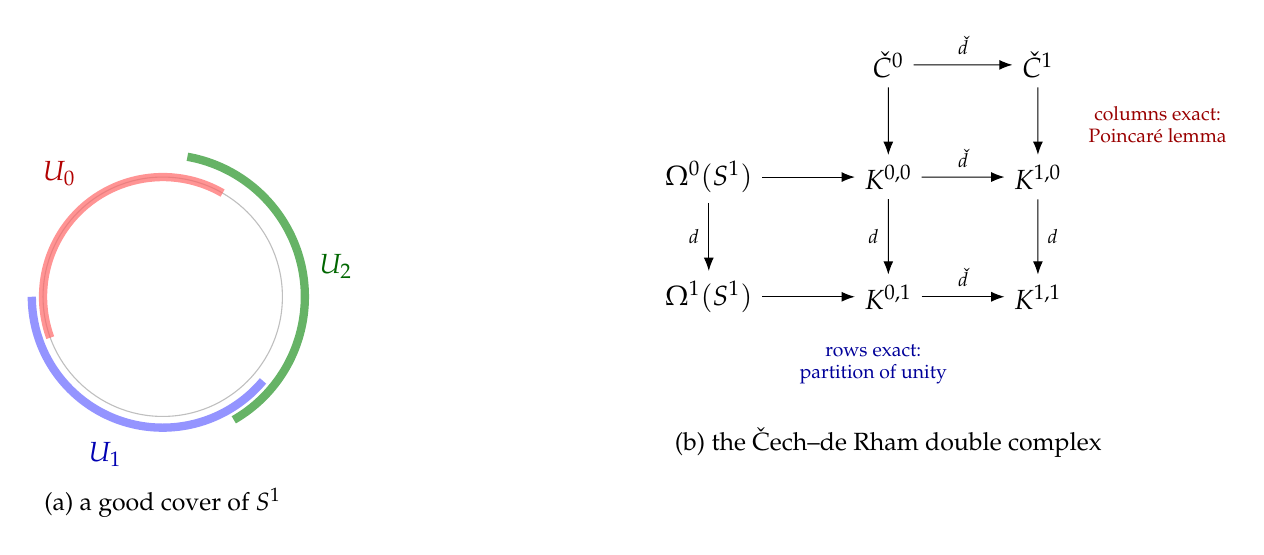
\begin{tikzpicture}[>=Latex,scale=0.95]
 \begin{scope}
  \draw[gray!50] (0,0) circle (1.6);
  \draw[line width=3pt,red!60,opacity=0.7] (60:1.6) arc (60:200:1.6);
  \draw[line width=3pt,blue!60,opacity=0.7] (180:1.75) arc (180:320:1.75);
  \draw[line width=3pt,green!50!black,opacity=0.6] (300:1.9) arc (300:440:1.9);
  \node[red!70!black] at (130:2.15) {\(U_0\)};
  \node[blue!70!black] at (250:2.25) {\(U_1\)};
  \node[green!40!black] at (10:2.35) {\(U_2\)};
  \node[font=\small] at (0,-2.75) {(a) a good cover of \(S^1\)};
 \end{scope}
 \begin{scope}[xshift=7.3cm,yshift=0.4cm,>=Latex]
  \node (a0) at (0,1.2) {\(\Om^0(S^1)\)};
  \node (a1) at (0,-0.4) {\(\Om^1(S^1)\)};
  \node (k00) at (2.4,1.2) {\(K^{0,0}\)};
  \node (k01) at (2.4,-0.4) {\(K^{0,1}\)};
  \node (k10) at (4.4,1.2) {\(K^{1,0}\)};
  \node (k11) at (4.4,-0.4) {\(K^{1,1}\)};
  \node (c0) at (2.4,2.7) {\(\check C^0\)};
  \node (c1) at (4.4,2.7) {\(\check C^1\)};
  \draw[->] (a0)--(k00); \draw[->] (k00)--node[above,font=\scriptsize]{\(\check d\)}(k10);
  \draw[->] (a1)--(k01); \draw[->] (k01)--node[above,font=\scriptsize]{\(\check d\)}(k11);
  \draw[->] (a0)--node[left,font=\scriptsize]{\(d\)}(a1);
  \draw[->] (k00)--node[left,font=\scriptsize]{\(d\)}(k01);
  \draw[->] (k10)--node[right,font=\scriptsize]{\(d\)}(k11);
  \draw[->] (c0)--(k00); \draw[->] (c1)--(k10);
  \draw[->] (c0)--node[above,font=\scriptsize]{\(\check d\)}(c1);
  \node[font=\scriptsize,align=center,blue!60!black] at (2.2,-1.3) {rows exact:\\ partition of unity};
  \node[font=\scriptsize,align=center,red!60!black] at (6.0,1.9) {columns exact:\\ Poincaré lemma};
  \node[font=\small] at (2.4,-2.35) {(b) the Čech--de Rham double complex};
 \end{scope}
\end{tikzpicture}
\caption[Weil's proof on the circle]{Weil's proof of de Rham's theorem on \(S^1\).
(a) Three arcs with connected pairwise intersections and empty triple
intersection. (b) Exact rows (gluing with a partition of unity) identify the total
cohomology with de Rham cohomology; exact columns (the Poincaré lemma on arcs)
identify it with Čech cohomology of constants. BG replace forms by Hochschild
chains of differential operators, and the Poincaré lemma by
Theorem~\ref{thm:DU}.}
\label{fig:weil}
\end{figure}

\subsection{Sheaves in a nutshell}\label{subsec:sheaves}
A \emph{presheaf} \(\mathcal F\) on \(M\) assigns a vector space \(\mathcal F(U)\) to each open set and
restriction maps \(\mathcal F(U)\to\mathcal F(V)\) for \(V\subset U\), compatible with composition. It is a
\emph{sheaf} if sections that agree on overlaps glue uniquely. Examples: \(\Om^q\)
(\(U\mapsto\Om^q(U)\)), the constant sheaf \(\C_M\) (locally constant functions), and
\(\cD_M\) (\(U\mapsto\cD(U)\)). The \emph{stalk} at \(x\) is \(\mathcal F_x=\varinjlim_{U\ni x}\mathcal F(U)\). Every
presheaf has a \emph{sheafification} with the same stalks. A sheaf is \emph{fine} if it
admits partitions of unity, as all \(\CI(M)\)-modules do; fine sheaves behave like the
rows of Lemma~\ref{lem:weilrows}. A morphism of complexes of sheaves is a
\emph{quasi-isomorphism} if it induces isomorphisms on the stalks of the cohomology
sheaves; Lemma~\ref{lem:weilrows}(columns) says that \(\C_M\to\Om^\bullet\) is one. The
\emph{hypercohomology} \(\mathbb H^*(M,\mathcal F^\bullet)\) of a complex of sheaves is the cohomology of the
total complex of the Čech double complex for a good cover (in general a limit over
covers), as in Theorem~\ref{thm:weilS1}.

\begin{background}[Weil's theorem in general, (G5), (G12)]\label{bg:weil}
(a) Quasi-isomorphic complexes of sheaves have isomorphic hypercohomology.
(b) If every \(\mathcal F^q\) is fine, \(\mathbb H^*(M,\mathcal F^\bullet)=H^*(\Gamma(M,\mathcal F^\bullet))\).
(c) \(\mathbb H^*(M,\C_M[m])=H^{*+m}(M;\C)\), where \([m]\) shifts degrees down by \(m\).
In particular \(H^*_{\mathrm{dR}}(M)=\mathbb H^*(M,\Om^\bullet)=\mathbb H^*(M,\C_M)=H^*(M;\C)\) \cite{BottTu,Weil}.
\end{background}

\subsection{Differential operators via sheaves}\label{subsec:Dsheaf}
BG's analogue \cite[\S5]{BG}: let \(\mathcal C^{-k}\) be the sheaf associated with the presheaf
\(U\mapsto C_k(\cD(U))\), so that \(\mathcal C^\bullet\) is a complex of sheaves in non-positive degrees, with
differential \(b\). Its cohomology sheaves have stalks
\(\varinjlim_{U\ni x}\HH_k(\cD(U))\). Balls are cofinal among neighbourhoods of \(x\), so by
Theorem~\ref{thm:DU} (the Poincaré lemma) the only non-zero cohomology sheaf is
\(\C_M\) in degree \(-2n\):
\[
 \mathcal C^\bullet\simeq\C_M[2n].
\]
Assuming that the global Hochschild complex computes the hypercohomology,
\(\HH_k(\cD(M))=\mathbb H^{-k}(M,\mathcal C^\bullet)=\mathbb H^{-k}(M,\C_M[2n])=H^{2n-k}(M)\), which is
Theorem~\ref{thm:DM}.

\subsection{Cyclic homology via sheaves}\label{subsec:cycsheaf}
Let \(\mathcal C^{\lambda,\bullet}\) be the analogous complex built from Connes' cyclic complex. By
Theorem~\ref{thm:DM} for balls (or Theorem~\ref{thm:DU} and the cyclic version of its
proof), \(\HC_N(\cD(U))=\C\) for \(N=2n+2j\), \(j\ge0\), and \(0\) otherwise, so the cohomology sheaves
of \(\mathcal C^{\lambda,\bullet}\) are \(\C_M\) in degrees \(-2n,-2n-2,\dots\) and zero otherwise.

\begin{proposition}[{\cite[\S5]{BG}}]\label{prop:cycsheaf}
In the derived category of sheaves on \(M\),
\(\mathcal C^{\lambda,\bullet}\simeq\bigoplus_{j\ge0}\C_M[2n+2j]\). Consequently, granting the identification of
global chains with hypercohomology, \(\HC_N(\cD(M))\cong\bigoplus_{j\ge0}H^{2n-N+2j}(M)\).
\end{proposition}

\emph{The following argument uses the derived category of sheaves (G12) and may be
skipped on a first reading.} Roughly, the derived category is obtained from
complexes of sheaves by declaring quasi-isomorphisms to be isomorphisms; in it a
complex whose cohomology sheaves are \(\C_M\) in a single degree is isomorphic to
\(\C_M\) shifted to that degree, and an exact sequence of complexes gives a
``distinguished triangle'', which splits when one of its maps has a one-sided
inverse. Nothing else from the theory is used.

\begin{proof}[Argument (in the derived category, (G12))]
Since \(-2n\) is the highest degree with a non-zero cohomology sheaf, there is a
truncation morphism \(t:\mathcal C^{\lambda,\bullet}\to\C_M[2n]\). The composite
\(t\circ I:\mathcal C^\bullet\to\mathcal C^{\lambda,\bullet}\to\C_M[2n]\) is a quasi-isomorphism: on stalks in degree
\(-2n\) it is \(I:\HH_{2n}(\cD(U))\to\HC_{2n}(\cD(U))\), which is an isomorphism for balls by the
\(SBI\) sequence, since \(\HC_{2n-1}\) and \(\HC_{2n-2}\) vanish there. Hence \(I\) has a left
inverse up to quasi-isomorphism, and \(\C_M[2n]\) is a direct summand of
\(\mathcal C^{\lambda,\bullet}\), with complement identified by \(S\) with \(\mathcal C^{\lambda,\bullet}[2]\). Induction on \(j\)
gives the statement.
\end{proof}

\begin{bgremark}[Gaps in the sheaf-theoretic argument]\label{rem:sheafgap}
(1) The presheaf \(U\mapsto C_k(\cD(U))\) assigns to \(U\) functions on \(U^{k+1}\), not on \(U\), so
its sections over \(U\cup V\) are not determined by those over \(U\) and \(V\). The step
``the global Hochschild complex computes the hypercohomology of \(\mathcal C^\bullet\)'' therefore
needs a \emph{localization} theorem: chains supported near the diagonal compute
Hochschild homology, and they form a complex of fine sheaves. This is true for
the algebras considered here (Teleman \cite{Teleman}; Brylinski
\cite{Brylinski-examples}), but it is not proved in \cite{BG}; it is (G12). (2) BG
write ``Hochschild cohomology'' where homology is meant. (3) In the cyclic
argument BG say that \(I\) is ``a left inverse to the map \(\C_M[2n]\to\mathcal C^{\lambda,*}\)''. The
morphisms go the other way, as above: the composite \(\mathcal C^\bullet\to\mathcal C^{\lambda,\bullet}\to\C_M[2n]\) is a
quasi-isomorphism. (4) Theorem~\ref{thm:DM} gives an independent proof of both
statements, modulo (G11).
\end{bgremark}

\subsection{Microdifferential operators}\label{subsec:micro}
For symbols, the Poincaré lemma must live on \(S^*M\times S^1\). BG obtain the circle from a
complexification. We describe the objects and quote the results.

\emph{Microdifferential operators} \cite{SKK,Kashiwara-book}. Let \(X\) be a complex
manifold of dimension \(n\). On \(T^*X\) there is a sheaf of rings \(\cE_X\), locally constant
along the orbits of \(\C^\times\) on \(\Tdot X\). A section over a conic open set is a formal sum
\(\sum_{j\le m}p_j(z,\zeta)\) of holomorphic functions homogeneous of degree \(j\) in \(\zeta\), subject to
a growth condition as \(j\to-\infty\) (on compact sets \(|p_j|\le C R^{-j}(-j)!\)). The product is
the composition formula \eqref{eq:intro-comp}, with \(\pa_\zeta\) and \(D_z\). So \(\cE_X\) is an analytic
version of \(\cP\). There are larger sheaves \(\cE^\infty_X\) (operators of infinite order) and
\(\cE_{\R}\) (defined through cohomology with supports; BG describe its stalks at
\((0,dz_1)\) by holomorphic kernels on wedge-shaped regions modulo kernels that
extend across one of the walls). The stalks of \(\cE_{\R}\) carry a product only modulo
such kernels; \(\cE^\infty=\pi'_*\cE_{\R}\).

\emph{Real symbols.} Let \(M\) be real analytic (every smooth closed manifold has a real
analytic structure) and \(M\hookrightarrow M_{\C}\) a complexification. Then
Figure~\ref{fig:complexify} commutes; \(i'\) is a closed immersion followed by an étale
map of degree \(2\). After a Riemannian metric is chosen, the \(\C^\times\)-bundle
\(\pi':\Tdot M_{\C}\to\Tdot M_{\C}/\C^\times\) trivializes over \(S^*M\), so
\(\pi'^{-1}(S^*M)\cong S^*M\times\C^\times\), which is homotopy equivalent to \(S^*M\times S^1\).

\begin{figure}[htbp]
\centering
\begin{tikzcd}[column sep=3.5em,row sep=2.4em]
 S^*M\times\C^\times \arrow[r] \arrow[d,"\pi"'] & \Tdot M_{\C} \arrow[d,"\pi'"]\\
 S^*M \arrow[r,"i'"] \arrow[d] & \Tdot M_{\C}/\C^\times \arrow[d]\\
 M \arrow[r,"i"] & M_{\C}
\end{tikzcd}
\caption[The complexification diagram]{The diagram of \cite[\S5]{BG}. The circle
\(S^1\) of Theorem~\ref{thm:main} reappears as \(\C^\times\), the fibre of
\(\pi'\) over the real cosphere bundle.}
\label{fig:complexify}
\end{figure}

\begin{background}[Microlocal inputs, (G13)]\label{bg:micro}
The following are quoted in \cite[\S5]{BG}.
\begin{enumerate}
\item The dual of the \(\cE(U\times U)\)-module \(\cE(U)\) is \(\cE(U)[-2n]\) (Brylinski
\cite[Lemma~2.2.1]{Brylinski-examples}); \(\cE_{\R}(U)\) is faithfully flat over
\(\cE(U)\) \cite{SKK}. Hence \(\HH_*(\cE_{\R}(U))\cong\Ext^{2n-*}_{\cE_{\R}(U\times U)}(\cE_{\R}(U),\cE_{\R}(U))\).
\item \(\cE(U)\) is a holonomic module over \(\cE(U\times U)\), supported on the diagonal, of
multiplicity one, and \cite[Thm.~3.2.1]{Kashiwara-book} computes the Ext groups. The
result is BG's microlocal Poincaré lemma: for \(U\subset\Tdot M_{\C}\) diffeomorphic to a ball,
\(\HH_q(\cE_{\R}(U))=\C\) for \(q=2n\) and \(0\) otherwise.
\item \(\cE_{\C^n}\) is a holonomic \(\cE_{\C^n\times\C^n}\)-module with regular singularities
\cite[Thm.~5.4.1]{SKK}.
\item For holonomic \(\cE_X\)-modules \(\mathcal M\), \(\mathcal N\) with regular singularities, the map
\[
 \Ext^i_{\cE_X}(\mathcal M,\mathcal N)\to\Ext^i_{\cE^\infty_X}(\mathcal M^\infty,\mathcal N^\infty)
\]
is an isomorphism
(Kashiwara--Kawai \cite[Thm.~6.1.3]{KashiwaraKawai}). With (3), the inclusion
\(\cE\subset\cE^\infty\) induces isomorphisms on Hochschild and hence on cyclic homology.
\end{enumerate}
\end{background}

With these inputs, and ``without giving all the detailed sheaf-theory arguments
required'', BG state:

\begin{background}[{\cite[\S5, Theorem]{BG}}]\label{bg:microthm}
If \(U\) is an open subset of \(\Tdot X/\C^\times\), \(X\) a complex manifold of dimension \(n\), then
\(\HH_*(\cE(U))\cong\HH_*(\cE^\infty(U))\cong H^{2n-*}(\pi'^{-1}(U))\) and
\(\HC_*(\cE(U))\cong H^{2n-*}(\pi'^{-1}(U))[u]\).
\end{background}

Taking \(X=M_{\C}\) and the limit over neighbourhoods of \(S^*M\) in \(\Tdot M_{\C}/\C^\times\), one
obtains \(H^{2n-*}(S^*M\times\C^\times)=H^{2n-*}(S^*M\times S^1)\). BG assert that a comparison of the
spectral sequences of \(\cP\) and of \(\cE\) identifies this with \(\HH_*(\cP)\). We have not checked
these arguments and treat the whole of this subsection as quoted background. The
point of the method is structural: the circle in the answer for symbols is the
fibre \(\C^\times\) of the complexified cotangent bundle, and the local computation is a
statement about holonomic modules.

\section{Worked examples}\label{sec:examples}

\begin{whatdoes}
We compute \(\HH_*\), \(\HC_*\) and the residue for the circle, the torus and spheres,
check the dimension counts against the Gysin formula of
Correction~\ref{corr:gysin} and against the Euler characteristic, and record a few
explicit classes and traces.
\end{whatdoes}

\subsection{The circle}\label{subsec:exS1}
Let \(M=S^1=\R/2\pi\Z\), \(n=1\). Then \(\Tdot S^1=S^1\times(\R\setminus0)\) has two components, \(\xi>0\)
and \(\xi<0\), and \(S^*S^1\times S^1\) is two tori (Figure~\ref{fig:SMS1}). So
\[
 \dim\HH_k(\cP(S^1))=2,\ 4,\ 2\qquad(k=0,1,2),\qquad \HH_k=0\ (k\ge3).
\]
Let \(\mathbf 1_\pm\) be the characteristic function of \(\pm\xi>0\); it is homogeneous of degree \(0\) and
smooth on \(\Tdot S^1\) (it is the symbol of the projection onto non-negative or
negative Fourier modes, modulo smoothing).

\emph{Degree \(0\).} The leading term of a \(0\)-cycle has order \(k-n=-1\). The two classes are
detected by the traces \(\res^\pm(A)=(2\pi)^{-1}\int_0^{2\pi}a_{-1}(x,\pm1)\,dx\). For example
\(P=(1+D^2)^{-1/2}\), of order \(-1\), has \(p_{-1}=|\xi|^{-1}\), so \(\res^\pm(P)=1\) and \(\res(P)=2\). Let
\(Q=\langle D\rangle=(1+D^2)^{1/2}\), elliptic of order \(m=1\). By Proposition~\ref{prop:zeta},
\(\Res_{s=0}\Tr(PQ^{-s})=\res(P)=2\). Directly, \(\Tr(PQ^{-s})=\sum_{k\in\Z}\langle k\rangle^{-1-s}\), and
\(\sum_{k}\langle k\rangle^{-1-s}=2\int_1^\infty t^{-1-s}\,dt+O(1)=2/s+O(1)\). The difference \(\res^+-\res^-\) is a
trace that is not a multiple of \(\res\), which shows that \(n\ge2\) is needed in
Theorem~\ref{thm:unique}.

\emph{Degree \(1\).} The leading term has order \(0\), and \(E^2_{0,1}=H^1(\Om_{(0)})\) after \(*\), which is the
identity on \(1\)-forms in dimension \(2\) (Section~\ref{subsec:poissonR2}). On each component
the closed homogeneous \(1\)-forms of degree \(0\) are spanned, modulo exact ones, by \(dx\) and
\(d\xi/\xi=dr/r\). So \(\HH_1\) has the four classes with leading terms
\[
 -i\,\mathbf 1_\pm e^{-ix}\otimes e^{ix}\ \mapsto\ \mathbf 1_\pm\,dx,\qquad
 \mathbf 1_\pm\xi^{-1}\otimes\xi\ \mapsto\ \mathbf 1_\pm\,\frac{d\xi}\xi .
\]
(Here \(\xi\) is the symbol of \(D\), and \(e^{\pm ix}\) are multiplication operators.)

\emph{Degree \(2\).} The leading term has order \(1\), and \(*^{-1}(\mathbf 1_\pm)=\mathbf 1_\pm\omega\). The classes have leading
terms \(-i\operatorname{Alt}(\mathbf 1_\pm e^{-ix};\xi,e^{ix})\), whose HKR image is
\(-i\mathbf 1_\pm e^{-ix}\,d\xi\wedge(ie^{ix}dx)=\mathbf 1_\pm\omega\).

\emph{Cyclic.} By Theorem~\ref{thm:HCP}, \(\dim\HC_N=2,4,4,4,4,\dots\) for \(N=0,1,2,3,\dots\) (for
\(N\ge2\), \(\HC_N\) is \(H^0\oplus H^2\) or \(H^1\) of the two tori), and \(\dim\HP_0=\dim\HP_1=4\).

\subsection{The torus}\label{subsec:exT2}
Let \(M=T^2=\R^2/2\pi\Z^2\), \(n=2\). Then \(S^*T^2=T^2\times S^1=T^3\), and \(S^*T^2\times S^1=T^4\). So
\[
 \dim\HH_k(\cP(T^2))=\binom4{4-k}=1,\ 4,\ 6,\ 4,\ 1\qquad(k=0,\dots,4).
\]
\emph{Gysin check.} Since \(\chi_{\mathrm{top}}(T^2)=0\), the formula of Correction~\ref{corr:gysin} applies:
\(\HH_k\cong H^{4-k}\oplus H^{3-k}\oplus H^{3-k}\oplus H^{2-k}\) of \(T^2\), with dimensions
\(0+0+0+1\), \(0+1+1+2\), \(1+2+2+1\), \(2+1+1+0\), \(1\), as it should be.

\emph{The residue.} \(\HH_0=\C\), and every trace is a multiple of \(\res\). Let \(\Delta\) be the Laplacian
and \(P=\Delta^{-1}\) on functions orthogonal to the constants, \(0\) on constants. Then
\(p_{-2}=|\xi|^{-2}\), and
\[
 \res(P)=(2\pi)^{-2}\int_{T^2}dx\int_{|\xi|=1}dS=(2\pi)^{-2}(2\pi)^2\,2\pi=2\pi .
\]
With \(A=\Delta+\Pi_0\) (\(\Pi_0\) the projection onto constants), of order \(m=2\),
Proposition~\ref{prop:zeta} predicts \(\Res_{s=0}\Tr(PA^{-s})=\frac12\res(P)=\pi\). Directly,
\(\Tr(PA^{-s})=\sum_{k\in\Z^2\setminus0}|k|^{-2-2s}\), an Epstein zeta function, and comparing the sum with
\(\int_{|t|\ge1}|t|^{-2-2s}dt=2\pi\int_1^\infty r^{-1-2s}dr=\pi/s\) shows that the residue at \(s=0\) is \(\pi\). The
factor \(\frac12=\frac1m\) is the one missing from BG's Proposition~(2)
(Correction~\ref{corr:zeta}).

\subsection{Spheres}\label{subsec:exspheres}
By the Gysin sequence, the real cohomology of \(S^*S^n\) is:
\begin{itemize}
\item for \(n\) even, \(\C\) in degrees \(0\) and \(2n-1\) (the Euler class is \(\chi_{\mathrm{top}}(S^n)=2\) times a
generator, so \(H^0(S^n)\to H^n(S^n)\) is onto and the middle classes cancel);
\item for \(n\) odd, \(\C\) in degrees \(0\), \(n-1\), \(n\), \(2n-1\) (the Euler class vanishes).
\end{itemize}
Multiplying by \(S^1\) and using \(\HH_k=H^{2n-k}\):
\begin{itemize}
\item \(n\) even: \(\HH_k(\cP(S^n))=\C\) for \(k\in\{0,1,2n-1,2n\}\), and \(0\) otherwise;
\item \(n\) odd, \(n\ge3\): \(\dim\HH_k=1\) for \(k\in\{0,1,n-1,n+1,2n-1,2n\}\), \(\dim\HH_n=2\), and \(0\) otherwise.
\end{itemize}
For \(S^2\) this gives \(1,1,0,1,1\), and BG's formula \(H^{1-k}(S^2)\oplus H^{2-k}(S^2)\) gives
\(1,1,1,0,0\) (Correction~\ref{corr:gysin}). For \(S^3=SU(2)\), which is parallelizable,
\(S^*S^3=S^3\times S^2\) and \(S^*S^3\times S^1\) has Poincaré polynomial \((1+t^3)(1+t^2)(1+t)\), giving
\(1,1,1,2,1,1,1\), in agreement with the list.

\subsection{Dimension checks}\label{subsec:checks}
Table~\ref{tab:checks} collects the dimensions. In each row the alternating sum is
\(0=\chi_{\mathrm{top}}(S^*M\times S^1)\), \(\HH_0\) has dimension equal to the number of residue traces, and
\(\HH_{2n}\) has dimension equal to the number of components of \(S^*M\).

\begin{table}[htbp]
\centering
\renewcommand{\arraystretch}{1.15}
\begin{tabular}{lcl}
\hline
\(M\) & \(n\) & \(\dim\HH_k(\cP(M))\), \(k=0,1,\dots,2n\)\\
\hline
\(S^1\) & 1 & \(2,4,2\)\\
\(T^2\) & 2 & \(1,4,6,4,1\)\\
\(S^2\) & 2 & \(1,1,0,1,1\)\\
\(S^3\) & 3 & \(1,1,1,2,1,1,1\)\\
\(T^3\) & 3 & \(1,4,7,8,7,4,1\)\\
\(S^4\) & 4 & \(1,1,0,0,0,0,0,1,1\)\\
\hline
\end{tabular}
\caption{Dimensions of \(\HH_k(\cP(M))\).}
\label{tab:checks}
\end{table}

For the torus \(T^n\), \(S^*T^n=T^n\times S^{n-1}\), so the Poincaré polynomial of \(S^*T^n\times S^1\) is
\((1+t)^{n+1}(1+t^{n-1})\), and \(\dim\HH_k\) is the coefficient of \(t^{2n-k}\). For \(n=2\) this is
\((1+t)^3(1+t)=(1+t)^4\), as above.

\subsection{Differential operators}\label{subsec:exD}
By Theorem~\ref{thm:DU}, \(\HH_*(A_n)\) and \(\HH_*(\cD(\R^n))\) are \(\C\) in degree \(2n\). For the circle,
Theorem~\ref{thm:DM} (which for \(M=S^1\) can be proved by the local computation and
Fourier series, but we rely on (G11)) gives \(\HH_1(\cD(S^1))=\HH_2(\cD(S^1))=\C\) and \(\HH_0(\cD(S^1))=0\).
The last statement can be checked by hand: \([\pa,f]=f'\), so functions with mean zero
are commutators, and \(1=-i[e^{-ix}\pa,e^{ix}]\); then \([\pa,f\pa^k]=f'\pa^k\) shows that \(f\pa^k\) is a commutator if \(f\) has mean zero, and
\[
 [e^{-ix}\pa,e^{ix}\pa^k]=(\pa+i)\pa^k-(\pa-i)^k\pa=i(k+1)\pa^k+(\text{order}<k)
\]
shows that \(\pa^k\) is a commutator modulo operators of lower order (for \(k=1\) it is
\(2i\pa\)). By induction on the order, every differential operator is a sum of
commutators.
So there is no trace on \(\cD(S^1)\), in contrast with \(\cP(S^1)\).

\appendix

\section{Proof of Connes' theorem}\label{app:connes}

\begin{whatdoes}
We prove Theorem~\ref{thm:connes}: for a manifold \(M\) without boundary, compact or
not, \(\chi\) induces \(\HH_k(\CI(M))\cong\Om^k(M)\). The argument follows Connes
\cite{Connes} as presented in \cite[Ch.~10]{MelroseMicro}: reduce to normalized
chains, expand them in Taylor series at the diagonal, lift the Taylor series with
the polynomial case, and divide the flat remainder.
\end{whatdoes}

By (G2), \(C_k=\CI(M^{k+1})\), with the face maps of Section~\ref{subsec:topological}.

\subsection{Normalized chains}
Let \(D_i=\{z_i=z_{i+1}\}\subset M^{k+1}\) for \(0\le i<k\), and \(D_k=\{z_k=z_0\}\). Put
\[
 N_k=\{c\in C_k:\ c|_{D_i}=0,\ 0\le i<k\},\qquad M_k=\{c\in N_k:\ c|_{D_k}=0\},\qquad
 B_k=d_{k+1}(N_{k+1}),
\]
with \(N_0=M_0=C_0\). If \(c\in N_k\), then \(d_iu=0\) for \(i<k\), so \(bu=(-1)^kd_ku\), and \(d_ku\in N_{k-1}\). So
\(N\) is a subcomplex; its \(k\)-cycles are \(M_k\), and its \(k\)-boundaries are \(B_k\subset M_k\).
The same definitions apply to polynomial algebras, with \(\CI(M^{k+1})\) replaced by
polynomials in \(z_0,\dots,z_k\).

\begin{proposition}\label{prop:normalized}
\(N\subset C\) is a quasi-isomorphism. Hence \(\HH_k=M_k/B_k\), and an element of \(M_k\) that
is a boundary in \(C\) lies in \(B_k\).
\end{proposition}

\begin{proof}
For \(j\ge0\) let \(J^j_m=\{c\in C_m:\ c|_{D_i}=0\text{ for }i<\min(j,m)\}\). One checks from the
definitions that each \(J^j\) is a subcomplex, \(J^0=C\), and \(J^j_m=N_m\) for \(m\le j\). For
\(m\ge j+1\) and \(c\in J^j_m\) put \(c'(z)=c(z_0,\dots,z_j,z_j,z_{j+2},\dots,z_m)\) and \(c''=c-c'\). Then
\(c''\) vanishes on \(D_j\), so \(c''\in J^{j+1}_m\), and \(c'\) lies in the space \(V^j_m\) of elements of
\(J^j_m\) independent of \(z_{j+1}\) (\(V^j_m=0\) for \(m\le j\)). The decomposition is unique, so
\(J^j=J^{j+1}\oplus V^j\). On \(V^j\), \(d_i=0\) for \(i<j\) and \(d_j=d_{j+1}\), so
\(bu=\sum_{i\ge j+2}(-1)^id_iu\in V^j\): \(V^j\) is a subcomplex. Let
\((Hu)(z_0,\dots,z_{m+1})=c(z_0,\dots,z_{j+1},z_{j+3},\dots,z_{m+1})\), inserting a dummy variable in
position \(j+2\). Then \(d_{j+2}H=1\), \(d_iH=Hd_{i-1}\) for \(i\ge j+3\), and the faces \(d_i\), \(i\le j+1\),
of \(Hu\) vanish or cancel as before. So \(bH+Hb=(-1)^j\) on \(V^j\), \(V^j\) is contractible, and
\(J^{j+1}\subset J^j\) is a quasi-isomorphism. Hence \(H_k(C)\cong H_k(J^{k+1})=H_k(N)\).
\end{proof}

\begin{lemma}\label{lem:Bmodule}
\textup{(i)} \(B_k\) is a \(\CI(M^{k+1})\)-submodule of \(M_k\); more precisely, if \(v\in N_{k+1}\) and
\(\psi\in\CI(M^{k+1})\), then \(\psi\,d_{k+1}v=d_{k+1}(\tilde\psi v)\) with
\(\tilde\psi(z_0,\dots,z_{k+1})=\psi(z_0,\dots,z_k)\), and \(\tilde\psi v\in N_{k+1}\).
\textup{(ii)} If \(f\in\CI(M)\) and \(g\in M_k\), then \((f(z_j)-f(z_{j+1}))g\in B_k\) for \(0\le j<k\), and
\((f(z_k)-f(z_0))g\in B_k\).
\end{lemma}

\begin{proof}
(i) is immediate. (ii) For \(j<k\) let
\(w=(-1)^{j+1}(f(z_j)-f(z_{j+1}))\,g(z_0,\dots,z_j,z_{j+2},\dots,z_{k+1})\in C_{k+1}\). The face
\(d_j\) kills the first factor; the faces \(d_i\), \(i\ne j,j+1\), restrict \(g\) to one of its
diagonals \(D_l\), \(l\le k\), where it vanishes since \(g\in M_k\). So
\(bw=(-1)^{j+1}d_{j+1}w=(f(z_j)-f(z_{j+1}))g\), which lies in \(M_k\) and is a boundary, hence in
\(B_k\) by Proposition~\ref{prop:normalized}. The last case is the sum of the others.
\end{proof}

\subsection{Taylor expansion at the diagonal}
Near a point \((x_0,\dots,x_0)\) of the diagonal \(\Delta\) choose a chart around \(x_0\) whose
image \(U\) is a ball, and use the coordinates \(x=z_0\), \(y_j=z_j-z_{j-1}\) (\(1\le j\le k\)) on \(U^{k+1}\).
Then \(D_{j-1}=\{y_j=0\}\), \(D_k=\{y_1+\dots+y_k=0\}\), and \(\Delta=\{y=0\}\).

\begin{lemma}\label{lem:antisym}
A \(k\)-linear form \(q\) on \(\R^n\) with \(q(y_1,\dots,y_{k-1},-(y_1+\dots+y_{k-1}))\equiv0\) is
alternating, and conversely.
\end{lemma}

\begin{proof}
If \(q\) is alternating the expression is \(-\sum_{j<k}q(y_1,\dots,y_{k-1},y_j)=0\). Conversely the
terms \(q(y_1,\dots,y_{k-1},y_j)\) have distinct multidegrees, so each vanishes; thus \(q\) is
alternating in the arguments \(j\), \(k\), and these transpositions generate \(\mathfrak S_k\).
\end{proof}

\begin{lemma}\label{lem:leading}
Let \(c\in N_k\). Each monomial of the Taylor series of \(c\) in \(y\) at \(\Delta\) contains a component
of every \(y_j\), so the series starts in degree \(k\), with
\(c_{(k)}=\sum_Iw_I(x)\,y_{1,i_1}\cdots y_{k,i_k}\), and \(\chi(c)=\frac1{k!}\sum_Iw_I\,dx^{i_1}\wedge\dots\wedge dx^{i_k}\).
If \(c\in M_k\), then \(c_{(k)}(x;\cdot)\) is alternating, and \(\chi(c)(x)=0\) if and only if
\(c_{(k)}(x;\cdot)=0\).
\end{lemma}

\begin{proof}
The Taylor series vanishes on each \(\{y_j=0\}\). Since \(z_l=x+y_1+\dots+y_l\),
\(\pa_{z_l}=\pa_{y_l}-\pa_{y_{l+1}}\) (and \(\pa_{z_k}=\pa_{y_k}\)), and in
\(\pa_{z_1^{i_1}}\cdots\pa_{z_k^{i_k}}c\) at \(y=0\) only the term in which each \(y_l\) is differentiated once
survives. If \(c\in M_k\), \(c_{(k)}\) vanishes on \(\{y_1+\dots+y_k=0\}\); apply
Lemma~\ref{lem:antisym}.
\end{proof}

\begin{lemma}\label{lem:polylift}
Let \(k\ge1\) and \(m\ge k+1\). Let \(\mathcal M_m\) be the homogeneous polynomials of degree \(m\) in
\((y_1,\dots,y_k)\) vanishing on each \(\{y_j=0\}\) and on \(\{y_1+\dots+y_k=0\}\), and \(\mathcal V_m\) those in
\((y_1,\dots,y_{k+1})\) vanishing on each \(\{y_j=0\}\). Then
\(R:\mathcal V_m\to\mathcal M_m\), \((RV)(y)=V(y_1,\dots,y_k,-(y_1+\dots+y_k))\), is onto.
\end{lemma}

\begin{proof}
Given \(q\in\mathcal M_m\), the polynomial chain \(c(z)=q(z_1-z_0,\dots,z_k-z_{k-1})\) lies in \(M_k\) of the
polynomial algebra, and \(\chi(c)=0\) because \(m>k\). By Theorem~\ref{thm:HKRpoly} and
Proposition~\ref{prop:normalized} for polynomials, \(c=d_{k+1}v\) with \(v\in N_{k+1}\). In the
coordinates \(x,y_1,\dots,y_{k+1}\) the component of \(v\) of degree \(0\) in \(x\) and \(m\) in \(y\) lies in
\(\mathcal V_m\) (the conditions are homogeneous and linear), and \(R\) maps it to \(q\).
\end{proof}

\begin{lemma}\label{lem:local}
Let \(k\ge1\) and \(c\in M_k\) with \(\chi(c)=0\). Every point \(p\in M^{k+1}\) has a neighbourhood on which
\(c\) agrees with an element of \(B_k\).
\end{lemma}

\begin{proof}
If \(p\notin\Delta\), then \(p_j\ne p_{j+1}\) for some \(j<k\). Choose \(f\in\CI(M)\) with \(f(p_j)\ne f(p_{j+1})\) and
\(\psi\in\CI(M^{k+1})\) equal to \(1\) near \(p\) and supported where \(f(z_j)\ne f(z_{j+1})\). Then
\(g=\psi c/(f(z_j)-f(z_{j+1}))\in M_k\), and near \(p\), \(c=(f(z_j)-f(z_{j+1}))g\in B_k\) by
Lemma~\ref{lem:Bmodule}(ii).

Let \(p=(x_0,\dots,x_0)\). By Lemma~\ref{lem:leading} and \(\chi(c)=0\), the Taylor series of \(c\) at
\(\Delta\) is \(\sum_{m\ge k+1}c_{(m)}\) with \(c_{(m)}\in\CI(U)\otimes\mathcal M_m\). Using a linear right inverse of \(R\),
choose \(V_{(m)}\in\CI(U)\otimes\mathcal V_m\) with \(RV_{(m)}=c_{(m)}\). By Borel's lemma,
\(V=\sum_m\varpi(\lambda_m|y|)V_{(m)}\), with \(\varpi\in\CI_c(\R)\) equal to \(1\) near \(0\) and \(\lambda_m\to\infty\) fast
enough, is smooth for \(x\in U\) and small \(y\), has Taylor series \(\sum V_{(m)}\), and vanishes on
each \(\{y_j=0\}\). Let \(\Theta\) be a cut-off near \((x_0,\dots,x_0)\in M^{k+2}\), and \(v=\Theta V\), written in the
variables \(z\). Then \(v\in N_{k+1}\), and \(s=d_{k+1}v\in B_k\) has the same Taylor series as \(c\) at \(\Delta\)
near \(p\), because \(z_{k+1}=z_0\) means \(y_{k+1}=-(y_1+\dots+y_k)\).

So \(g=c-s\in M_k\) vanishes to infinite order at \(\Delta\) near \(p\). Since \(U^{k+1}\) is convex,
Taylor's formula along segments gives \(|\pa^\alpha g|\le C_{\alpha,N}|y|^N\) for all \(N\). Hence
\(g_{j,i}=y_{j,i}g/|y|^2\), extended by \(0\) on \(\Delta\), is smooth and vanishes where \(g\) does. With
\(f_i\in\CI(M)\) equal to the \(i\)-th coordinate near \(x_0\) and a cut-off \(\psi\) equal to \(1\) near \(p\),
\(g=\sum_{j,i}(f_i(z_j)-f_i(z_{j-1}))\psi g_{j,i}\) near \(p\), which lies in \(B_k\) by
Lemma~\ref{lem:Bmodule}(ii). So \(c=s+g\) agrees with an element of \(B_k\) near \(p\).
\end{proof}

\subsection{The theorem}
\begin{proof}[Proof of Theorem~\ref{thm:connes}]
For \(k=0\), \(b=0\) on \(C_1\), and \(\HH_0=\CI(M)\). Let \(k\ge1\). \(\chi_*\) is onto by Lemma~\ref{lem:chi}:
every \(k\)-form is a finite sum \(\sum a_0\,df_1\wedge\dots\wedge df_k\), using the coordinate functions of an
embedding \(M\subset\R^N\). By Proposition~\ref{prop:normalized}, a class is represented by
\(c\in M_k\), and it vanishes if and only if \(c\in B_k\). Let \(\chi(c)=0\). By Lemma~\ref{lem:local} there
are a locally finite partition of unity \(\sum_\beta\psi_\beta=1\) on \(M^{k+1}\) and elements \(s_\beta=d_{k+1}v_\beta\in B_k\)
with \(c=s_\beta\) on \(\supp\psi_\beta\). By Lemma~\ref{lem:Bmodule}(i),
\(c=\sum_\beta\psi_\beta s_\beta=d_{k+1}\bigl(\sum_\beta\tilde\psi_\beta v_\beta\bigr)\). The last sum is locally finite on
\(M^{k+2}\), since \(\tilde\psi_\beta\) depends only on the first \(k+1\) variables, and each term lies in \(N_{k+1}\).
So \(c\in B_k\).
\end{proof}

\section{The uncompleted chain model}\label{app:mixed}

\begin{whatdoes}
We show that Model I, \(C_k(\cP)=\varinjlim_N\cP_N^{\hot(k+1)}\), has the same Hochschild homology as
Model II, its completion. Model I is not complete
(Figure~\ref{fig:lattice}), so Proposition~\ref{prop:line} does not apply to it
directly. Following Melrose and Nistor \cite{MN}, we compare it with a ``mixed'' complex
whose stages are complete. Throughout, \(M\) is closed.
\end{whatdoes}

\subsection{The mixed complex}
Let \(\mathfrak B=\cP_0\subset\cP\) be the subalgebra of symbols of order \(\le0\), and \(\cA_N=\cP_N\). Fix
an elliptic \(T\in\cP_{-1}\) with principal symbol \(r^{-1}\), \(r>0\) homogeneous of degree \(1\). It is
invertible in \(\cP\) with inverse of order \(1\) (G1)(e). Then
\(\cA_N=\mathfrak BT^{-N}=T^{-N}\mathfrak B\), since \(aT^{N}\in\mathfrak B\) for \(a\in\cA_N\). The \emph{mixed
chains} are
\[
 C_k(\mathfrak B,\cP)=\varinjlim_NS_{N,k},\qquad S_{N,k}=\cA_N\hot\mathfrak B^{\hot k},
\]
with the Hochschild boundary of \(\cP\) as a \(\mathfrak B\)-bimodule: \(d_0\) and \(d_k\) put \(a_0b_1\) and
\(b_ka_0\) in slot \(0\), and the inner faces multiply in \(\mathfrak B\).

\begin{lemma}\label{lem:mixedA}
Each \(S_N\) is a subcomplex. With the total order filtration it is complete, and its
associated graded at total order \(q\) is a subspace of \(C_{q,k}\).
\end{lemma}

\begin{proof}
\(\cA_N\) is a \(\mathfrak B\)-bimodule, so \(S_N\) is a subcomplex. By (G2), \(S_{N,k}\) is the product over
multi-degrees \((j_0,\dots,j_k)\) with \(j_0\le N\) and \(j_i\le0\) of the spaces \(\CI_{(j)}(Y^{k+1})\). At a fixed
total order \(q\) only finitely many multi-degrees occur (\(j_i\ge q-N\)), so \(S_N\) consists of all
formal series in the total order, bounded above by \(N\), with components in the
corresponding finite sums.
\end{proof}

\begin{lemma}\label{lem:mixedB}
The inclusion \(C(\mathfrak B,\cP)\to C(\cP)\) (Model I) is a quasi-isomorphism.
\end{lemma}

\begin{proof}
This is \cite{MN}, specialized to the closed case. Let \(Q_k=\varinjlim_N\cA_N^{\hot(k+2)}\) and
\(P_k=\varinjlim_N\cA_N\hot\mathfrak B^{\hot k}\hot\cA_N\subset Q_k\) for \(k\ge0\), with the bar differential \(b'\),
and \(P_{-1}=Q_{-1}=\cP\), with \(b'=\mu\) the multiplication \(Q_0\to\cP\). These are complexes of
\(\cP\)-bimodules (acting on the outer slots). The contraction
\(s(a_0\otimes\dots)=1\otimes a_0\otimes\cdots\) shows that \(Q\) is acyclic.

For \(P\), let \(P^{(N)}\subset P\) be the subcomplex of chains whose last slot lies in \(\cA_N\)
(\(b'\) maps that slot into \(\mathfrak B\cA_N=\cA_N\)), with \(P^{(N)}_{-1}=\cP\). Define
\[
 h_N(a_0\otimes\beta\otimes a)=(-1)^{k+1}a_0\otimes\beta\otimes aT^{N}\otimes T^{-N},\qquad h_N(a)=aT^{N}\otimes T^{-N} ,
\]
for \(\beta\in\mathfrak B^{\hot k}\), \(a\in\cA_N\). Since \(aT^{N}\in\mathfrak B\), \(h_N\) maps \(P^{(N)}_k\) to \(P^{(N)}_{k+1}\). In
\(b'h_N+h_Nb'\), the faces not involving the last two slots cancel in pairs, the face
merging \(aT^{N}\) with \(T^{-N}\) returns \(a_0\otimes\beta\otimes a\), and the face merging the last entry
\(b_k\) of \(\beta\) with \(aT^{N}\) cancels \(h_N\) of the last face of \(b'\), since
\((b_ka)T^{N}=b_k(aT^{N})\). So \(b'h_N+h_Nb'=1\) on \(P^{(N)}\), and every cycle of \(P\) lying in
some \(P^{(N)}\) is a boundary there.

Index the stages by \(N\ge0\). Let \(V_0=\mathfrak B\) and \(V_N=\CI_{(N)}(Y)\) for \(N\ge1\), so that
\(\cA_N=V_0\oplus\dots\oplus V_N\), a finite sum of closed subspaces. Put
\(W_{k,N}=\bigoplus_{\max N_i=N}V_{N_1}\hot\cdots\hot V_{N_k}\); then
\(\varinjlim_N\cA_N^{\hot k}=\bigoplus_NW_{k,N}\) algebraically. We call \(1\otimes w\otimes1\), \(w\in W_{k,N}\),
the \emph{generators} of \(Q_k\); \(Q_k\) is the closure of their bimodule span on each stage.
A continuous linear map \(G\) defined on generators, with values in a stage of \(P\) or \(Q\)
for each \(N\), extends uniquely to a continuous bimodule map by
\(G(a\otimes w\otimes a')=a\,G(1\otimes w\otimes1)\,a'\): the right side is continuous and trilinear on
\(\cA_M\times W_{k,N}\times\cA_M\), hence defined on \(\cA_M\hot W_{k,N}\hot\cA_M\) for every \(M\). Two continuous
bimodule maps that agree on generators are equal. Note also that \(P^{(\nu)}\) is stable
under left multiplication by \(\cP\), and that right multiplication by \(\cA_N\) maps
\(P^{(\nu)}\) into \(P^{(\nu+N)}\).

\emph{The comparison map \(g:Q\to P\).} Put \(g_{-1}=1\) and \(g_0=1\) (\(P_0=Q_0\)). Let \(k\ge1\) and
suppose that bimodule maps \(g_j\), \(j<k\), are constructed with \(b'g_j=g_{j-1}b'\), and that
\(g_{k-1}\) maps \(1\otimes W_{k-1,N}\otimes1\) continuously into \(P^{(\nu(k-1,N))}\). For \(w\in W_{k,N}\),
\(b'(1\otimes w\otimes1)\) is a sum of terms \(a\cdot(1\otimes w'\otimes1)\cdot a'\) with \(a,a'\in\cA_N\cup\{1\}\) and
\(w'\in\cA_{2N}^{\hot(k-1)}\). Hence \(z(w)=g_{k-1}b'(1\otimes w\otimes1)\) lies in \(P^{(\nu)}\),
\(\nu=\nu(k,N)=N+\max_{N'\le2N}\nu(k-1,N')\). It is a cycle of the augmented complex:
\(b'z(w)=g_{k-2}b'b'(1\otimes w\otimes1)=0\) if \(k\ge2\), and \(\mu z(w)=\mu b'(1\otimes w\otimes1)=0\) if \(k=1\). Put
\(g_k(1\otimes w\otimes1)=h_\nu(z(w))\). Then \(b'g_k(1\otimes w\otimes1)=z(w)-h_\nu b'z(w)=z(w)\), so the
bimodule maps \(b'g_k\) and \(g_{k-1}b'\) agree on generators, hence everywhere.

\emph{The homotopy \(K\) on \(Q\).} Let \(\iota:P\to Q\) be the inclusion. Put \(K_{-1}=K_0=0\);
indeed \(\iota g-1=0\) in degrees \(-1\) and \(0\). For \(k\ge1\), suppose \(b'K_{j}+K_{j-1}b'=\iota g-1\) in
degrees \(j<k\), and let \(y=(\iota g-1-K_{k-1}b')(1\otimes w\otimes1)\). Then
\(b'y=(\iota g-1)b'(1\otimes w\otimes1)-b'K_{k-1}b'(1\otimes w\otimes1)=K_{k-2}b'b'(1\otimes w\otimes1)=0\), so
\(b'sy=y-sb'y=y\). Define \(K_k(1\otimes w\otimes1)=s(y)\) and extend bimodule-linearly (\(s\) itself is
not a bimodule map, but it is only applied to the value on a generator). Then
\(b'K_k+K_{k-1}b'=\iota g-1\) on generators, and both sides are bimodule maps.

\emph{The homotopy \(H\) on \(P\).} The generators of \(P_k\) are \(1\otimes\beta\otimes1\) with
\(\beta\in\mathfrak B^{\hot k}=W_{k,0}\). With \(H_{-1}=H_0=0\) and, inductively,
\(y=(g\iota-1-H_{k-1}b')(1\otimes\beta\otimes1)\), the same computation shows that \(y\) is a cycle. It lies
in \(P^{(\nu)}\) for some \(\nu\) depending only on \(k\): \(g\iota(1\otimes\beta\otimes1)\in P^{(\nu(k,0))}\), and the
faces of \(1\otimes\beta\otimes1\) only multiply by elements of \(\mathfrak B=\cA_0\). Put
\(H_k(1\otimes\beta\otimes1)=h_\nu(y)\). Then \(b'H+Hb'=g\iota-1\).

\emph{Descent.} The map \(\rho(a_0\otimes w\otimes a)=aa_0\otimes w\) sends \(Q_k\) onto the Model I chains
\(C_k(\cP)\) and \(P_k\) onto \(C_k(\mathfrak B,\cP)\). One checks face by face that \(\rho b'=b\rho\): the
face of \(b'\) merging the last two slots becomes the cyclic face \(d_k\) of \(b\). Moreover
\(\rho(aX)=\rho(Xa)\) for \(a\in\cP\). For a continuous bimodule map \(F\) between \(P\) and \(Q\) (in
either direction) put \(\bar F(a_0\otimes w)=\rho F(a_0\otimes w\otimes1)\). Then \(\bar F\rho=\rho F\), since
\(\rho F(a_0\otimes w\otimes a)=\rho(F(a_0\otimes w\otimes1)a)=\rho(aF(a_0\otimes w\otimes1))=\rho F(aa_0\otimes w\otimes1)\).
Since \(\rho\) is onto, \(\overline{FG}=\bar F\bar G\), and \(\bar F\) commutes with \(b\) when \(F\) commutes
with \(b'\). Hence \(\bar g:C(\cP)\to C(\mathfrak B,\cP)\) is a chain map, \(\bar\iota\) is the inclusion, and
\(b\bar K+\bar Kb=\bar\iota\bar g-1\), \(b\bar H+\bar Hb=\bar g\bar\iota-1\). So the inclusion is a chain
homotopy equivalence.
\end{proof}

\subsection{Convergence for the mixed complex}

\begin{lemma}\label{lem:stageE1}
For \(q\le N-1\), the \(b_0\)-homology of \(S_N\) at total order \(q\) is, via \(\chi\), the space
\(\Om^k_{(q)}(Y)\) of all homogeneous \(k\)-forms of degree \(q\).
\end{lemma}

\begin{proof}
The associated graded algebra of \(\mathfrak B\) is \(R=\CI(S^*M)[t]\), \(t=r^{-1}\) of degree \(-1\), and the
graded coefficient module is \(t^{-N}R\), free of rank one with equal left and right actions.
Multiplication by \(t_0^{-N}\) identifies the Hochschild complex of \(R\) with coefficients in
\(t^{-N}R\) with that of \(R\), so by Corollary~\ref{cor:HKRpoly} the homology is \(t^{-N}\) times
\(\Om^k(S^*M)[t]\oplus\Om^{k-1}(S^*M)[t]\,dt\). A homogeneous form of degree \(q\) is
\(t^{-q}(\alpha-\beta\wedge dt/t)\), and it lies in this space if \(N-q\ge1\).
\end{proof}

\begin{theorem}\label{thm:mixedconv}
\(\Theta:H_k(C(\mathfrak B,\cP))\to E^2_{k-n,k}\), the leading term of a representative of order
\(\le k-n\), is well defined and an isomorphism.
\end{theorem}

\begin{proof}
The first and second pages of the direct limit are those of Model II, by
Lemma~\ref{lem:stageE1} and the proof of Theorem~\ref{thm:PE2}, so \(E^2\) lies on the line
\(p=k-n\). The existence of representatives in \(F_{k-n}\) and the well-definedness of \(\Theta\) use
finitely many steps (P) (proofs of Propositions~\ref{prop:criterion}(1)
and~\ref{prop:line}, which off the line need no completeness), so they hold in the
direct limit.

\emph{Steps inside a stage.} Let \(c\) be a chain in \(S_N\) whose leading term \(c_p\), of order
\(p\le N-2\) and \(p\ne k-n\), represents a \(d^1\)-cycle. Then \(\theta=\chi(c_p)\) satisfies \(\delta\theta=0\), and by
Corollary~\ref{cor:commid} \(\theta=-i\delta\zeta\) with \(\zeta=i\,\alpha\wedge\theta/(p+n-k)\), homogeneous of degree
\(p+1\le N-1\). Write the \((k+1)\)-form \(\zeta\) as a sum of forms \(a_0\,da_1\wedge\dots\wedge da_{k+1}\) with
\(a_1,\dots,a_{k+1}\) of order
\(\le0\) (functions of degree \(0\) and \(r^{-1}\), using \(dr=-r^2d(r^{-1})\)) and \(a_0\) of degree \(\le N\). Then
\(x=\sum\operatorname{Alt}(a_0;a_1,\dots,a_{k+1})\) lies in \(S_N\), and the computation of Theorem~\ref{thm:d1}
gives \(\chi(b_1x)=-i\delta\zeta=\theta\). By Lemma~\ref{lem:stageE1}, \(c_p-b_1x=b_0y\) with \(y\) in \(S_N\). So
step (P) can be carried out inside \(S_N\).

\emph{Injectivity and surjectivity.} Given a cycle \(c\in F_{k-n}\) with \([c_{k-n}]=0\) in \(E^2\),
perform one step (P) in the direct limit, and choose \(N\) so that \(S_N\) contains the
remainder and \(N\ge k-n+2\). All later steps are off the line at orders \(\le k-n-1\le N-2\),
so they stay in \(S_N\), and the infinite sum of corrections converges in \(S_N\) by
Lemma~\ref{lem:mixedA}. So \(c\) is a boundary. Surjectivity is proved in the same way,
following the proof of Proposition~\ref{prop:line}.
\end{proof}

\begin{theorem}\label{thm:modelI}
The inclusion of Model I into Model II induces an isomorphism on Hochschild homology,
compatible with the leading-term maps \(\Theta\). It also induces isomorphisms on cyclic
homology.
\end{theorem}

\begin{proof}
The composite \(C(\mathfrak B,\cP)\to C(\cP)\to\Chat(\cP)\) preserves the filtrations and the leading
terms, so it intertwines the isomorphisms \(\Theta\) of Theorems~\ref{thm:mixedconv}
and~\ref{thm:HHP} (Model II); hence it is an isomorphism on homology. The first map is
an isomorphism by Lemma~\ref{lem:mixedB}, so the second is too. Both models are mixed
complexes and the inclusion commutes with \(B\), so Lemma~\ref{lem:HHtoHC} gives the
statement for cyclic homology.
\end{proof}

\begin{thebibliography}{99}

\bibitem{Adler}
M.~Adler,
\emph{On a trace functional for formal pseudo-differential operators and the
symplectic structure of the Korteweg--de Vries type equations},
Invent. Math. \textbf{50} (1979), 219--248.

\bibitem{BN}
M.-T. Benameur and V. Nistor,
\emph{Homology of algebras of families of pseudodifferential operators},
J. Funct. Anal. \textbf{205} (2003), 1--36.

\bibitem{BottTu}
R.~Bott and L.~W. Tu,
\emph{Differential Forms in Algebraic Topology},
Grad. Texts in Math. 82, Springer, 1982.

\bibitem{Bredon}
G.~E. Bredon,
\emph{Sheaf Theory}, 2nd ed., Grad. Texts in Math. 170, Springer, 1997.

\bibitem{Brylinski}
J.-L. Brylinski,
\emph{A differential complex for Poisson manifolds},
J. Differential Geom. \textbf{28} (1988), 93--114 (IHES preprint, 1986).

\bibitem{Brylinski-examples}
J.-L. Brylinski,
\emph{Some examples of Hochschild and cyclic homology},
in \emph{Algebraic Groups, Utrecht 1986}, Lecture Notes in Math. 1271, Springer,
1987, 33--72 (Brown preprint, 1986).

\bibitem{BG}
J.-L. Brylinski and E. Getzler,
\emph{The homology of algebras of pseudo-differential symbols and the
non-commutative residue},
K-Theory \textbf{1} (1987), 385--403.

\bibitem{CannasdaSilva}
A.~Cannas da Silva,
\emph{Lectures on Symplectic Geometry}, Lecture Notes in Math. 1764, Springer, 2001.

\bibitem{Connes}
A.~Connes,
\emph{Non-commutative differential geometry},
Publ. Math. IHÉS \textbf{62} (1985), 41--144.

\bibitem{deWildeLecomte}
M.~De Wilde and P.~B.~A. Lecomte,
\emph{Star-products on cotangent bundles},
Lett. Math. Phys. \textbf{7} (1983), 235--241.

\bibitem{FeiginTsygan}
B.~Feigin and B.~Tsygan,
\emph{Cohomology of Lie algebras of generalized Jacobi matrices},
Funct. Anal. Appl. \textbf{17} (1983), 153--155.

\bibitem{Grothendieck}
A.~Grothendieck,
\emph{On the de Rham cohomology of algebraic varieties},
Publ. Math. IHÉS \textbf{29} (1966), 95--103.

\bibitem{Guillemin}
V.~Guillemin,
\emph{A new proof of Weyl's formula on the asymptotic distribution of
eigenvalues}, Adv. Math. \textbf{55} (1985), 131--160.

\bibitem{HKR}
G.~Hochschild, B.~Kostant and A.~Rosenberg,
\emph{Differential forms on regular affine algebras},
Trans. Amer. Math. Soc. \textbf{102} (1962), 383--408.

\bibitem{Hormander3}
L.~Hörmander,
\emph{The Analysis of Linear Partial Differential Operators III},
Springer, 1985.

\bibitem{Kashiwara-book}
M.~Kashiwara,
\emph{Systems of Microdifferential Equations}, Progr. Math. 34, Birkhäuser, 1983.

\bibitem{KashiwaraKawai}
M.~Kashiwara and T.~Kawai,
\emph{On holonomic systems of microdifferential equations III. Systems with
regular singularities},
Publ. RIMS Kyoto Univ. \textbf{17} (1981), 813--979.

\bibitem{KasselMitschi}
C.~Kassel and C.~Mitschi, private communication, quoted in \cite{BG}.

\bibitem{Koszul}
J.-L. Koszul,
\emph{Crochet de Schouten--Nijenhuis et cohomologie},
Astérisque, numéro hors série (1985), 257--271.

\bibitem{LauterMoroianu}
R.~Lauter and S.~Moroianu,
\emph{Homology of pseudodifferential operators on manifolds with fibered cusps},
Trans. Amer. Math. Soc. \textbf{355} (2003), 3009--3046.

\bibitem{LeschNeira}
M.~Lesch and C.~Neira Jiménez,
\emph{Classification of traces and hypertraces on spaces of classical
pseudodifferential operators},
J. Noncommut. Geom. \textbf{7} (2013), 457--498.

\bibitem{Loday}
J.-L. Loday,
\emph{Cyclic Homology}, 2nd ed., Grundlehren 301, Springer, 1998.

\bibitem{LoyaAS}
P.~Loya,
\emph{Heat kernels and index theory}, lecture notes,
\texttt{Lecture draft/Atiyah-Singer index theorem.tex} in this repository.

\bibitem{LoyaB}
P.~Loya,
\emph{Notes on the b-calculus and the APS index theorem}, lecture notes,
\texttt{Lecture draft/Lecture draft.tex} in this repository.

\bibitem{MelroseMicro}
R.~B. Melrose,
\emph{Introduction to Microlocal Analysis}, lecture notes, MIT; Chapters 6 and 10.

\bibitem{MN}
R.~B. Melrose and V.~Nistor,
\emph{Homology of pseudodifferential operators I. Manifolds with boundary},
arXiv:funct-an/9606005.

\bibitem{NestTsygan}
R.~Nest and B.~Tsygan,
\emph{Algebraic index theorem},
Comm. Math. Phys. \textbf{172} (1995), 223--262.

\bibitem{SKK}
M.~Sato, T.~Kawai and M.~Kashiwara,
\emph{Microfunctions and pseudo-differential equations},
in \emph{Hyperfunctions and Pseudo-Differential Equations}, Lecture Notes in Math.
287, Springer, 1973, 265--529.

\bibitem{Seeley}
R.~T. Seeley,
\emph{Complex powers of an elliptic operator},
Proc. Sympos. Pure Math. \textbf{10}, Amer. Math. Soc., 1967, 288--307.

\bibitem{Shubin}
M.~A. Shubin,
\emph{Pseudodifferential Operators and Spectral Theory}, 2nd ed., Springer, 2001.

\bibitem{Teleman}
N.~Teleman,
\emph{Microlocalisation de l'homologie de Hochschild},
C. R. Acad. Sci. Paris Sér. I Math. \textbf{326} (1998).

\bibitem{Treves}
F.~Trèves,
\emph{Topological Vector Spaces, Distributions and Kernels}, Academic Press, 1967.

\bibitem{Weibel}
C.~A. Weibel,
\emph{An Introduction to Homological Algebra},
Cambridge Stud. Adv. Math. 38, Cambridge University Press, 1994.

\bibitem{Weil}
A.~Weil,
\emph{Sur les théorèmes de de Rham},
Comment. Math. Helv. \textbf{26} (1952), 119--145.

\bibitem{Wodzicki-residue}
M.~Wodzicki,
\emph{Local invariants of spectral asymmetry},
Invent. Math. \textbf{75} (1984), 143--177; and
\emph{Noncommutative residue I. Fundamentals}, in \emph{K-theory, Arithmetic and
Geometry}, Lecture Notes in Math. 1289, Springer, 1987, 320--399.

\bibitem{Wodzicki-cyclic}
M.~Wodzicki,
\emph{Cyclic homology of differential operators},
Duke Math. J. \textbf{54} (1987), 641--647.

\bibitem{Wodzicki-excision}
M.~Wodzicki,
\emph{Excision in cyclic homology and in rational algebraic K-theory},
Ann. of Math. \textbf{129} (1989), 591--639.

\end{thebibliography}

\end{document}
